% Options for packages loaded elsewhere
% Options for packages loaded elsewhere
\PassOptionsToPackage{unicode}{hyperref}
\PassOptionsToPackage{hyphens}{url}
\PassOptionsToPackage{dvipsnames,svgnames,x11names}{xcolor}
%
\documentclass[
  letterpaper,
  DIV=11,
  numbers=noendperiod]{scrartcl}
\usepackage{xcolor}
\usepackage[a4paper,textwidth=15cm,textheight=42\baselineskip,centering]{geometry}
\usepackage{amsmath,amssymb}
\setcounter{secnumdepth}{5}
\usepackage{iftex}
\ifPDFTeX
  \usepackage[T1]{fontenc}
  \usepackage[utf8]{inputenc}
  \usepackage{textcomp} % provide euro and other symbols
\else % if luatex or xetex
  \usepackage{unicode-math} % this also loads fontspec
  \defaultfontfeatures{Scale=MatchLowercase}
  \defaultfontfeatures[\rmfamily]{Ligatures=TeX,Scale=1}
\fi
\usepackage{lmodern}
\ifPDFTeX\else
  % xetex/luatex font selection
\fi
% Use upquote if available, for straight quotes in verbatim environments
\IfFileExists{upquote.sty}{\usepackage{upquote}}{}
\IfFileExists{microtype.sty}{% use microtype if available
  \usepackage[]{microtype}
  \UseMicrotypeSet[protrusion]{basicmath} % disable protrusion for tt fonts
}{}
\makeatletter
\@ifundefined{KOMAClassName}{% if non-KOMA class
  \IfFileExists{parskip.sty}{%
    \usepackage{parskip}
  }{% else
    \setlength{\parindent}{0pt}
    \setlength{\parskip}{6pt plus 2pt minus 1pt}}
}{% if KOMA class
  \KOMAoptions{parskip=half}}
\makeatother
% Make \paragraph and \subparagraph free-standing
\makeatletter
\ifx\paragraph\undefined\else
  \let\oldparagraph\paragraph
  \renewcommand{\paragraph}{
    \@ifstar
      \xxxParagraphStar
      \xxxParagraphNoStar
  }
  \newcommand{\xxxParagraphStar}[1]{\oldparagraph*{#1}\mbox{}}
  \newcommand{\xxxParagraphNoStar}[1]{\oldparagraph{#1}\mbox{}}
\fi
\ifx\subparagraph\undefined\else
  \let\oldsubparagraph\subparagraph
  \renewcommand{\subparagraph}{
    \@ifstar
      \xxxSubParagraphStar
      \xxxSubParagraphNoStar
  }
  \newcommand{\xxxSubParagraphStar}[1]{\oldsubparagraph*{#1}\mbox{}}
  \newcommand{\xxxSubParagraphNoStar}[1]{\oldsubparagraph{#1}\mbox{}}
\fi
\makeatother

\usepackage{color}
\usepackage{fancyvrb}
\newcommand{\VerbBar}{|}
\newcommand{\VERB}{\Verb[commandchars=\\\{\}]}
\DefineVerbatimEnvironment{Highlighting}{Verbatim}{commandchars=\\\{\}}
% Add ',fontsize=\small' for more characters per line
\usepackage{framed}
\definecolor{shadecolor}{RGB}{241,243,245}
\newenvironment{Shaded}{\begin{snugshade}}{\end{snugshade}}
\newcommand{\AlertTok}[1]{\textcolor[rgb]{0.68,0.00,0.00}{#1}}
\newcommand{\AnnotationTok}[1]{\textcolor[rgb]{0.37,0.37,0.37}{#1}}
\newcommand{\AttributeTok}[1]{\textcolor[rgb]{0.40,0.45,0.13}{#1}}
\newcommand{\BaseNTok}[1]{\textcolor[rgb]{0.68,0.00,0.00}{#1}}
\newcommand{\BuiltInTok}[1]{\textcolor[rgb]{0.00,0.23,0.31}{#1}}
\newcommand{\CharTok}[1]{\textcolor[rgb]{0.13,0.47,0.30}{#1}}
\newcommand{\CommentTok}[1]{\textcolor[rgb]{0.37,0.37,0.37}{#1}}
\newcommand{\CommentVarTok}[1]{\textcolor[rgb]{0.37,0.37,0.37}{\textit{#1}}}
\newcommand{\ConstantTok}[1]{\textcolor[rgb]{0.56,0.35,0.01}{#1}}
\newcommand{\ControlFlowTok}[1]{\textcolor[rgb]{0.00,0.23,0.31}{\textbf{#1}}}
\newcommand{\DataTypeTok}[1]{\textcolor[rgb]{0.68,0.00,0.00}{#1}}
\newcommand{\DecValTok}[1]{\textcolor[rgb]{0.68,0.00,0.00}{#1}}
\newcommand{\DocumentationTok}[1]{\textcolor[rgb]{0.37,0.37,0.37}{\textit{#1}}}
\newcommand{\ErrorTok}[1]{\textcolor[rgb]{0.68,0.00,0.00}{#1}}
\newcommand{\ExtensionTok}[1]{\textcolor[rgb]{0.00,0.23,0.31}{#1}}
\newcommand{\FloatTok}[1]{\textcolor[rgb]{0.68,0.00,0.00}{#1}}
\newcommand{\FunctionTok}[1]{\textcolor[rgb]{0.28,0.35,0.67}{#1}}
\newcommand{\ImportTok}[1]{\textcolor[rgb]{0.00,0.46,0.62}{#1}}
\newcommand{\InformationTok}[1]{\textcolor[rgb]{0.37,0.37,0.37}{#1}}
\newcommand{\KeywordTok}[1]{\textcolor[rgb]{0.00,0.23,0.31}{\textbf{#1}}}
\newcommand{\NormalTok}[1]{\textcolor[rgb]{0.00,0.23,0.31}{#1}}
\newcommand{\OperatorTok}[1]{\textcolor[rgb]{0.37,0.37,0.37}{#1}}
\newcommand{\OtherTok}[1]{\textcolor[rgb]{0.00,0.23,0.31}{#1}}
\newcommand{\PreprocessorTok}[1]{\textcolor[rgb]{0.68,0.00,0.00}{#1}}
\newcommand{\RegionMarkerTok}[1]{\textcolor[rgb]{0.00,0.23,0.31}{#1}}
\newcommand{\SpecialCharTok}[1]{\textcolor[rgb]{0.37,0.37,0.37}{#1}}
\newcommand{\SpecialStringTok}[1]{\textcolor[rgb]{0.13,0.47,0.30}{#1}}
\newcommand{\StringTok}[1]{\textcolor[rgb]{0.13,0.47,0.30}{#1}}
\newcommand{\VariableTok}[1]{\textcolor[rgb]{0.07,0.07,0.07}{#1}}
\newcommand{\VerbatimStringTok}[1]{\textcolor[rgb]{0.13,0.47,0.30}{#1}}
\newcommand{\WarningTok}[1]{\textcolor[rgb]{0.37,0.37,0.37}{\textit{#1}}}

\usepackage{longtable,booktabs,array}
\usepackage{calc} % for calculating minipage widths
% Correct order of tables after \paragraph or \subparagraph
\usepackage{etoolbox}
\makeatletter
\patchcmd\longtable{\par}{\if@noskipsec\mbox{}\fi\par}{}{}
\makeatother
% Allow footnotes in longtable head/foot
\IfFileExists{footnotehyper.sty}{\usepackage{footnotehyper}}{\usepackage{footnote}}
\makesavenoteenv{longtable}
\usepackage{graphicx}
\makeatletter
\newsavebox\pandoc@box
\newcommand*\pandocbounded[1]{% scales image to fit in text height/width
  \sbox\pandoc@box{#1}%
  \Gscale@div\@tempa{\textheight}{\dimexpr\ht\pandoc@box+\dp\pandoc@box\relax}%
  \Gscale@div\@tempb{\linewidth}{\wd\pandoc@box}%
  \ifdim\@tempb\p@<\@tempa\p@\let\@tempa\@tempb\fi% select the smaller of both
  \ifdim\@tempa\p@<\p@\scalebox{\@tempa}{\usebox\pandoc@box}%
  \else\usebox{\pandoc@box}%
  \fi%
}
% Set default figure placement to htbp
\def\fps@figure{htbp}
\makeatother


% definitions for citeproc citations
\NewDocumentCommand\citeproctext{}{}
\NewDocumentCommand\citeproc{mm}{%
  \begingroup\def\citeproctext{#2}\cite{#1}\endgroup}
\makeatletter
 % allow citations to break across lines
 \let\@cite@ofmt\@firstofone
 % avoid brackets around text for \cite:
 \def\@biblabel#1{}
 \def\@cite#1#2{{#1\if@tempswa , #2\fi}}
\makeatother
\newlength{\cslhangindent}
\setlength{\cslhangindent}{1.5em}
\newlength{\csllabelwidth}
\setlength{\csllabelwidth}{3em}
\newenvironment{CSLReferences}[2] % #1 hanging-indent, #2 entry-spacing
 {\begin{list}{}{%
  \setlength{\itemindent}{0pt}
  \setlength{\leftmargin}{0pt}
  \setlength{\parsep}{0pt}
  % turn on hanging indent if param 1 is 1
  \ifodd #1
   \setlength{\leftmargin}{\cslhangindent}
   \setlength{\itemindent}{-1\cslhangindent}
  \fi
  % set entry spacing
  \setlength{\itemsep}{#2\baselineskip}}}
 {\end{list}}
\usepackage{calc}
\newcommand{\CSLBlock}[1]{\hfill\break\parbox[t]{\linewidth}{\strut\ignorespaces#1\strut}}
\newcommand{\CSLLeftMargin}[1]{\parbox[t]{\csllabelwidth}{\strut#1\strut}}
\newcommand{\CSLRightInline}[1]{\parbox[t]{\linewidth - \csllabelwidth}{\strut#1\strut}}
\newcommand{\CSLIndent}[1]{\hspace{\cslhangindent}#1}



\setlength{\emergencystretch}{3em} % prevent overfull lines

\providecommand{\tightlist}{%
  \setlength{\itemsep}{0pt}\setlength{\parskip}{0pt}}



 


% _macros.tex  –  custom math commands included in PDF output
% (expand-macros.lua performs the same expansions for HTML and Typst,
%  so all formats share the same macro vocabulary.)
\usepackage{bm}
\usepackage{amsmath,amssymb,amsfonts,mathtools}

% ---------- Exclude "References" from TOC and section numbering ----------
% Pandoc emits \addcontentsline{toc}{section}{References} + \section*{References}.
% We suppress the TOC entry. AtBeginDocument ensures we override hyperref's
% own redefinition of \addcontentsline, which would otherwise undo this.
\makeatletter
\AtBeginDocument{%
  \let\@orig@addcontentsline\addcontentsline
  \renewcommand{\addcontentsline}[3]{%
    \def\@acltmp{#3}\def\@aclref{References}%
    \ifx\@acltmp\@aclref\else\@orig@addcontentsline{#1}{#2}{#3}\fi
  }%
}
\makeatother

% ---------- Lowercase bold vectors ----------
\newcommand{\vx}{\mathbf{x}}
\newcommand{\vy}{\mathbf{y}}
\newcommand{\vz}{\mathbf{z}}
\newcommand{\vf}{\mathbf{f}}
\newcommand{\vw}{\mathbf{w}}
\newcommand{\vu}{\mathbf{u}}
\newcommand{\vv}{\mathbf{v}}
\newcommand{\va}{\mathbf{a}}
\newcommand{\vb}{\mathbf{b}}
\newcommand{\vc}{\mathbf{c}}
\newcommand{\vj}{\mathbf{j}}
\newcommand{\vm}{\mathbf{m}}
\newcommand{\vn}{\mathbf{n}}
\newcommand{\vp}{\mathbf{p}}
\newcommand{\vq}{\mathbf{q}}
\newcommand{\vr}{\mathbf{r}}
\newcommand{\vs}{\mathbf{s}}
\newcommand{\vt}{\mathbf{t}}
\newcommand{\vk}{\mathbf{k}}
\newcommand{\vh}{\mathbf{h}}
\newcommand{\ve}{\mathbf{e}}
\newcommand{\vJ}{\mathbf{J}}
\newcommand{\vG}{\mathbf{G}}

% ---------- Uppercase bold matrices ----------
\newcommand{\vA}{\mathbf{A}}
\newcommand{\vB}{\mathbf{B}}
\newcommand{\vC}{\mathbf{C}}
\newcommand{\vD}{\mathbf{D}}
\newcommand{\vF}{\mathbf{F}}
\newcommand{\vH}{\mathbf{H}}
\newcommand{\vI}{\mathbf{I}}
\newcommand{\vK}{\mathbf{K}}
\newcommand{\vL}{\mathbf{L}}
\newcommand{\vM}{\mathbf{M}}
\newcommand{\vP}{\mathbf{P}}
\newcommand{\vQ}{\mathbf{Q}}
\newcommand{\vR}{\mathbf{R}}
\newcommand{\vS}{\mathbf{S}}
\newcommand{\vU}{\mathbf{U}}
\newcommand{\vV}{\mathbf{V}}
\newcommand{\vW}{\mathbf{W}}
\newcommand{\vX}{\mathbf{X}}
\newcommand{\vY}{\mathbf{Y}}
\newcommand{\vZ}{\mathbf{Z}}

% ---------- Greek bold vectors ----------
\newcommand{\valpha}{\boldsymbol{\alpha}}
\newcommand{\vbeta}{\boldsymbol{\beta}}
\newcommand{\vgamma}{\boldsymbol{\gamma}}
\newcommand{\vdelta}{\boldsymbol{\delta}}
\newcommand{\vepsilon}{\boldsymbol{\epsilon}}
\newcommand{\veta}{\boldsymbol{\eta}}
\newcommand{\vlambda}{\boldsymbol{\lambda}}
\newcommand{\vmu}{\boldsymbol{\mu}}
\newcommand{\vnu}{\boldsymbol{\nu}}
\newcommand{\vphi}{\boldsymbol{\phi}}
\newcommand{\vpsi}{\boldsymbol{\psi}}
\newcommand{\vsigma}{\boldsymbol{\sigma}}
\newcommand{\vtheta}{\boldsymbol{\theta}}
\newcommand{\vxi}{\boldsymbol{\xi}}
\newcommand{\vomega}{\boldsymbol{\omega}}
\newcommand{\vtau}{\boldsymbol{\tau}}
\newcommand{\vell}{\boldsymbol{\ell}}
\newcommand{\vzero}{\mathbf{0}}

% ---------- Greek bold matrices ----------
\newcommand{\vSigma}{\boldsymbol{\Sigma}}
\newcommand{\vLambda}{\boldsymbol{\Lambda}}
\newcommand{\vGamma}{\boldsymbol{\Gamma}}
\newcommand{\vPhi}{\boldsymbol{\Phi}}
\newcommand{\vPsi}{\boldsymbol{\Psi}}
\newcommand{\vOmega}{\boldsymbol{\Omega}}
\newcommand{\vTheta}{\boldsymbol{\Theta}}

% ---------- Mathematical operators ----------
\newcommand{\E}{\mathbb{E}}
\newcommand{\R}{\mathbb{R}}
\newcommand{\N}{\mathcal{N}}
\newcommand{\GP}{\mathcal{GP}}
\newcommand{\Var}{\operatorname{Var}}
\newcommand{\Cov}{\operatorname{Cov}}
\newcommand{\KL}{\operatorname{KL}}
\newcommand{\tr}{\operatorname{tr}}
\newcommand{\diag}{\operatorname{diag}}
\newcommand{\argmin}{\operatorname{arg\,min}}
\newcommand{\argmax}{\operatorname{arg\,max}}

% ---------- Misc ----------
\newcommand{\given}{\mid}
\newcommand{\iid}{\stackrel{\text{iid}}{\sim}}
\newcommand{\ind}{\stackrel{\text{ind}}{\sim}}
\newcommand{\defeq}{\coloneqq}

% ---------- Section numbering: 1.0 / 1.1 / 1.1.1 ----------
\renewcommand{\thesection}{\arabic{section}.0}
\renewcommand{\thesubsection}{\arabic{section}.\arabic{subsection}}
\renewcommand{\thesubsubsection}{\arabic{section}.\arabic{subsection}.\arabic{subsubsection}}

% ---------- TOC number column width (wider to fit "1.0" style numbers) ----------
\RedeclareSectionCommand[tocnumwidth=2.5em]{section}
\RedeclareSectionCommand[tocnumwidth=3.5em]{subsection}
\RedeclareSectionCommand[tocnumwidth=4.5em]{subsubsection}

% ---------- Calculus shorthands ----------
\newcommand{\dd}[2]{\frac{d\,#1}{d\,#2}}
\newcommand{\pd}[2]{\frac{\partial\,#1}{\partial\,#2}}
\newcommand{\pdd}[2]{\frac{\partial^{2}\,#1}{\partial\,#2^{2}}}
\KOMAoption{captions}{tableheading}
\makeatletter
\@ifpackageloaded{caption}{}{\usepackage{caption}}
\AtBeginDocument{%
\ifdefined\contentsname
  \renewcommand*\contentsname{Table of contents}
\else
  \newcommand\contentsname{Table of contents}
\fi
\ifdefined\listfigurename
  \renewcommand*\listfigurename{List of Figures}
\else
  \newcommand\listfigurename{List of Figures}
\fi
\ifdefined\listtablename
  \renewcommand*\listtablename{List of Tables}
\else
  \newcommand\listtablename{List of Tables}
\fi
\ifdefined\figurename
  \renewcommand*\figurename{Figure}
\else
  \newcommand\figurename{Figure}
\fi
\ifdefined\tablename
  \renewcommand*\tablename{Table}
\else
  \newcommand\tablename{Table}
\fi
}
\@ifpackageloaded{float}{}{\usepackage{float}}
\floatstyle{ruled}
\@ifundefined{c@chapter}{\newfloat{codelisting}{h}{lop}}{\newfloat{codelisting}{h}{lop}[chapter]}
\floatname{codelisting}{Listing}
\newcommand*\listoflistings{\listof{codelisting}{List of Listings}}
\makeatother
\makeatletter
\makeatother
\makeatletter
\@ifpackageloaded{caption}{}{\usepackage{caption}}
\@ifpackageloaded{subcaption}{}{\usepackage{subcaption}}
\makeatother
\usepackage{bookmark}
\IfFileExists{xurl.sty}{\usepackage{xurl}}{} % add URL line breaks if available
\urlstyle{same}
\hypersetup{
  pdftitle={Deep Gaussian Processes},
  colorlinks=true,
  linkcolor={blue},
  filecolor={Maroon},
  citecolor={Blue},
  urlcolor={Blue},
  pdfcreator={LaTeX via pandoc}}


\title{Deep Gaussian Processes}
\author{Adam Buckley}
\date{}
\begin{document}
\maketitle

\renewcommand*\contentsname{Table of contents}
{
\hypersetup{linkcolor=}
\setcounter{tocdepth}{2}
\tableofcontents
}

\section{Introduction}\label{introduction}

Gaussian processes (GPs) provide a non-parametric framework for Bayesian
inference, allowing for both predictions and uncertainty estimates. The
flexibility of GPs comes from their kernel functions, which encode prior
assumptions about function structure.

However, the expressiveness of a standard GP is limited by its kernel
(\citeproc{ref-pmlr-v117-pravesh20a}{Pravesh and Roi 2020}). Choosing an
appropriate kernel often requires domain expertise and trial and error,
and a fixed kernel may fail to capture the complex, multi-scale
structure present in real data. This motivated \emph{Deep Gaussian
Processes} (DGPs) (\citeproc{ref-damianou_deep_2013}{Damianou and
Lawrence 2013}), which compose multiple GP layers into a hierarchy that
can learn rich representations automatically.

DGPs stack multiple GP layers so that each layer's output becomes the
next layer's input. This composition allows the model to learn features
at multiple levels of abstraction --- much like deep neural networks ---
while retaining the principled uncertainty quantification of the GP
framework. The price of this flexibility is tractability: although each
layer is individually Gaussian, the composition produces a non-Gaussian
joint distribution over latent functions, making exact inference
intractable.

This dissertation provides an exploration of Gaussian Processes and Deep
Gaussian Processes, progressing from foundational theory to advanced
architectures. We derive standard GP regression from first principles,
show how composing GPs into deep hierarchies yields greater
expressiveness at the cost of tractability, and develop the variational
inference machinery needed to train these models at scale.

Finally, we apply DGPs to real-world datasets within finance,
demonstrating their ability to capture complex patterns and provide
calibrated uncertainty estimates that are crucial for risk based
decision making. We compare DGPs to standard GPs and standard machine
learning models, and show that GP based models lead to better calibrated
uncertainty estimates.

We begin by deriving the theory of standard GPs.

\section{Towards Gaussian Processes}\label{sec-gps}

The problem in supervised machine learning is inferring functional
relationships between input variables and observed outputs from a set of
training examples. Given dataset
\(\mathbf{D} = \{(\boldsymbol{x}_i, y_i)\}_{i=1}^n\) where
\(\boldsymbol{x}_i \in \mathbb{R}^D\) is an input vector and
\(y_i \in \mathbb{R}\) is the corresponding output, we aim to learn some
function \(f: \mathbb{R}^D \to \mathbb{R}\) that represents the
underlying mapping \(y = f(\boldsymbol{x}) + \epsilon\), where
\(\epsilon\) is a noise term.

In a classical frequentist approach, we typically define the function
\(f\) as a parametric model and estimate it by means of a finite set of
parameters \(\boldsymbol{\phi}\). For example, in linear regression we
have \(f(\boldsymbol{x}) = \boldsymbol{\phi}^\top \boldsymbol{x}\), and
we aim to find the best estimate \(\hat{\boldsymbol{\phi}}\) such that
\(\boldsymbol{y_i} \approx \hat{\boldsymbol{\phi}}^\top \boldsymbol{x}_i\)
for all \(i\). Within Bayesian statistics, we place a prior distribution
on the parameters \(\boldsymbol{\phi}\), and then compute a posterior
distribution \(p(\boldsymbol{\phi} | \mathbf{D})\) that captures updated
beliefs about the parameters after observing the data
(\citeproc{ref-bishop_pattern_2006}{Bishop 2006};
\citeproc{ref-murphy_machine_2013}{Murphy 2013}).

In these so-called parametric models, the function \(f\) is fully
specified by a finite set of parameters \(\boldsymbol{\phi}\). This
number and structure of parameters is fixed in advance, and therefore
the function space of \(f\) is limited by the choice of model. Further
to this, the choice of parameters is often required before observing the
data, and therefore requires domain expertise to select an appropriate
model for the data.

In contrast to frequentist approaches that specify a parametric model
and estimate its parameters via maximum likelihood
(\citeproc{ref-bishop_pattern_2006}{Bishop 2006}), Gaussian processes
place a prior directly on an infinite-dimensional function space
(\citeproc{ref-rasmussen_gaussian_2008}{Rasmussen and Williams 2008};
\citeproc{ref-mackay_introduction_1998}{D. J. MacKay 1998};
\citeproc{ref-williams_gaussian_1995}{Williams and Rasmussen 1995}).
Observed data then reduces uncertainty, yielding a posterior
distribution that captures updated beliefs about the function.

This section outlines the theory of GPs for regression tasks, starting
from the weight-space view of Bayesian linear regression and building up
to the function-space view of GPs.

\subsection{The Weight Space View}\label{the-weight-space-view}

Before moving to the full function space perspective, it is helpful to
build intuition through a finite-dimensional parametric approach. The
\emph{weight space view} treats regression as Bayesian inference over a
weight vector. We show how the the structure of the resulting predictive
distribution can be expressed in terms of inner products between inputs,
which naturally motivates the transition to Gaussian processes
(\citeproc{ref-rasmussen_gaussian_2008}{Rasmussen and Williams 2008};
\citeproc{ref-mackay_introduction_1998}{D. J. MacKay 1998}).

We begin with a linear model of the form
\begin{equation}\phantomsection\label{eq-linear-model}{
f(\mathbf{x}) = \mathbf{x}^\top \mathbf{w},
}\end{equation}

where \(\mathbf{w} \in \mathbb{R}^D\) is a weight vector. To make this
more general, consider an expansion of basis functions
(\citeproc{ref-bishop_pattern_2006}{Bishop 2006})
\begin{equation}\phantomsection\label{eq-basis-expansion}{
f(\mathbf{x}) = \sum_{j=1}^{M} w_j \phi_j(\mathbf{x}) = \boldsymbol{\phi}(\mathbf{x})^\top \mathbf{w},
}\end{equation}

where
\(\boldsymbol{\phi}(\mathbf{x}) = [\phi_1(\mathbf{x}), \ldots, \phi_M(\mathbf{x})]^\top\)
is a vector of basis functions mapping the input to an \(M\)-dimensional
feature space, with weights \(\mathbf{w} = [w_1, \ldots, w_M]^\top\).
This is more general than the simple linear model, allowing non-linear
relationships through the choice of basis functions \(\phi_j(\cdot)\),
without breaking linearity in the parameters \(\mathbf{w}\).

Given training data \(\mathcal{D}\), our goal is to learn the weights
\(\mathbf{w}\). Maximum likelihood estimation (MLE) would yield a single
point estimate
\(\hat{\mathbf{w}}_{\text{MLE}} = (\Phi^\top\Phi)^{-1}\Phi^\top\mathbf{y}\)
(\citeproc{ref-bishop_pattern_2006}{Bishop 2006};
\citeproc{ref-murphy_machine_2013}{Murphy 2013}). However, this ignores
how different weight vectors may explain the observed data equally well,
but make very different predictions in unobserved region.

\subsection{Bayesian Linear
Regression}\label{bayesian-linear-regression}

\subsubsection{Prior and Likelihood}\label{prior-and-likelihood}

A Bayesian approach addresses this by placing a prior distribution over
\(\mathbf{w}\), turning the problem into \emph{Bayesian linear
regression} (\citeproc{ref-bishop_pattern_2006}{Bishop 2006};
\citeproc{ref-gelman_bayesian_2025}{Gelman et al. 2025}). A natural
choice is a zero-mean Gaussian prior:
\begin{equation}\phantomsection\label{eq-weight-prior}{
p(\mathbf{w}) = \mathcal{N}(\mathbf{w} \mid \mathbf{0}, \Sigma_p),
}\end{equation}

where \(\Sigma_p \in \mathbb{R}^{M \times M}\) is the prior covariance
matrix. A common prior is \(\Sigma_p = \sigma_w^2 \mathbf{I}\), which
gives i.i.d. Gaussian weights with variance \(\sigma_w^2\)
(\citeproc{ref-mackay_practical_1992}{D. J. C. MacKay 1992}).

Modelling each observation as \(y_i = f(\mathbf{x}_i) + \epsilon_i\)
with independent noise \(\epsilon_i \sim \mathcal{N}(0, \sigma_n^2)\),
we get a likelihood for a single observation of the form
\begin{equation}\phantomsection\label{eq-likelihood}{
p(y_i \mid \mathbf{x}_i, \mathbf{w}) = \mathcal{N}(y_i \mid \boldsymbol{\phi}(\mathbf{x}_i)^\top \mathbf{w}, \sigma_n^2).
}\end{equation}

Assuming independence across observations, and conditioning on
\(\mathbf{w}\), we have that the joint likelihood over \(\mathcal{D}\)
is \begin{equation}\phantomsection\label{eq-likelihood-product}{
p(\mathbf{y} \mid \mathbf{X}, \mathbf{w}) = \prod_{i=1}^{n} \mathcal{N}(y_i \mid \boldsymbol{\phi}(\mathbf{x}_i)^\top \mathbf{w}, \sigma_n^2).
}\end{equation}

Collecting observations into the \emph{design matrix}
\(\Phi \in \mathbb{R}^{n \times M}\) with
\(\Phi_{ij} = \phi_j(\mathbf{x}_i)\)
(\citeproc{ref-rasmussen_gaussian_2008}{Rasmussen and Williams 2008})
(see Appendix~\ref{sec-design-matrix} for the explicit construction),
Equation~\ref{eq-likelihood-product} becomes a single multivariate
Gaussian: \begin{equation}\phantomsection\label{eq-joint-likelihood}{
p(\mathbf{y} \mid \mathbf{X}, \mathbf{w}) = \mathcal{N}(\mathbf{y} \mid \Phi \mathbf{w}, \sigma_n^2 \mathbf{I}).
}\end{equation}

\subsubsection{Posterior over Weights}\label{posterior-over-weights}

Applying Bayes' theorem gives the posterior distribution over weights:
\begin{equation}\phantomsection\label{eq-bayes-theorem}{
p(\mathbf{w} \mid \mathbf{X}, \mathbf{y}) = \frac{p(\mathbf{y} \mid \mathbf{X}, \mathbf{w}) p(\mathbf{w})}{p(\mathbf{y} \mid \mathbf{X})}.
}\end{equation}

Because the Gaussian prior is a product of Gaussians, and the likelihood
is also Gaussian, the posterior is Gaussian as well
(\citeproc{ref-bishop_pattern_2006}{Bishop 2006};
\citeproc{ref-bernardo_bayesian_2000}{Bernardo and Smith 2000}). The
prior and likelihood are conjugate distributions, so the posterior is in
the same family as the prior, this is called \emph{conjugacy}
(\citeproc{ref-gelman_bayesian_2025}{Gelman et al. 2025}) and is a key
property that allows for closed-form inference. Evaluating the posterior
gives the covariance

\begin{equation}\phantomsection\label{eq-posterior-cov}{
\Sigma_w = \left(\sigma_n^{-2}\Phi^\top\Phi + \Sigma_p^{-1}\right)^{-1},
}\end{equation}

and posterior mean
\begin{equation}\phantomsection\label{eq-posterior-mean}{
\bar{\mathbf{w}} = \sigma_n^{-2} \Sigma_w \Phi^\top \mathbf{y}.
}\end{equation}

The posterior distribution over the weights is therefore
\begin{equation}\phantomsection\label{eq-posterior-weights}{
p(\mathbf{w} \mid \mathbf{X}, \mathbf{y}) = \mathcal{N}(\mathbf{w} \mid \bar{\mathbf{w}}, \Sigma_w).
}\end{equation}

\subsection{Predictive Distribution}\label{predictive-distribution}

This posterior distribution captures uncertainty about the weights given
the observed data. We can use it to make predictions at a new input
\(\mathbf{x}_*\) by marginalising over the weight posterior:
\begin{equation}\phantomsection\label{eq-predictive-distribution}{
p(f_* \mid \mathbf{x}_*, \mathbf{X}, \mathbf{y}) = \int p(f_* \mid \mathbf{x}_*, \mathbf{w}) p(\mathbf{w} \mid \mathbf{X}, \mathbf{y}) \, d\mathbf{w},
}\end{equation}

where \(f_* = f(\mathbf{x}_*)\). Since
\(f(\mathbf{x}_*) = \boldsymbol{\phi}(\mathbf{x}_*)^\top \mathbf{w}\) is
a linear function of \(\mathbf{w}\), the marginal
\(p(f_* \mid \mathbf{x}_*, \mathbf{X}, \mathbf{y})\) is also Gaussian
(\citeproc{ref-bishop_pattern_2006}{Bishop 2006, chap. 3}). Evaluating
the integral in closed form gives the predictive mean and variance (see
Appendix~\ref{sec-predictive-variance} for the full derivation):

\begin{equation}\phantomsection\label{eq-predictive-mean-var}{
\begin{aligned}
\text{mean:} \quad & \mathbb{E}[f_* \mid \mathbf{x}_*, \mathbf{X}, \mathbf{y}] = \boldsymbol{\phi}(\mathbf{x}_*)^\top \bar{\mathbf{w}}, \\
\text{variance:} \quad & \operatorname{Var}[f_* \mid \mathbf{x}_*, \mathbf{X}, \mathbf{y}] = \boldsymbol{\phi}(\mathbf{x}_*)^\top \Sigma_w \boldsymbol{\phi}(\mathbf{x}_*) + \sigma_n^2.
\end{aligned}
}\end{equation}

\subsection{From Weight Space to Function
Space}\label{sec-weight-to-function-space}

The predictive distribution in Equation~\ref{eq-predictive-mean-var} is
expressed in terms of the feature map \(\boldsymbol{\phi}\). However, we
can note that \(\boldsymbol{\phi}\) only appears through inner products
of the form
\(\boldsymbol{\phi}(\mathbf{x})^\top \Sigma_p \boldsymbol{\phi}(\mathbf{x}')\).
This motivates defining a \emph{kernel function} (interchangeably called
a \emph{covariance function}) as an inner product in the feature space:
(\citeproc{ref-scholkopf_learning_2002}{Schölkopf 2002};
\citeproc{ref-rasmussen_gaussian_2008}{Rasmussen and Williams 2008})
\begin{equation}\phantomsection\label{eq-kernel-def}{
k(\mathbf{x}, \mathbf{x}') = \boldsymbol{\phi}(\mathbf{x})^\top \Sigma_p \boldsymbol{\phi}(\mathbf{x}'),
}\end{equation}

which measures similarity between inputs in the feature space, weighted
by the prior covariance \(\Sigma_p\).

With this definition, collecting pairwise kernel evaluations over the
training set into the \emph{kernel matrix}
\(K \in \mathbb{R}^{n \times n}\) with
\(K_{ij} = k(\mathbf{x}_i, \mathbf{x}_j)\), and the vector of
cross-covariances \(\mathbf{k}_* \in \mathbb{R}^n\) with
\([\mathbf{k}_*]_i = k(\mathbf{x}_i, \mathbf{x}_*)\), we can rewrite the
predictive equation entirely in terms of the kernel. This can be done by
reparametrizing the posterior covariance
\(\Sigma_w = (\sigma_n^{-2}\Phi^\top\Phi + \Sigma_p^{-1})^{-1}\) using
the matrix inversion lemma
(\citeproc{ref-rasmussen_gaussian_2008}{Rasmussen and Williams 2008},
Equation A.9),
\begin{equation}\phantomsection\label{eq-matrix-inversion-lemma}{
(A + UCV)^{-1} = A^{-1} - A^{-1}U\bigl(C^{-1} + VA^{-1}U\bigr)^{-1}VA^{-1},
}\end{equation}

setting \(A = \Sigma_p^{-1}\), \(U = \Phi^\top\),
\(C = \sigma_n^{-2}\mathbf{I}\), \(V = \Phi\), which gives the
equivalent \(n \times n\) expression:
\begin{equation}\phantomsection\label{eq-sigma-w-kernel}{
\Sigma_w = \Sigma_p - \Sigma_p\Phi^\top\bigl(\sigma_n^2\mathbf{I} + \Phi\Sigma_p\Phi^\top\bigr)^{-1}\Phi\Sigma_p.
}\end{equation}

In matrix form \(K = \Phi\Sigma_p\Phi^\top\) and
\(\mathbf{k}_* = \Phi\Sigma_p\boldsymbol{\phi}(\mathbf{x}_*)\).
Substituting Equation~\ref{eq-sigma-w-kernel} into the predictive mean
\(\mathbb{E}[f_*] = \sigma_n^{-2}\boldsymbol{\phi}(\mathbf{x}_*)^\top\Sigma_w\Phi^\top\mathbf{y}\):
\[
\begin{aligned}
\mathbb{E}[f_*]
&= \sigma_n^{-2}\boldsymbol{\phi}(\mathbf{x}_*)^\top\Sigma_p\Phi^\top\mathbf{y} - \sigma_n^{-2}\mathbf{k}_*^\top(K + \sigma_n^2\mathbf{I})^{-1}K\mathbf{y} \\
&= \mathbf{k}_*^\top\bigl[\sigma_n^{-2}\mathbf{I} - \sigma_n^{-2}(K+\sigma_n^2\mathbf{I})^{-1}K\bigr]\mathbf{y} \\
&= \mathbf{k}_*^\top(K + \sigma_n^2\mathbf{I})^{-1}\mathbf{y},
\end{aligned}
\]

where the last step uses
\(\sigma_n^{-2}(K+\sigma_n^2\mathbf{I})^{-1}[(K+\sigma_n^2\mathbf{I})-K] = (K+\sigma_n^2\mathbf{I})^{-1}\).
Substituting into the variance
\(\operatorname{Var}[f_*] = \boldsymbol{\phi}(\mathbf{x}_*)^\top\Sigma_w\boldsymbol{\phi}(\mathbf{x}_*) + \sigma_n^2\):
\[
\begin{aligned}
\operatorname{Var}[f_*]
&= \boldsymbol{\phi}(\mathbf{x}_*)^\top\Sigma_p\boldsymbol{\phi}(\mathbf{x}_*) - \mathbf{k}_*^\top(K+\sigma_n^2\mathbf{I})^{-1}\mathbf{k}_* + \sigma_n^2 \\
&= k(\mathbf{x}_*, \mathbf{x}_*) - \mathbf{k}_*^\top(K + \sigma_n^2\mathbf{I})^{-1}\mathbf{k}_* + \sigma_n^2.
\end{aligned}
\]

The predictive distribution in terms of the kernel is therefore:
\begin{equation}\phantomsection\label{eq-predictive-kernel}{
\begin{aligned}
\mathbb{E}[f_* \mid \mathbf{x}_*, \mathbf{X}, \mathbf{y}] &= \mathbf{k}_*^\top (K + \sigma_n^2 \mathbf{I})^{-1} \mathbf{y}, \\
\operatorname{Var}[f_* \mid \mathbf{x}_*, \mathbf{X}, \mathbf{y}] &= k(\mathbf{x}_*, \mathbf{x}_*) - \mathbf{k}_*^\top (K + \sigma_n^2 \mathbf{I})^{-1} \mathbf{k}_* + \sigma_n^2.
\end{aligned}
}\end{equation}

Substituting these into the Gaussian predictive distribution from
Equation~\ref{eq-predictive-distribution} gives:
\begin{equation}\phantomsection\label{eq-predictive-kernel-full}{
p(f_* \mid \mathbf{x}_*, \mathbf{X}, \mathbf{y}) = \mathcal{N}\!\left(f_* \;\middle|\; \mathbf{k}_*^\top(K + \sigma_n^2\mathbf{I})^{-1}\mathbf{y},\; k(\mathbf{x}_*,\mathbf{x}_*) - \mathbf{k}_*^\top(K+\sigma_n^2\mathbf{I})^{-1}\mathbf{k}_* + \sigma_n^2\right).
}\end{equation}

The important observation here is that \(\boldsymbol{\phi}\) has
vanished entirely. The predictions now depend only on kernel evaluations
between data points. We are completely free to specify \(k\) directly,
and we never need to construct an explicit feature map. In particular,
if we allow \(M \to \infty\) many basis functions, and we define \(k\)
to be the corresponding limiting inner product, the model becomes
\emph{non-parametric}. The functions complexity grows with the data
rather than being fixed in advance
(\citeproc{ref-williams_computing_1996}{Williams 1996};
\citeproc{ref-mackay_introduction_1998}{D. J. MacKay 1998}). Williams
(\citeproc{ref-williams_computing_1996}{1996}) showed that a Bayesian
neural network with an infinite number of hidden units and a Gaussian
weight prior converges to a GP, formally showing the connection between
the weight-space and function-space views.

This is the so called \emph{function-space perspective}. Instead of
reasoning about a weight vector \(\mathbf{w}\), we place a prior
\emph{directly over functions}, characterised entirely by \(k\). The
result is a Gaussian process.

\section{Gaussian Processes}\label{sec-gp-definition}

Formally, a Gaussian process is a collection of random variables, any
finite number of which have a joint Gaussian distribution
(\citeproc{ref-rasmussen_gaussian_2008}{Rasmussen and Williams 2008}). A
GP is fully specified by its mean function
\(m(\mathbf{x}) = \mathbb{E}[f(\mathbf{x})]\) and covariance function
(or kernel) \[
k(\mathbf{x}, \mathbf{x}') = \mathbb{E}[(f(\mathbf{x}) - m(\mathbf{x}))(f(\mathbf{x}') - m(\mathbf{x}'))] = \operatorname{Cov}[f(\mathbf{x}), f(\mathbf{x}')]
\]

We write \(f \sim \mathcal{GP}(m, k)\) to denote that \(f\) is a random
function drawn from a GP with mean \(m\) and kernel \(k\). The GP
provides a prior directly over functions directly, rather than over a
finite parameter vector as in the weight-space view of
Section~\ref{sec-weight-to-function-space}.

\subsection{The GP Prior}\label{sec-gp-prior}

Placing a GP prior on \(f\) gives a ``prior over functions''. Evaluating
\(f\) at any finite collection of inputs
\(\mathbf{X} = \{\mathbf{x}_1, \ldots, \mathbf{x}_n\}\) gives a joint
Gaussian over the corresponding function values
\(\mathbf{f} = [f(\mathbf{x}_1), \ldots, f(\mathbf{x}_n)]^\top\),
\begin{equation}\phantomsection\label{eq-gp-prior}{
\mathbf{f} \mid \mathbf{X} \sim \mathcal{N}(\mathbf{m}, K),
}\end{equation}

where \([\mathbf{m}]_i = m(\mathbf{x}_i)\) and
\(K_{ij} = k(\mathbf{x}_i, \mathbf{x}_j)\). This property that every
finite-dimensional marginal is Gaussian is a defining characteristic of
the process (\citeproc{ref-rasmussen_gaussian_2008}{Rasmussen and
Williams 2008}; \citeproc{ref-williams_gaussian_1995}{Williams and
Rasmussen 1995}). In regression, it is standard to take \(m \equiv 0\),
as any non-zero prior mean can be absorbed into the model or estimated
from data (\citeproc{ref-mackay_introduction_1998}{D. J. MacKay 1998}),
and by doing so we focus attention on the kernel as the key modelling
choice.

\subsection{Kernels and Covariance Functions}\label{sec-kernels}

All of the structure of the prior is encoded in the kernel \(k\). The
kernel determines how function values co-vary across input space: inputs
that are close according to \(k\) will have strongly correlated function
values, while distant inputs are nearly independent. Kernel
hyper-parameters directly control interpretable properties such as the
characteristic length-scale (how rapidly the function varies), the
output scale (the typical amplitude), and whether the function is
stationary or periodic. Figure~\ref{fig-kernels} illustrates this with
two common choices: the squared exponential (SE) kernel, which produces
infinitely differentiable functions whose roughness is controlled by a
length-scale parameter \(\ell\), and the periodic kernel, whose period
parameter \(p\) fixes the repetition frequency of the sampled functions.

\begin{figure}[H]

\centering{

\pandocbounded{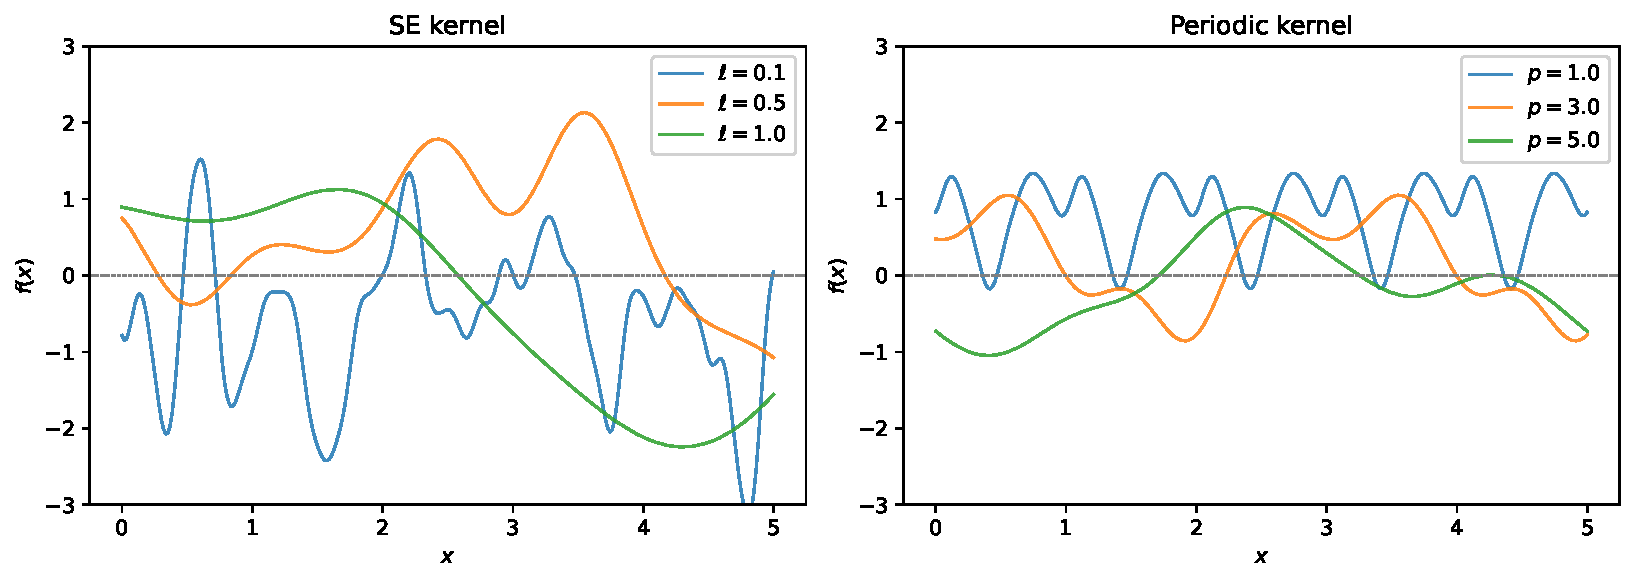
\includegraphics[keepaspectratio]{index_files/figure-pdf/fig-kernels-output-1.pdf}}

}

\caption{\label{fig-kernels}Prior samples from GPs with the SE kernel
(left) and the periodic kernel (right) under varying hyperparameters.}

\end{figure}%

The SE kernel, also called the radial basis function (RBF) kernel, is
defined as \begin{equation}\phantomsection\label{eq-se-kernel}{
k_{\text{SE}}(\mathbf{x}, \mathbf{x}') = \sigma_f^2 \exp\!\left(-\frac{\|\mathbf{x} - \mathbf{x}'\|^2}{2\ell^2}\right),
}\end{equation}

and is the most widely used GP kernel in practice
(\citeproc{ref-rasmussen_gaussian_2008}{Rasmussen and Williams 2008}). A
small \(\ell\) allows the function to vary rapidly over short distances,
producing rough wiggly samples, while a large \(\ell\) enforces smoothly
varying functions. The periodic kernel,
\begin{equation}\phantomsection\label{eq-periodic-kernel}{
k_{\text{per}}(\mathbf{x}, \mathbf{x}') = \sigma_f^2 \exp\!\left(-\frac{2\sin^2\!\left(\pi|\mathbf{x} - \mathbf{x}'|/p\right)}{\ell^2}\right),
}\end{equation}

explicitly encodes a repeating structure with period \(p\), making it
suitable for modelling seasonal or cyclical signals
(\citeproc{ref-rasmussen_gaussian_2008}{Rasmussen and Williams 2008}).
Kernels can also be combined --- sums and products of valid kernels are
themselves valid kernels --- enabling the construction of structured
priors that capture multiple scales or mixed behaviours
(\citeproc{ref-rasmussen_gaussian_2008}{Rasmussen and Williams 2008,
ch.\textasciitilde4}; \citeproc{ref-scholkopf_learning_2002}{Schölkopf
2002}).

\subsection{Choosing Kernel
Hyperparameters}\label{sec-kernel-hyperparams}

The kernel hyperparameters \(\boldsymbol{\theta}\) (e.g.~length-scale
\(\ell\), output scale \(\sigma_f^2\), noise variance \(\sigma_n^2\))
are not specified by the GP directly, and must be estimated from data.
The standard approach is to maximise the log marginal likelihood (LML)
of the observed data under the GP model, also known as \emph{type-II
maximum likelihood} or \emph{empirical Bayes}
(\citeproc{ref-mackay_practical_1992}{D. J. C. MacKay 1992};
\citeproc{ref-mackay_introduction_1998}{D. J. MacKay 1998};
\citeproc{ref-rasmussen_gaussian_2008}{Rasmussen and Williams 2008}),

\begin{equation}\phantomsection\label{eq-log-marginal-likelihood}{
\begin{aligned}
\log p(\mathbf{y} \mid \mathbf{X}, \boldsymbol{\theta}) &= -\frac{1}{2}\mathbf{y}^\top(K + \sigma_n^2\mathbf{I})^{-1}\mathbf{y} \quad\text{(data fit)} \\
&\quad - \frac{1}{2}\log |K + \sigma_n^2\mathbf{I}| \quad\text{(complexity penalty)} \\
&\quad - \frac{n}{2}\log 2\pi \quad\text{(normalisation constant)}.
\end{aligned}
}\end{equation}

This LML has 3 interpretable terms: the first encourages the model to
fit the data well, the second penalises overly complex models that can
fit many functions, and the third is a constant that ensures the
likelihood is properly normalised. The LML is typically maximised using
gradient-based optimisation (e.g.~L-BFGS or Adam
(\citeproc{ref-kingma_adam_2015}{Kingma and Ba 2015})), which is
tractable for exact GPs since the LML and its gradients can be computed
in \(\mathcal{O}(n^3)\) time via Cholesky decomposition of
\(K + \sigma_n^2\mathbf{I}\)
(\citeproc{ref-rasmussen_gaussian_2008}{Rasmussen and Williams 2008}).
However, the LML is non-convex and can have multiple local optima, so it
is common to perform multiple random restarts to increase the chances of
finding a good solution. Additionally, since kernel hyperparameters are
typically constrained to be positive, it is standard practice to
optimise them in log-space to ensure positivity and improve numerical
stability.

\subsection{GP Regression}\label{sec-gp-regression}

Given noisy training observations
\(\mathbf{y} = \mathbf{f} + \boldsymbol{\epsilon}\) with
\(\boldsymbol{\epsilon} \sim \mathcal{N}(\mathbf{0}, \sigma_n^2 \mathbf{I})\)
independent of \(\mathbf{f}\), the three blocks of the joint covariance
follow directly from the GP prior (see
Appendix~\ref{sec-covariance-blocks} for the full expansion):

\[
\begin{aligned}
\operatorname{Cov}[\mathbf{y}, \mathbf{y}] &= \operatorname{Cov}[\mathbf{f} + \boldsymbol{\epsilon}, \mathbf{f} + \boldsymbol{\epsilon}] = K + \sigma_n^2 \mathbf{I}, \\
\operatorname{Cov}[\mathbf{y}, f_*] &= \operatorname{Cov}[\mathbf{f} + \boldsymbol{\epsilon}, f(\mathbf{x}_*)] = \mathbf{k}_*, \\
\operatorname{Cov}[f_*, f_*] &= k(\mathbf{x}_*, \mathbf{x}_*) = k_{**},
\end{aligned}
\]

where \([\mathbf{k}_*]_i = k(\mathbf{x}_i, \mathbf{x}_*)\) and
\(k_{**} = k(\mathbf{x}_*, \mathbf{x}_*)\). Since \(\mathbf{y}\) and
\(f_*\) are jointly Gaussian as linear functions of the GP, the joint
distribution over training outputs and test value
\(f_* = f(\mathbf{x}_*)\) is:
\begin{equation}\phantomsection\label{eq-joint-gp}{
\begin{bmatrix} \mathbf{y} \\ f_* \end{bmatrix}
\sim
\mathcal{N}\!\left(
\mathbf{0},\;
\begin{bmatrix} K + \sigma_n^2 \mathbf{I} & \mathbf{k}_* \\ \mathbf{k}_*^\top & k_{**} \end{bmatrix}
\right).
}\end{equation} Conditioning on \(\mathbf{y}\) via the standard Gaussian
conditionals (\citeproc{ref-rasmussen_gaussian_2008}{Rasmussen and
Williams 2008}, Equation 2.19; \citeproc{ref-bishop_pattern_2006}{Bishop
2006, sec. 2.3}) gives the posterior predictive distribution:
\begin{equation}\phantomsection\label{eq-gp-predictive}{
p(f_* \mid \mathbf{x}_*, \mathbf{X}, \mathbf{y}) = \mathcal{N}\!\left(f_* \;\middle|\; \mathbf{k}_*^\top(K + \sigma_n^2\mathbf{I})^{-1}\mathbf{y},\; k_{**} - \mathbf{k}_*^\top(K+\sigma_n^2\mathbf{I})^{-1}\mathbf{k}_* + \sigma_n^2\right).
}\end{equation}

This is identical to the weight-space result in
Equation~\ref{eq-predictive-kernel-full}, but expressed in terms of the
kernel rather than the feature map. The posterior mean and covariance
are therefore the same as the predictive mean and variance from
Equation~\ref{eq-predictive-kernel}, and we can write the posterior GP
as:

\begin{equation}\phantomsection\label{eq-gp-posterior-moments}{
\begin{aligned}
m_{\text{post}}(\mathbf{x}_*) &= \mathbf{k}_*^\top(K + \sigma_n^2\mathbf{I})^{-1}\mathbf{y}, \\
k_{\text{post}}(\mathbf{x}_*, \mathbf{x}_*) &= k_{**} - \mathbf{k}_*^\top(K + \sigma_n^2\mathbf{I})^{-1}\mathbf{k}_*.
\end{aligned}
}\end{equation}

These expressions have intuitive interpretations: the posterior mean is
a linear combination of the observed outputs \(\mathbf{y}\), where the
weights are determined by the similarity between the test input and
training inputs as measured by the kernel. The posterior variance
\(k_{\text{post}}(\mathbf{x}_*, \mathbf{x}_*)\) is the prior variance at
\(\mathbf{x}_*\) minus a positive term that captures how much
information about \(f(\mathbf{x}_*)\) is contained in the training data
--- as more data are observed near \(\mathbf{x}_*\), this reduction
grows and uncertainty falls. Note that \(\sigma_n^2\) enters both
expressions through \((K + \sigma_n^2\mathbf{I})^{-1}\): noisier
observations are down-weighted, so the posterior retains more prior
uncertainty. The full predictive distribution over a new \emph{noisy}
observation \(y_* = f(\mathbf{x}_*) + \epsilon_*\) adds a further
\(+\sigma_n^2\) to the variance, as in Equation~\ref{eq-gp-predictive}.

Figure~\ref{fig-gp-regression} illustrates these properties : the left
panel shows three samples from the GP prior, and the right panel shows
the posterior after conditioning on observations, where uncertainty
collapses near the data and the posterior mean tracks the observations.

\begin{figure}[H]

\centering{

\pandocbounded{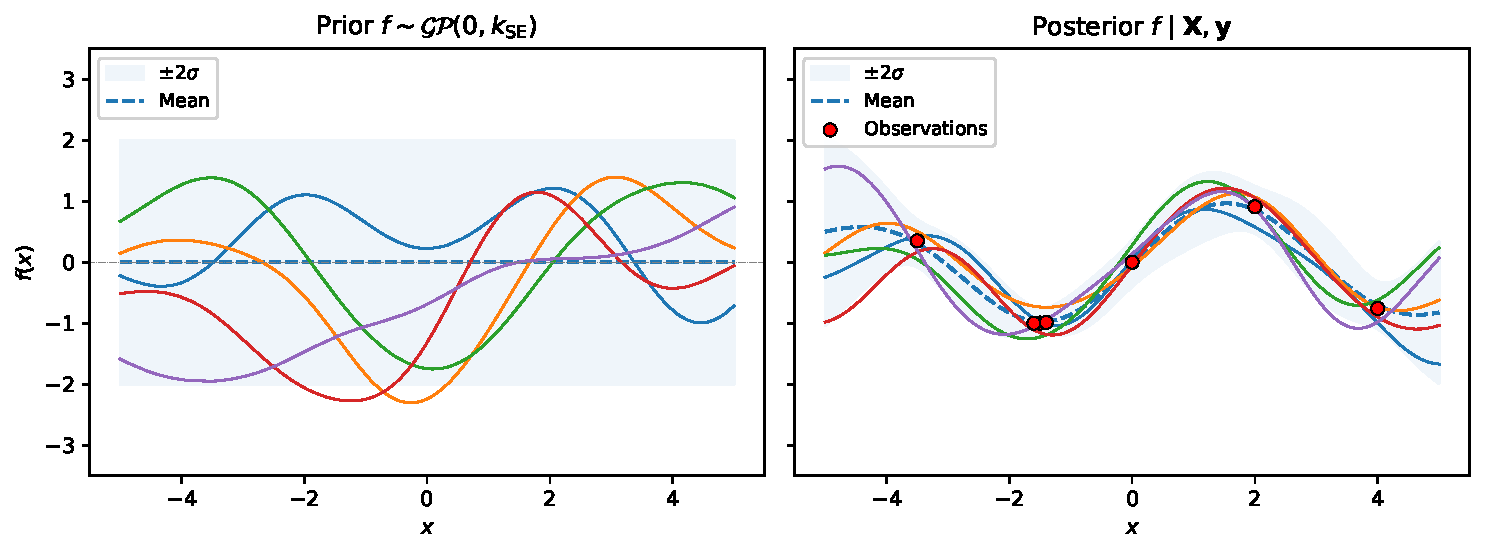
\includegraphics[keepaspectratio]{index_files/figure-pdf/fig-gp-regression-output-2.pdf}}

}

\caption{\label{fig-gp-regression}GP regression with an SE kernel. Left:
five prior samples before observing data. Right: posterior mean (blue),
95\% credible interval (shaded), and five posterior samples after
conditioning on five observations (red dots).}

\end{figure}%

\subsection{Training a GP}\label{sec-gp-training}

We showed in Section~\ref{sec-kernel-hyperparams} that the kernel
hyper-parameters \(\boldsymbol{\theta}\) can be estimated by maximising
the log marginal likelihood (LML) of the observed data. The LML is a
non-convex function of \(\boldsymbol{\theta}\), but its gradients can be
computed efficiently using matrix calculus and automatic
differentiation, enabling gradient-based optimisation methods such as
L-BFGS or Adam (\citeproc{ref-kingma_adam_2015}{Kingma and Ba 2015}) to
find good hyperparameter settings. However, computing the LML and its
gradients requires an \(\mathcal{O}(n^3)\) Cholesky decomposition of the
covariance matrix \(K + \sigma_n^2\mathbf{I}\), which is tractable for
moderate \(n\) but becomes prohibitive for large datasets, motivating
the development of sparse and approximate inference methods for scaling
GPs to larger problems (\citeproc{ref-snelson_sparse_2006}{Snelson and
Ghahramani 2006}; \citeproc{ref-titsias_variational_2009}{Titsias
2009}).

\subsubsection{Gradient of the Log Marginal
Likelihood}\label{gradient-of-the-log-marginal-likelihood}

We have the LML expression from
Equation~\ref{eq-log-marginal-likelihood}:
\[\log p(\mathbf{y} \mid \mathbf{X}, \boldsymbol{\theta}) = -\frac{1}{2}\mathbf{y}^\top(K + \sigma_n^2\mathbf{I})^{-1}\mathbf{y} - \frac{1}{2}\log |K + \sigma_n^2\mathbf{I}| - \frac{n}{2}\log 2\pi.\]

The gradient of the LML with respect to a hyperparameter \(\theta_j\)
can be derived using the matrix derivative trace formula
(\citeproc{ref-rasmussen_gaussian_2008}{Rasmussen and Williams 2008},
Equation 5.9), yielding:
\[  \frac{\partial \log p(\mathbf{y} \mid \mathbf{X}, \boldsymbol{\theta})}{\partial \theta_j} = \frac{1}{2}\mathbf{y}^\top(K + \sigma_n^2\mathbf{I})^{-1} \frac{\partial (K + \sigma_n^2\mathbf{I})}{\partial \theta_j} (K + \sigma_n^2\mathbf{I})^{-1} \mathbf{y} - \frac{1}{2}\text{tr}\!\left((K + \sigma_n^2\mathbf{I})^{-1} \frac{\partial (K + \sigma_n^2\mathbf{I})}{\partial \theta_j}\right). \]

This expression consists of two terms: the first encourages the model to
fit the data well by increasing the LML when the hyperparameter leads to
a better fit, while the second penalises overly complex models by
decreasing the LML when the hyperparameter increases model complexity.
These gradients can be computed efficiently using automatic
differentiation libraries, allowing for effective optimisation of the
hyperparameters.

In practice, the training loop iterates: (1) evaluate the negative LML
via Cholesky factorisation of \(K_\theta + \sigma_n^2\mathbf{I}\); (2)
backpropagate to obtain \(\partial \mathcal{L}/\partial \theta_j\) for
each hyperparameter; (3) apply an update step (e.g.~Adam). Because the
LML is non-convex, running multiple random restarts and keeping the
solution with the lowest negative LML is common practice.
Positive-constrained hyperparameters (\(\ell\), \(\sigma_f^2\),
\(\sigma_n^2\)) are parameterised in log-space throughout to ensure
positivity and improve the conditioning of the optimisation landscape.
Figure~\ref{fig-gp-training} illustrates the effect of training: a GP
with a poorly initialised length-scale produces an oversmoothed,
miscalibrated fit, while the same model after 50 Adam steps accurately
recovers the latent function.

\begin{figure}[H]

\centering{

\pandocbounded{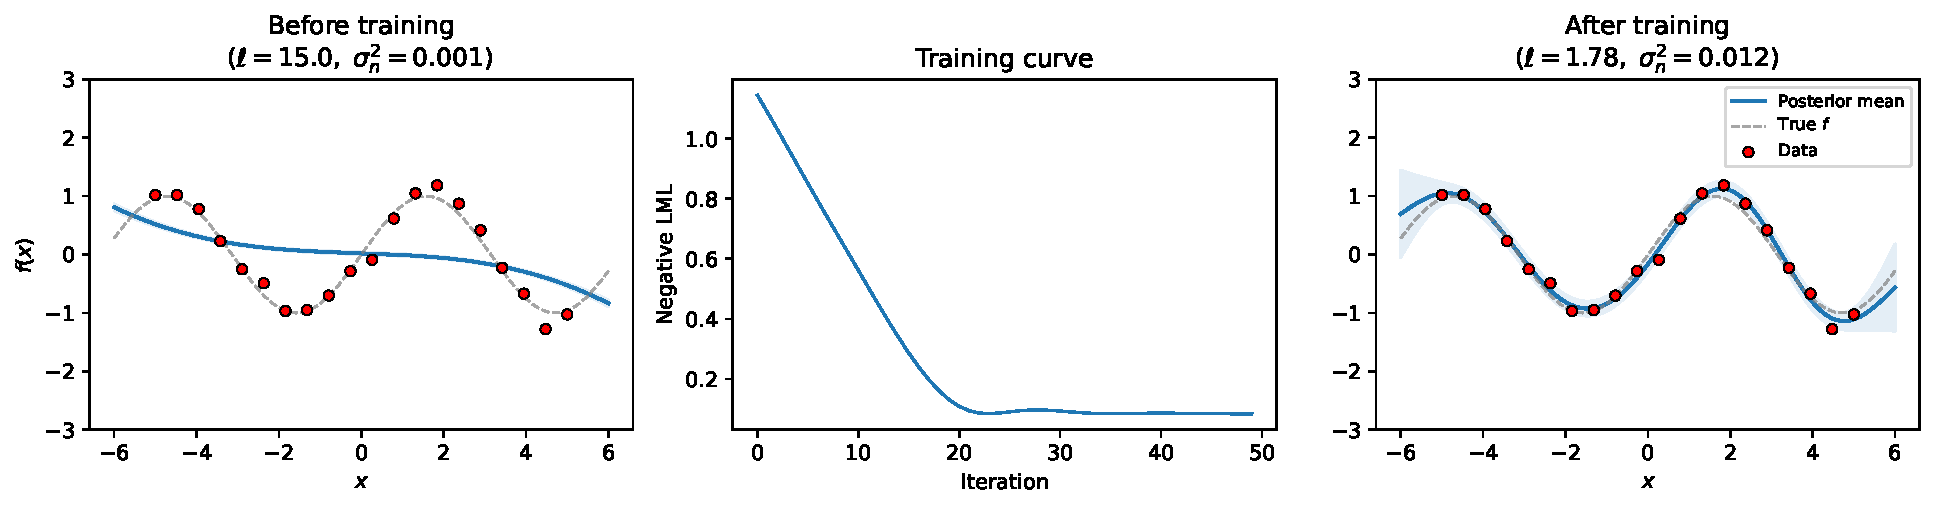
\includegraphics[keepaspectratio]{index_files/figure-pdf/fig-gp-training-output-2.pdf}}

}

\caption{\label{fig-gp-training}Effect of hyperparameter training on GP
fit. Left: GP with a deliberately large initial length-scale and
near-zero noise variance, producing a flat oversmoothed posterior.
Centre: negative log marginal likelihood during 50 Adam iterations.
Right: GP after training --- the learnt hyperparameter values are shown
in the subtitle.}

\end{figure}%

\subsection{Prediction}\label{sec-gp-prediction}

With hyperparameters fixed at their optimised values
\(\hat{\boldsymbol{\theta}}\), prediction reduces to evaluating the
posterior from Equation~\ref{eq-gp-posterior-moments} at any desired
test location \(\mathbf{x}_*\). The dominant cost is forming the
Cholesky factorisation
\(LL^\top = K_{\hat{\theta}} + \sigma_n^2\mathbf{I}\), which is
\(\mathcal{O}(n^3)\) and performed once. Once cached, evaluating the
predictive mean and variance at a new point requires only two triangular
solves and a kernel evaluation, costing \(\mathcal{O}(n)\) per point ---
making prediction cheap at test time once training has been completed.

The predictive variance at a test point \(\mathbf{x}_*\) decomposes
naturally into two contributions:
\begin{equation}\phantomsection\label{eq-variance-decomposition}{
\mathbb{V}[f_* \mid \mathbf{x}_*, \mathbf{X}, \mathbf{y}, \hat{\boldsymbol{\theta}}]
= \underbrace{k(\mathbf{x}_*, \mathbf{x}_*) - \mathbf{k}_*^\top(K + \sigma_n^2\mathbf{I})^{-1}\mathbf{k}_*}_{\text{epistemic (reducible)}}
+ \underbrace{\sigma_n^2}_{\text{aleatoric (irreducible)}},
}\end{equation}

where the first term is the \emph{epistemic} uncertainty --- reflecting
ignorance about the latent function \(f\) --- and the second is the
\emph{aleatoric} noise variance
(\citeproc{ref-kendall_what_2017}{Kendall and Gal 2017}). The epistemic
component shrinks as training observations accumulate near
\(\mathbf{x}_*\), and recovers the full prior variance
\(k(\mathbf{x}_*, \mathbf{x}_*)\) only in regions with no data. The
aleatoric term \(\sigma_n^2\) is present whenever a noisy observation
\(y_* = f(\mathbf{x}_*) + \epsilon_*\) is requested, but absent from the
latent predictive distribution over \(f(\mathbf{x}_*)\) itself. This
separation is a distinctive strength of the GP framework: the two
sources of uncertainty are quantified separately and automatically,
without requiring any post-hoc calibration
(\citeproc{ref-rasmussen_gaussian_2008}{Rasmussen and Williams 2008};
\citeproc{ref-kendall_what_2017}{Kendall and Gal 2017}).

This is visible in Figure~\ref{fig-gp-regression}: uncertainty collapses
near the training observations (low epistemic uncertainty) and inflates
in the gaps and at the extrapolation boundaries (high epistemic
uncertainty), while the posterior mean threads through the data.

\section{Deep Gaussian Processes}\label{sec-dgps}

The previous section established that GPs provide closed-form
predictions and uncertainty estimates, governed entirely by the choice
of kernel. However, the expressiveness of a single-layer GP is
fundamentally constrained by this kernel: a stationary kernel like the
squared exponential encodes a fixed notion of smoothness across the
entire input space, which may not match real-world data where patterns
vary in complexity across different regions.

Deep Gaussian Processes (DGPs) address this by composing multiple GP
layers hierarchically. Rather than relying on hand-crafted kernels, DGPs
learn representations at multiple levels of abstraction, much like deep
neural networks, while retaining Bayesian uncertainty quantification.
This section formalises the DGP model and shows why exact inference
becomes intractable in the deep setting, motivating the approximate
methods of Section~\ref{sec-learning}.

\subsection{Definition and Model
Formulation}\label{definition-and-model-formulation}

DGPs extend standard GPs by composing multiple GP layers in a
hierarchical structure (\citeproc{ref-damianou_deep_2013}{Damianou and
Lawrence 2013}). Instead of a single mapping from inputs to outputs,
DGPs construct a chain of latent function spaces, each transforming the
previous layer.

An \(L\)-layer DGP is defined by a sequence of latent functions
\(\{f^{(\ell)}\}_{\ell=1}^{L}\) where each function is drawn from a GP
prior conditioned on the output of the previous:

\begin{equation}\phantomsection\label{eq-dgp_definition}{
f^{(\ell)} \mid \mathbf{F}^{(\ell-1)} \sim \mathcal{GP}\left(0, k^{(\ell)}(\cdot, \cdot)\right), \quad \ell = 1, \ldots, L,
}\end{equation}

with the convention \(\mathbf{F}^{(0)} = \mathbf{X}\) (the observed
inputs). Each layer applies a freshly drawn GP function to the
\emph{outputs} of the previous layer --- the first layer warps the raw
inputs, the second warps those warped values, and so on. The model is a
learned chain of transformations, each inheriting all the uncertainty of
the layers before it.

For observed inputs \(\mathbf{X} \in \mathbb{R}^{n \times d_0}\) and
outputs \(\mathbf{y} \in \mathbb{R}^n\), the generative model proceeds
as:

\begin{equation}\phantomsection\label{eq-dgp_generative}{
\begin{aligned}
\mathbf{F}^{(1)} &= f^{(1)}(\mathbf{X}), & f^{(1)} &\sim \mathcal{GP}(0, k^{(1)}), \\
\mathbf{F}^{(2)} &= f^{(2)}(\mathbf{F}^{(1)}), & f^{(2)} &\sim \mathcal{GP}(0, k^{(2)}), \\
&\vdots \\
\mathbf{F}^{(L)} &= f^{(L)}(\mathbf{F}^{(L-1)}), & f^{(L)} &\sim \mathcal{GP}(0, k^{(L)}), \\
\mathbf{y} &= \mathbf{F}^{(L)} + \boldsymbol{\epsilon}, & \boldsymbol{\epsilon} &\sim \mathcal{N}(\mathbf{0}, \sigma_n^2 \mathbf{I}),
\end{aligned}
}\end{equation}

where \(\mathbf{F}^{(\ell)} \in \mathbb{R}^{n \times d_\ell}\) contains
function evaluations at layer \(\ell\) for all \(n\) data points, and
\(d_\ell\) is the output dimensionality of layer \(\ell\).

The covariance matrix at layer \(\ell\) is constructed from kernel
evaluations at the \emph{random} outputs of the previous layer:

\begin{equation}\phantomsection\label{eq-dgp_covariance_element}{
\left[K^{(\ell)}\right]_{ij} = k^{(\ell)}\left(\mathbf{f}_i^{(\ell-1)}, \mathbf{f}_j^{(\ell-1)}\right),
}\end{equation}

where \(\mathbf{f}_i^{(\ell-1)} \in \mathbb{R}^{d_{\ell-1}}\) is the
\(i\)-th row of \(\mathbf{F}^{(\ell-1)}\). When conditioned on the
outputs from layer \(\ell-1\), the distribution of
\(\mathbf{F}^{(\ell)}\) remains multivariate Gaussian:

\begin{equation}\phantomsection\label{eq-dgp_conditional_gaussian}{
p\left(\mathbf{F}^{(\ell)} \mid \mathbf{F}^{(\ell-1)}\right) = \mathcal{N}\left(\mathbf{F}^{(\ell)} \mid \mathbf{0}, K^{(\ell)}\right).
}\end{equation}

When \(\mathbf{F}^{(\ell-1)}\) is held fixed, this is identical to a
standard GP prior --- layer \(\ell\) behaves exactly like a regular GP
evaluated at those inputs. The difficulty arises only when
\(\mathbf{F}^{(\ell-1)}\) is random: the covariance matrix
\(K^{(\ell)}\) then becomes a random variable itself, and integrating
over it no longer yields a closed form.

The directed graph structure implies that each layer depends only on its
immediate predecessor (a Markov property), leading to a factorised joint
prior:

\begin{equation}\phantomsection\label{eq-dgp_joint_prior}{
p\left(\mathbf{F}^{(1)}, \ldots, \mathbf{F}^{(L)} \mid \mathbf{X}\right) = p\left(\mathbf{F}^{(1)} \mid \mathbf{X}\right) \prod_{\ell=2}^{L} p\left(\mathbf{F}^{(\ell)} \mid \mathbf{F}^{(\ell-1)}\right).
}\end{equation}

This follows from applying the chain rule and noting that
\(\mathbf{F}^{(\ell)} \perp \mathbf{F}^{(1:\ell-2)}, \mathbf{X} \mid \mathbf{F}^{(\ell-1)}\).
In plain terms: once you know what layer \(\ell\!-\!1\) output,
knowledge of all earlier layers gives no additional information about
layer \(\ell\). Practically, this means one can sample through the model
one layer at a time, discarding each layer's outputs once they have been
passed forward. The likelihood connects the final layer to observations
via
\(p(\mathbf{y} \mid \mathbf{F}^{(L)}) = \mathcal{N}(\mathbf{y} \mid \mathbf{F}^{(L)}, \sigma_n^2 \mathbf{I})\).

Equivalently, defining the composed function
\(f = f^{(L)} \circ f^{(L-1)} \circ \cdots \circ f^{(1)}\):

\begin{equation}\phantomsection\label{eq-dgp_composition}{
\mathbf{y} = f(\mathbf{X}) + \boldsymbol{\epsilon} = f^{(L)}(f^{(L-1)}(\cdots f^{(1)}(\mathbf{X}))) + \boldsymbol{\epsilon}.
}\end{equation}

When layers have output dimension \(d_\ell > 1\), the standard approach
uses independent GPs per output dimension:

\begin{equation}\phantomsection\label{eq-dgp_multi_output}{
\mathbf{F}^{(\ell)} = \left[\mathbf{f}^{(\ell,1)}, \ldots, \mathbf{f}^{(\ell,d_\ell)}\right], \quad f^{(\ell,j)} \stackrel{\text{ind}}{\sim} \mathcal{GP}\left(0, k^{(\ell)}\right).
}\end{equation}

This leads to \(\sum_{\ell=1}^{L} n \cdot d_\ell = O(nLd)\) total latent
variables.

Figure~\ref{fig-dgp-composition} illustrates the compositional structure
of a two-layer DGP. The first layer warps the input, and the second
layer operates on the warped space, producing a composed function that
would be difficult to represent with a single GP.

\begin{figure}[H]

\centering{

\pandocbounded{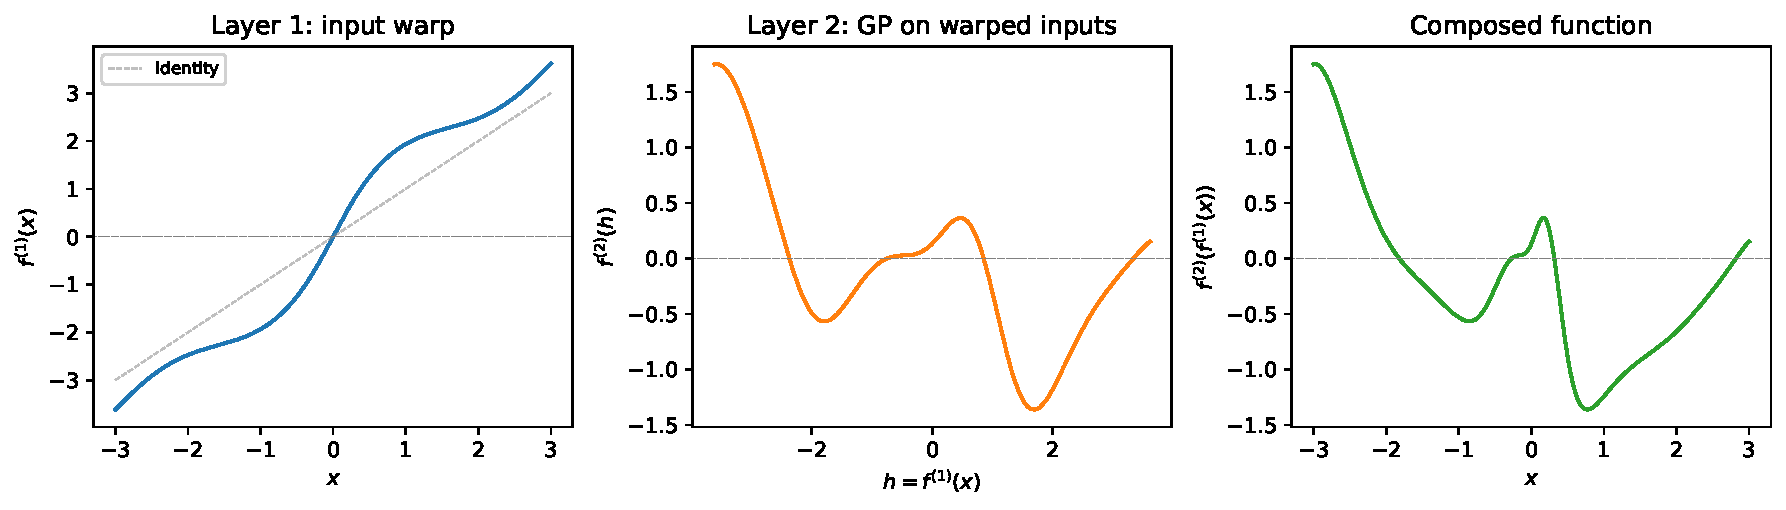
\includegraphics[keepaspectratio]{index_files/figure-pdf/fig-dgp-composition-output-1.pdf}}

}

\caption{\label{fig-dgp-composition}Compositional structure of a
two-layer DGP. Left: the first-layer function \(f^{(1)}\) warps the
input. Centre: the second-layer function \(f^{(2)}\) maps the warped
inputs to outputs. Right: the composed function
\(f^{(2)} \circ f^{(1)}\) exhibits non-stationary behaviour --- smooth
in some regions and rapidly varying in others --- that neither layer
alone could produce.}

\end{figure}%

The expressiveness of DGPs over standard GPs comes from this composition
(\citeproc{ref-damianou_deep_2013}{Damianou and Lawrence 2013};
\citeproc{ref-dunlop_how_2018}{Dunlop et al. 2018}). Even when each
layer uses a stationary kernel, the composed function yields a
non-stationary process. Consider the covariance of
\(g = f^{(2)} \circ f^{(1)}\):

\begin{equation}\phantomsection\label{eq-composed_covariance}{
\text{Cov}[g(\mathbf{x}), g(\mathbf{x}')] = \mathbb{E}_{f^{(1)}}\left[k^{(2)}\left(f^{(1)}(\mathbf{x}), f^{(1)}(\mathbf{x}')\right)\right].
}\end{equation}

This expectation depends on marginal distributions of
\(f^{(1)}(\mathbf{x})\) and \(f^{(1)}(\mathbf{x}')\), which change with
\(\mathbf{x}, \mathbf{x}'\) through \(k^{(1)}\). The composed covariance
is therefore not simply a function of \(\mathbf{x} - \mathbf{x}'\),
making the process non-stationary. This input-dependent structure lets
DGPs model functions with varying smoothness and lengthscale across
input space. To see why this is useful, imagine fitting a signal that is
smooth in some regions and rapidly varying in others: a single GP with a
fixed lengthscale must compromise, while a DGP can learn to ``stretch''
the input space in smooth regions and ``compress'' it in complex regions
through \(f^{(1)}\), giving the second layer an effectively adapted
coordinate system. {[}\textbf{TODO: CITE}{]}.

\subsection{Intractability of Exact
Inference}\label{intractability-of-exact-inference}

For standard single-layer GPs, the posterior
\(p(f_* \mid \mathbf{X}, \mathbf{y})\) and marginal likelihood
\(p(\mathbf{y} \mid \mathbf{X})\) give closed-form expressions due to
Gaussian conjugacy (\citeproc{ref-rasmussen_gaussian_2008}{Rasmussen and
Williams 2008}). In DGPs this is lost because composition of GPs
produces a non-Gaussian joint distribution.

The marginal likelihood requires integrating out all latent functions:

\begin{equation}\phantomsection\label{eq-dgp_marginal_likelihood}{
p(\mathbf{y} \mid \mathbf{X}) = \int p(\mathbf{y} \mid \mathbf{F}^{(L)}) \prod_{\ell=1}^{L} p(\mathbf{F}^{(\ell)} \mid \mathbf{F}^{(\ell-1)}) \, d\mathbf{F}^{(1)} \cdots d\mathbf{F}^{(L)},
}\end{equation}

where \(\mathbf{F}^{(0)} = \mathbf{X}\). This integral has no
closed-form solution for \(L \geq 2\) with non-degenerate kernels. The
fundamental obstacle is that the covariance matrix \(K^{(\ell)}\) at
each layer is a nonlinear function of \(\mathbf{F}^{(\ell-1)}\) --- the
very variables being integrated over --- so the integral cannot be
reorganised into the product-of-Gaussians form that makes single-layer
GP inference tractable.

To see why, consider a two-layer DGP. The covariance matrix \(K^{(2)}\)
depends on \(\mathbf{F}^{(1)}\) through
\([K^{(2)}]_{ij} = k^{(2)}(f_i^{(1)}, f_j^{(1)})\). For the squared
exponential kernel:

\begin{equation}\phantomsection\label{eq-se_random_inputs}{
k^{(2)}(h_1, h_2) = \sigma_f^2 \exp\left(-\frac{(h_1 - h_2)^2}{2\ell^2}\right),
}\end{equation}

this is a nonlinear function of the Gaussian random variables
\((f_i^{(1)}, f_j^{(1)})\). The integral

\[
\int \mathcal{N}(\mathbf{F}^{(2)} \mid \mathbf{0}, K^{(2)}(\mathbf{F}^{(1)})) \mathcal{N}(\mathbf{F}^{(1)} \mid \mathbf{0}, K^{(1)}) \, d\mathbf{F}^{(1)}
\]

is a mixture of Gaussians with continuously varying covariance.
Intuitively, for every possible realisation of \(\mathbf{F}^{(1)}\)
there is a different Gaussian over \(\mathbf{F}^{(2)}\); marginalising
out \(\mathbf{F}^{(1)}\) means averaging together infinitely many
Gaussians with different shapes, producing a result that is
heavier-tailed and more complex than any individual Gaussian component.
No closed form exists for these integrals.

As well as the intractability of the marginal likelihood, the resulting
distribution over outputs is non-Gaussian. Consider a two-layer DGP with
first-layer outputs \(h_1 = f^{(1)}(x_1)\), \(h_2 = f^{(1)}(x_2)\). From
the GP prior:

\begin{equation}\phantomsection\label{eq-first_layer_joint}{
\begin{bmatrix} h_1 \\ h_2 \end{bmatrix} \sim \mathcal{N}\left(\mathbf{0}, \begin{bmatrix} k^{(1)}_{11} & k^{(1)}_{12} \\ k^{(1)}_{12} & k^{(1)}_{22} \end{bmatrix}\right).
}\end{equation}

Conditioned on \((h_1, h_2)\), the outputs follow:

\begin{equation}\phantomsection\label{eq-second_layer_conditional}{
\begin{bmatrix} y_1 \\ y_2 \end{bmatrix} \Bigg| h_1, h_2 \sim \mathcal{N}\left(\mathbf{0}, \begin{bmatrix} k^{(2)}(h_1, h_1) & k^{(2)}(h_1, h_2) \\ k^{(2)}(h_1, h_2) & k^{(2)}(h_2, h_2) \end{bmatrix}\right).
}\end{equation}

The marginal distribution

\begin{equation}\phantomsection\label{eq-marginal_y}{
p(y_1, y_2) = \int p(y_1, y_2 \mid h_1, h_2) \, p(h_1, h_2) \, dh_1 \, dh_2
}\end{equation}

is a continuous mixture of Gaussians with varying covariance matrices.
Since \(k^{(2)}(h_1, h_2)\) is a nonlinear function of \((h_1, h_2)\),
this mixture is not Gaussian.

This can be verified by noting that a Gaussian mixture with continuously
varying covariance matrices produces a distribution whose higher moments
(e.g., kurtosis) differ from those of any single Gaussian. In
particular, the marginal density of \(y_1\) under such a mixture is
generally heavier-tailed than any individual Gaussian component
(\citeproc{ref-gelman_bayesian_2025}{Gelman et al. 2025}).

The posterior over all latent functions is:

\begin{equation}\phantomsection\label{eq-dgp_posterior}{
p(\mathbf{F}^{(1:L)} \mid \mathbf{X}, \mathbf{y}) = \frac{p(\mathbf{y} \mid \mathbf{F}^{(L)}) \prod_{\ell=1}^{L} p(\mathbf{F}^{(\ell)} \mid \mathbf{F}^{(\ell-1)})}{p(\mathbf{y} \mid \mathbf{X})}.
}\end{equation}

Since both the numerator (a product of coupled Gaussians) and the
denominator (the intractable marginal likelihood) lack closed forms,
exact posterior computation is infeasible.

Even numerical integration is impractical. The integration is over
\(\sum_{\ell=1}^{L} n d_\ell\) continuous variables, which cannot be
factored across layers due to kernel dependencies. This motivates the
development of approximate inference methods for DGP learning
(\citeproc{ref-damianou_deep_2013}{Damianou and Lawrence 2013};
\citeproc{ref-salimbeni_doubly_2017}{Salimbeni and Deisenroth 2017}).

\section{Learning in GP and DGP Models}\label{sec-learning}

The previous section showed that DGPs offer richer modelling capacity
than standard GPs, but at the cost of tractable inference. This section
develops the framework for learning in both settings.

We briefly revisit hyperparameter learning in standard GPs --- focusing
on how the marginal likelihood arises by integrating out function values
--- to identify the structural property that is lost in DGPs. We then
introduce variational inference for approximating intractable
posteriors, build to sparse variational methods that reduce computation
from \(O(n^3)\) to \(O(nm^2)\), and finally extend these ideas to DGPs
through doubly stochastic variational inference.

\subsection{Learning in Standard GPs}\label{learning-in-standard-gps}

As established in Section~\ref{sec-kernel-hyperparams}, GP
hyperparameters \(\boldsymbol{\theta}\) are learned by maximising the
log marginal likelihood (LML). It is worth seeing explicitly how this
LML arises by integrating out the latent function values \(\mathbf{f}\),
since this tractability is precisely what is lost in DGPs.

Starting from the GP prior
\(\mathbf{f} \mid \mathbf{X} \sim \mathcal{N}(\mathbf{0}, K_{\boldsymbol{\theta}})\)
and likelihood
\(\mathbf{y} \mid \mathbf{f} \sim \mathcal{N}(\mathbf{f}, \sigma_n^2 \mathbf{I})\),
Gaussian--Gaussian conjugacy
(\citeproc{ref-bernardo_bayesian_2000}{Bernardo and Smith 2000}) allows
the integral over function values to be computed in closed form:
\begin{equation}\phantomsection\label{eq-gp_marginal_likelihood}{
p(\mathbf{y} \mid \mathbf{X}, \boldsymbol{\theta}) = \int p(\mathbf{y} \mid \mathbf{f}) p(\mathbf{f} \mid \mathbf{X}, \boldsymbol{\theta}) \, d\mathbf{f} = \mathcal{N}(\mathbf{y} \mid \mathbf{0}, K_{\boldsymbol{\theta}} + \sigma_n^2 \mathbf{I}),
}\end{equation} giving the LML of
Equation~\ref{eq-log-marginal-likelihood}. The key step is that a
Gaussian prior on \(\mathbf{f}\) multiplied by a Gaussian likelihood in
\(\mathbf{y}\) integrates analytically: the product of two Gaussians is
proportional to a Gaussian, so the \(\mathbf{f}\)-integral collapses to
a single multivariate normal with covariance
\(K_{\boldsymbol{\theta}} + \sigma_n^2 \mathbf{I}\). This closed-form
collapse is precisely what is lost in DGPs, where the covariance depends
on random latent variables. Hyperparameters are found via gradient
ascent; the gradient with respect to \(\theta_j\) is
(\citeproc{ref-rasmussen_gaussian_2008}{Rasmussen and Williams 2008}):

\begin{equation}\phantomsection\label{eq-gradient}{
\frac{\partial \log p(\mathbf{y})}{\partial \theta_j} = \frac{1}{2}\operatorname{tr}\left((\boldsymbol{\alpha} \boldsymbol{\alpha}^\top - K_y^{-1}) \frac{\partial K_y}{\partial \theta_j}\right),
}\end{equation}

where \(\boldsymbol{\alpha} = K_y^{-1} \mathbf{y}\) and
\(K_y = K_{\boldsymbol{\theta}} + \sigma_n^2 \mathbf{I}\). The matrix
\(\boldsymbol{\alpha} \boldsymbol{\alpha}^\top - K_y^{-1}\) has a
natural interpretation: \(\boldsymbol{\alpha} \boldsymbol{\alpha}^\top\)
is a rank-one outer product that captures how the data predicts itself
under the current model, while \(K_y^{-1}\) reflects the full model
uncertainty; a large positive difference for
\(\partial K_y / \partial \theta_j\) indicates that increasing
\(\theta_j\) improves the data fit more than it increases model
complexity. This follows from the matrix calculus identities
\(\frac{\partial}{\partial \theta} \log|K| = \operatorname{tr}(K^{-1} \frac{\partial K}{\partial \theta})\)
and
\(\frac{\partial K^{-1}}{\partial \theta} = -K^{-1} \frac{\partial K}{\partial \theta} K^{-1}\).

Each gradient step requires \(K_y^{-1}\), computed via Cholesky
decomposition at \(O(n^3)\) cost with \(O(n^2)\) storage
(\citeproc{ref-rasmussen_gaussian_2008}{Rasmussen and Williams 2008}).
For small to moderate datasets (\(n \lesssim 10{,}000\)) this is
typically feasible and remains the gold standard: the LML gradients are
exact, and no approximation is introduced beyond the choice of kernel.
For larger datasets the cubic cost becomes prohibitive, motivating the
sparse variational approach of the following section.

\subsection{Variational Inference}\label{variational-inference}

When exact inference is intractable, variational inference provides a
principled approximation framework
(\citeproc{ref-jordan_introduction_1999}{Jordan et al. 1999};
\citeproc{ref-blei_variational_2017}{Blei, Kucukelbir, and McAuliffe
2017}). The idea is to approximate the true posterior
\(p(\mathbf{z} \mid \mathbf{y})\) with a tractable distribution
\(q(\mathbf{z})\), chosen to minimise the Kullback--Leibler divergence
between them.

For latent variables \(\mathbf{z}\) and observations \(\mathbf{y}\), the
log marginal likelihood separates as:

\begin{equation}\phantomsection\label{eq-vi_decomposition}{
\log p(\mathbf{y}) = \mathcal{L}(q) + \operatorname{KL}(q(\mathbf{z}) \| p(\mathbf{z} \mid \mathbf{y})),
}\end{equation}

where the evidence lower bound (ELBO) is:

\begin{equation}\phantomsection\label{eq-elbo}{
\mathcal{L}(q) = \mathbb{E}_{q(\mathbf{z})}[\log p(\mathbf{y}, \mathbf{z})] - \mathbb{E}_{q(\mathbf{z})}[\log q(\mathbf{z})] = \mathbb{E}_{q(\mathbf{z})}[\log p(\mathbf{y} \mid \mathbf{z})] - \operatorname{KL}(q(\mathbf{z}) \| p(\mathbf{z})).
}\end{equation}

Since KL divergence is non-negative,
\(\mathcal{L}(q) \leq \log p(\mathbf{y})\) with equality when
\(q(\mathbf{z}) = p(\mathbf{z} \mid \mathbf{y})\). This is the central
insight: rather than computing the intractable posterior directly, we
turn the problem into an optimisation --- find the \(q\) that maximises
the ELBO, which simultaneously tightens the bound and minimises the
error of our approximation.

To show Equation~\ref{eq-vi_decomposition}, start from the definition of
KL divergence:

\[
\begin{aligned}
\operatorname{KL}(q \| p) &= \mathbb{E}_{q(\mathbf{z})}\left[\log \frac{q(\mathbf{z})}{p(\mathbf{z} \mid \mathbf{y})}\right] = \mathbb{E}_{q(\mathbf{z})}[\log q(\mathbf{z})] - \mathbb{E}_{q(\mathbf{z})}[\log p(\mathbf{z} \mid \mathbf{y})] \\
&= \mathbb{E}_{q(\mathbf{z})}[\log q(\mathbf{z})] - \mathbb{E}_{q(\mathbf{z})}[\log p(\mathbf{y}, \mathbf{z})] + \log p(\mathbf{y}).
\end{aligned}
\]

Rearranging gives Equation~\ref{eq-vi_decomposition}. Since
\(\operatorname{KL}(q \| p)\) cannot be computed directly (it is
intractable), we instead maximise the ELBO, which is equivalent to
minimising KL divergence. This replaces an intractable posterior
computation with a tractable optimisation problem --- the core trade of
variational inference.

The second form Equation~\ref{eq-elbo} illuminates the ELBO's structure.
The expected log-likelihood
\(\mathbb{E}_{q}[\log p(\mathbf{y} \mid \mathbf{z})]\) encourages \(q\)
to concentrate where the data is well-explained, while the KL term
\(\operatorname{KL}(q \| p(\mathbf{z}))\) regularises \(q\) toward the
prior, preventing overfitting (\citeproc{ref-bishop_pattern_2006}{Bishop
2006}). This trade-off mirrors the data-fit versus complexity balance in
exact Bayesian inference.

For the models in this dissertation, variational inference serves two
purposes: enabling scalability to large datasets, and handling the
hierarchical structure of DGPs where function values at each layer
cannot be analytically integrated out. The latent variables
\(\mathbf{z}\) correspond to function values \(\mathbf{f}\), and the
variational distribution is usually chosen to be Gaussian:

\begin{equation}\phantomsection\label{eq-variational_gaussian}{
q(\mathbf{f}) = \mathcal{N}(\mathbf{f} \mid \mathbf{m}, S),
}\end{equation}

with variational parameters \(\mathbf{m} \in \mathbb{R}^n\) and
\(S \in \mathbb{R}^{n \times n}\) (positive definite). This balances
expressiveness with computational tractability. The expectations under
\(q\) can often be computed analytically for standard likelihood
functions.

With this Gaussian choice, the KL term has closed form:

\begin{equation}\phantomsection\label{eq-kl_gaussian}{
\operatorname{KL}(q(\mathbf{f}) \| p(\mathbf{f})) = \frac{1}{2}\left[\operatorname{tr}(K^{-1}S) + \mathbf{m}^\top K^{-1} \mathbf{m} - n + \log|K| - \log|S|\right],
}\end{equation}

where \(K\) is the prior covariance. Each term has a clear role:
\(\mathbf{m}^\top K^{-1} \mathbf{m}\) penalises the variational mean for
straying far from zero in units of the prior length-scale;
\(\operatorname{tr}(K^{-1}S)\) penalises the variational covariance for
being larger than the prior; and \(\log|K| - \log|S|\) is a log-volume
ratio that rewards \(q\) for being more concentrated than the prior.
Together they ensure \(q\) cannot deviate from \(p(\mathbf{f})\) without
paying a KL cost. Optimisation over a full-rank matrix
\(S \in \mathbb{R}^{n \times n}\) still involves \(O(n^2)\) parameters,
which becomes problematic for large \(n\). The key to resolving this is
to restrict the variational family to a lower-dimensional subspace
defined by \(m \ll n\) \emph{inducing points}, as developed in the
following section.

\subsection{Sparse Variational GPs}\label{sparse-variational-gps}

The \(O(n^3)\) cost of standard GP inference becomes prohibitive for
large datasets. Sparse methods address this by using \(m \ll n\)
\emph{inducing points} that summarise the data, reducing complexity to
\(O(nm^2)\)
(\citeproc{ref-quinonero-candela_unifying_2005}{Quinonero-Candela and
Rasmussen 2005}; \citeproc{ref-titsias_variational_2009}{Titsias 2009}).

Consider inducing inputs \(\mathbf{Z} = \{\mathbf{z}_j\}_{j=1}^m\) with
function values \(\mathbf{u} = f(\mathbf{Z}) \in \mathbb{R}^m\). From
the prior, the joint distribution of function values \(\mathbf{f}\) at
training inputs and inducing values \(\mathbf{u}\) is:

\begin{equation}\phantomsection\label{eq-joint_f_u}{
\begin{bmatrix} \mathbf{f} \\ \mathbf{u} \end{bmatrix} \sim \mathcal{N}\left(\mathbf{0}, \begin{bmatrix} K_{ff} & K_{fu} \\ K_{uf} & K_{uu} \end{bmatrix}\right),
}\end{equation}

where \(K_{ff} = K(\mathbf{X}, \mathbf{X})\),
\(K_{fu} = K(\mathbf{X}, \mathbf{Z})\), and
\(K_{uu} = K(\mathbf{Z}, \mathbf{Z})\). The cross-covariance \(K_{fu}\)
encodes how strongly each training point correlates with each inducing
point: if inducing points are placed where the data concentrates,
\(K_{fu}\) will be large and the \(m\) inducing values will carry most
of the information about the \(n\) function values.

Titsias (\citeproc{ref-titsias_variational_2009}{2009}) introduced a
variational framework that treats \(\mathbf{Z}\) as variational
parameters rather than fixed pseudo-inputs. The key idea is to use the
conditional \(p(\mathbf{f} \mid \mathbf{u})\) from the prior and place a
variational distribution on \(\mathbf{u}\):

\begin{equation}\phantomsection\label{eq-sparse_variational_form}{
q(\mathbf{f}, \mathbf{u}) = p(\mathbf{f} \mid \mathbf{u}) q(\mathbf{u}),
}\end{equation}

where \(q(\mathbf{u}) = \mathcal{N}(\mathbf{u} \mid \mathbf{m}, S)\)
with variational parameters \(\mathbf{m} \in \mathbb{R}^m\) and
\(S \in \mathbb{R}^{m \times m}\). Rather than placing a variational
distribution directly on all \(n\) function values \(\mathbf{f}\), we
only learn a distribution over the \(m\) inducing values \(\mathbf{u}\)
and use the GP conditional \(p(\mathbf{f} \mid \mathbf{u})\) to fill in
the rest. This reduces the variational parameter count from \(O(n^2)\)
to \(O(m^2)\).

\begin{equation}\phantomsection\label{eq-conditional_f_given_u}{
p(\mathbf{f} \mid \mathbf{u}) = \mathcal{N}(\mathbf{f} \mid K_{fu} K_{uu}^{-1} \mathbf{u}, \, K_{ff} - K_{fu} K_{uu}^{-1} K_{uf}).
}\end{equation}

This is the standard GP predictive formula: the conditional mean
\(K_{fu}K_{uu}^{-1}\mathbf{u}\) is a weighted combination of inducing
values, with weights proportional to how correlated each training point
is with each inducing point. The conditional variance
\(K_{ff} - K_{fu}K_{uu}^{-1}K_{uf}\) is the prior variance reduced by
the information the inducing points provide --- it vanishes at the
inducing locations themselves.

Marginalising out \(\mathbf{u}\), the variational distribution over
\(\mathbf{f}\) is:

\begin{equation}\phantomsection\label{eq-marginal_q_f}{
q(\mathbf{f}) = \int p(\mathbf{f} \mid \mathbf{u}) q(\mathbf{u}) \, d\mathbf{u} = \mathcal{N}(\mathbf{f} \mid K_{fu} K_{uu}^{-1} \mathbf{m}, \, K_{ff} - K_{fu} K_{uu}^{-1} K_{uf} + K_{fu} K_{uu}^{-1} S K_{uu}^{-1} K_{uf}).
}\end{equation}

Compared to the conditional
\(p(\mathbf{f} \mid \mathbf{u} = \mathbf{m})\), the variational
posterior \(q(\mathbf{f})\) adds the term
\(K_{fu}K_{uu}^{-1}SK_{uu}^{-1}K_{uf}\) to the variance; this restores
the uncertainty lost by treating \(\mathbf{u}\) as fixed at
\(\mathbf{m}\), so \(q(\mathbf{f})\) correctly reflects that our beliefs
about \(\mathbf{u}\) are not perfectly sharp.

The ELBO for this sparse model is
(\citeproc{ref-titsias_variational_2009}{Titsias 2009}):

\begin{equation}\phantomsection\label{eq-sparse_elbo}{
\mathcal{L} = \mathbb{E}_{q(\mathbf{f})}[\log p(\mathbf{y} \mid \mathbf{f})] - \operatorname{KL}(q(\mathbf{u}) \| p(\mathbf{u})).
}\end{equation}

The KL term has closed form:

\begin{equation}\phantomsection\label{eq-kl_inducing}{
\operatorname{KL}(q(\mathbf{u}) \| p(\mathbf{u})) = \frac{1}{2}\left[\operatorname{tr}(K_{uu}^{-1}S) + \mathbf{m}^\top K_{uu}^{-1} \mathbf{m} - m + \log|K_{uu}| - \log|S|\right].
}\end{equation}

For Gaussian likelihoods
\(p(\mathbf{y} \mid \mathbf{f}) = \mathcal{N}(\mathbf{y} \mid \mathbf{f}, \sigma_n^2 \mathbf{I})\),
the expected log-likelihood can be computed in closed form, yielding a
fully analytical ELBO. Optimal parameters satisfy:

\begin{equation}\phantomsection\label{eq-optimal_params}{
\begin{aligned}
S^{-1} &= K_{uu}^{-1} + \sigma_n^{-2} K_{uu}^{-1} K_{uf} K_{fu} K_{uu}^{-1}, \\
\mathbf{m} &= \sigma_n^{-2} S K_{uu}^{-1} K_{uf} \mathbf{y}.
\end{aligned}
}\end{equation}

With inducing points, predictions at test inputs \(\mathbf{X}_*\)
follow:

\begin{equation}\phantomsection\label{eq-sparse_predictions}{
\begin{aligned}
\mathbb{E}[f_*] &= K_{*u} K_{uu}^{-1} \mathbf{m}, \\
\text{Var}[f_*] &= K_{**} - K_{*u} K_{uu}^{-1} (K_{uu} - S) K_{uu}^{-1} K_{u*}.
\end{aligned}
}\end{equation}

The computational scaling is \(O(m^3)\) for inverting \(K_{uu}\),
\(O(nm^2)\) for matrix products involving \(K_{fu}\), and \(O(m^2)\)
storage for variational parameters. Inducing locations \(\mathbf{Z}\)
can be jointly optimised with hyperparameters \(\boldsymbol{\theta}\)
and variational parameters \((\mathbf{m}, S)\) by gradient ascent on the
ELBO.

\subsubsection{Stochastic Optimisation via
Minibatches}\label{stochastic-optimisation-via-minibatches}

Even at \(O(nm^2)\) per gradient step, iterating over the full dataset
each step becomes expensive for large \(n\). For Gaussian likelihoods
the expected log-likelihood in Equation~\ref{eq-sparse_elbo} decomposes
over individual data points:
\begin{equation}\phantomsection\label{eq-ell_decomposition}{
\mathbb{E}_{q(\mathbf{f})}[\log p(\mathbf{y} \mid \mathbf{f})] = \sum_{i=1}^n \mathbb{E}_{q(f_i)}[\log p(y_i \mid f_i)],
}\end{equation} since
\(p(\mathbf{y} \mid \mathbf{f}) = \prod_i p(y_i \mid f_i)\) and the
marginals
\(q(f_i) = \mathcal{N}(f_i \mid [K_{fu}K_{uu}^{-1}\mathbf{m}]_i,\, [K_{ff} - K_{fu}K_{uu}^{-1}(K_{uu}-S)K_{uu}^{-1}K_{uf}]_{ii})\)
are available in closed form. The KL term does not depend on the data
and can be evaluated once per step. This per-point structure means the
ELBO can be estimated unbiasedly from a random minibatch
\(\mathcal{B} \subset \{1,\ldots,n\}\)
(\citeproc{ref-hensman_gaussian_2013}{Hensman, Fusi, and Lawrence
2013}): \begin{equation}\phantomsection\label{eq-sparse_minibatch_elbo}{
\hat{\mathcal{L}} = \frac{n}{|\mathcal{B}|} \sum_{i \in \mathcal{B}} \mathbb{E}_{q(f_i)}[\log p(y_i \mid f_i)] - \operatorname{KL}(q(\mathbf{u}) \| p(\mathbf{u})).
}\end{equation} The factor \(n/|\mathcal{B}|\) re-scales the minibatch
sum so that it is an unbiased estimate of the full sum over all \(n\)
points: a minibatch of 100 data points still gives a correctly-scaled
estimate for a dataset of 100,000. Each step now costs
\(O(|\mathcal{B}|m^2 + m^3)\), making gradient-based optimisation
tractable even for very large datasets. This minibatch decomposition
carries directly into the doubly stochastic DGP estimator
Equation~\ref{eq-dsvi_mc_elbo}, which applies the same per-point
factorisation across all layers.

This sparse variational framework forms the foundation for scalable DGP
inference, with each layer maintaining its own set of inducing points.

\subsection{Variational Inference for
DGPs}\label{variational-inference-for-dgps}

Given the intractability of computing the exact posterior in DGPs,
variational inference provides the primary framework for DGP learning
(\citeproc{ref-damianou_deep_2013}{Damianou and Lawrence 2013}). The
approach extends the sparse variational GP framework by introducing
inducing points at each layer.

For an \(L\)-layer DGP, let
\(\mathbf{Z}^{(\ell)} \in \mathbb{R}^{m_\ell \times d_{\ell-1}}\) denote
inducing inputs at layer \(\ell\), with corresponding inducing outputs
\(\mathbf{U}^{(\ell)} = f^{(\ell)}(\mathbf{Z}^{(\ell)}) \in \mathbb{R}^{m_\ell \times d_\ell}\).
Following Damianou and Lawrence
(\citeproc{ref-damianou_deep_2013}{2013}), the variational distribution
factorises across layers:

\begin{equation}\phantomsection\label{eq-dgp_variational_factorization}{
q(\{\mathbf{F}^{(\ell)}, \mathbf{U}^{(\ell)}\}_{\ell=1}^L) = \prod_{\ell=1}^{L} p(\mathbf{F}^{(\ell)} \mid \mathbf{U}^{(\ell)}, \mathbf{F}^{(\ell-1)}) q(\mathbf{U}^{(\ell)}),
}\end{equation}

where
\(q(\mathbf{U}^{(\ell)}) = \mathcal{N}(\mathbf{U}^{(\ell)} \mid \mathbf{M}^{(\ell)}, \mathbf{S}^{(\ell)})\)
with variational parameters
\(\mathbf{M}^{(\ell)} \in \mathbb{R}^{m_\ell \times d_\ell}\) and
covariances \(\mathbf{S}^{(\ell)}\). The factorisation is a key design
choice: rather than placing a variational distribution over each layer's
full \(n \times d_\ell\) output matrix, we only learn distributions over
the much smaller \(m_\ell \times d_\ell\) inducing outputs at each
layer; the per-layer GP conditional
\(p(\mathbf{F}^{(\ell)} \mid \mathbf{U}^{(\ell)}, \mathbf{F}^{(\ell-1)})\)
then propagates information from inducing values to all training points.

The conditional
\(p(\mathbf{F}^{(\ell)} \mid \mathbf{U}^{(\ell)}, \mathbf{F}^{(\ell-1)})\)
uses the GP prior structure. For layer \(\ell\) with inputs from the
previous layer \(\mathbf{F}^{(\ell-1)}\) and inducing inputs
\(\mathbf{Z}^{(\ell)}\):

\begin{equation}\phantomsection\label{eq-dgp_layer_conditional}{
p(\mathbf{F}^{(\ell)} \mid \mathbf{U}^{(\ell)}, \mathbf{F}^{(\ell-1)}) = \mathcal{N}\left(\mathbf{F}^{(\ell)} \mid A^{(\ell)} \mathbf{U}^{(\ell)}, \, K^{(\ell)}_{ff} - A^{(\ell)} K^{(\ell)}_{uu} A^{(\ell)\top}\right),
}\end{equation}

where \(A^{(\ell)} = K^{(\ell)}_{fu} (K^{(\ell)}_{uu})^{-1}\).
Crucially, the covariance matrices \(K^{(\ell)}_{ff}\),
\(K^{(\ell)}_{fu}\), and \(K^{(\ell)}_{uu}\) depend on the random inputs
\(\mathbf{F}^{(\ell-1)}\), creating dependencies across layers.

The ELBO for DGPs is:

\begin{equation}\phantomsection\label{eq-dgp_elbo}{
\mathcal{L} = \mathbb{E}_{q(\mathbf{F}^{(1:L)})}[\log p(\mathbf{y} \mid \mathbf{F}^{(L)})] - \sum_{\ell=1}^{L} \operatorname{KL}(q(\mathbf{U}^{(\ell)}) \| p(\mathbf{U}^{(\ell)})).
}\end{equation}

The structure is intuitive: there is one data-fit term (the expected
log-likelihood at the final layer) and one KL ``regulariser'' per layer,
penalising each layer's variational posterior for deviating from its GP
prior. The KL terms have closed form since both
\(q(\mathbf{U}^{(\ell)})\) and \(p(\mathbf{U}^{(\ell)})\) are Gaussian.
However, the expected log-likelihood requires integration over all layer
outputs \(\mathbf{F}^{(1:L)}\), which is intractable due to the nested
structure.

The expectation in Equation~\ref{eq-dgp_elbo} involves:

\begin{equation}\phantomsection\label{eq-dgp_nested_expectation}{
\mathbb{E}_{q}[\log p(\mathbf{y} \mid \mathbf{F}^{(L)})] = \int \cdots \int \log p(\mathbf{y} \mid \mathbf{F}^{(L)}) \prod_{\ell=1}^{L} q(\mathbf{F}^{(\ell)} \mid \mathbf{F}^{(\ell-1)}) \, d\mathbf{F}^{(1)} \cdots d\mathbf{F}^{(L)},
}\end{equation}

where \(q(\mathbf{F}^{(\ell)} \mid \mathbf{F}^{(\ell-1)})\) is obtained
by integrating out \(\mathbf{U}^{(\ell)}\):

\begin{equation}\phantomsection\label{eq-marginal_q_layer}{
q(\mathbf{F}^{(\ell)} \mid \mathbf{F}^{(\ell-1)}) = \int p(\mathbf{F}^{(\ell)} \mid \mathbf{U}^{(\ell)}, \mathbf{F}^{(\ell-1)}) q(\mathbf{U}^{(\ell)}) \, d\mathbf{U}^{(\ell)}.
}\end{equation}

This integral is Gaussian:

\begin{equation}\phantomsection\label{eq-marginal_q_layer_explicit}{
q(\mathbf{F}^{(\ell)} \mid \mathbf{F}^{(\ell-1)}) = \mathcal{N}\left(\mathbf{F}^{(\ell)} \mid A^{(\ell)} \mathbf{M}^{(\ell)}, \, K^{(\ell)}_{ff} - A^{(\ell)}(K^{(\ell)}_{uu} - \mathbf{S}^{(\ell)})A^{(\ell)\top}\right).
}\end{equation}

Compared to the GP prior
\(p(\mathbf{F}^{(\ell)} \mid \mathbf{F}^{(\ell-1)}) = \mathcal{N}(\mathbf{0}, K^{(\ell)}_{ff})\),
this variational marginal has a non-zero mean (coming from
\(\mathbf{M}^{(\ell)}\)) and reduced variance (the term
\(A^{(\ell)}(K^{(\ell)}_{uu} - \mathbf{S}^{(\ell)})A^{(\ell)\top}\)
subtracts the uncertainty explained by the inducing points, then adds
back only what \(\mathbf{S}^{(\ell)}\) says is left). Despite being
Gaussian in \(\mathbf{F}^{(\ell)}\) when \(\mathbf{F}^{(\ell-1)}\) is
fixed, the overall distribution is non-Gaussian because the covariance
matrices \(K^{(\ell)}\) depend nonlinearly on the random
\(\mathbf{F}^{(\ell-1)}\).

The nested structure of Equation~\ref{eq-dgp_nested_expectation}
presents the core challenge: even though each layer's conditional is
Gaussian, the covariance matrices \(K^{(\ell)}\) depend nonlinearly on
\(\mathbf{F}^{(\ell-1)}\), precluding closed-form evaluation.

Damianou and Lawrence (\citeproc{ref-damianou_deep_2013}{2013})
addressed this by further approximating the variational distribution.
They introduce variational distributions over the intermediate layer
outputs:

\begin{equation}\phantomsection\label{eq-damianou_q_F}{
q(\mathbf{F}^{(\ell)}) = \mathcal{N}(\mathbf{F}^{(\ell)} \mid \boldsymbol{\mu}^{(\ell)}, \boldsymbol{\Sigma}^{(\ell)}),
}\end{equation}

treating \(\{\boldsymbol{\mu}^{(\ell)}, \boldsymbol{\Sigma}^{(\ell)}\}\)
as additional variational parameters. This ``mean-field'' approximation
breaks the dependencies between layers but introduces \(O(nLd)\)
additional parameters and loses the structure that
\(\mathbf{F}^{(\ell)}\) should be generated from
\(\mathbf{F}^{(\ell-1)}\) via a GP.

The resulting ELBO becomes:

\begin{equation}\phantomsection\label{eq-damianou_elbo}{
\mathcal{L}_{\text{MF}} = \mathbb{E}_{q(\mathbf{F}^{(L)})}[\log p(\mathbf{y} \mid \mathbf{F}^{(L)})] - \sum_{\ell=1}^{L} \mathbb{E}_{q(\mathbf{F}^{(\ell-1)})}\left[\operatorname{KL}(q(\mathbf{F}^{(\ell)}) \| p(\mathbf{F}^{(\ell)} \mid \mathbf{F}^{(\ell-1)}))\right].
}\end{equation}

This approach enabled the original DGP work but suffers from scalability
issues (variational parameters grow with \(n\)) and may produce poor
approximations due to the mean-field assumption of independence across
layers.

\subsection{Doubly Stochastic Variational
Inference}\label{doubly-stochastic-variational-inference}

Salimbeni and Deisenroth (\citeproc{ref-salimbeni_doubly_2017}{2017})
introduced a more elegant approach to DGP inference that avoids the
mean-field approximation over layer outputs. The key insight is to use
Monte Carlo estimation of the nested expectations while maintaining the
exact conditional structure through the GP prior.

The variational distribution retains the form from
Equation~\ref{eq-dgp_variational_factorization}:

\begin{equation}\phantomsection\label{eq-dsvi_variational}{
q(\{\mathbf{F}^{(\ell)}, \mathbf{U}^{(\ell)}\}) = \prod_{\ell=1}^{L} p(\mathbf{F}^{(\ell)} \mid \mathbf{U}^{(\ell)}, \mathbf{F}^{(\ell-1)}) q(\mathbf{U}^{(\ell)}),
}\end{equation}

but rather than introducing additional variational parameters for
\(\mathbf{F}^{(\ell)}\), the method propagates samples through the
layers. This respects the hierarchical structure:
\(\mathbf{F}^{(\ell)}\) is generated from \(\mathbf{F}^{(\ell-1)}\) via
the GP conditional, with uncertainty injected only through the inducing
variables \(\mathbf{U}^{(\ell)}\).

The ELBO decomposes over data points:

\begin{equation}\phantomsection\label{eq-dsvi_elbo}{
\mathcal{L} = \sum_{i=1}^{n} \mathbb{E}_{q(f_i^{(L)})}[\log p(y_i \mid f_i^{(L)})] - \sum_{\ell=1}^{L} \operatorname{KL}(q(\mathbf{U}^{(\ell)}) \| p(\mathbf{U}^{(\ell)})).
}\end{equation}

The factorisation follows from
\(p(\mathbf{y} \mid \mathbf{F}^{(L)}) = \prod_i p(y_i \mid f_i^{(L)})\).
The KL terms have closed form since both \(q(\mathbf{U}^{(\ell)})\) and
\(p(\mathbf{U}^{(\ell)})\) are Gaussian (the standard Gaussian KL). The
challenge lies in computing
\(\mathbb{E}_{q(f_i^{(L)})}[\log p(y_i \mid f_i^{(L)})]\), which
requires marginalising over all intermediate layers. The distribution
\(q(f_i^{(L)})\) is obtained by integrating:

\begin{equation}\phantomsection\label{eq-marginal_q_output}{
q(f_i^{(L)}) = \int \cdots \int p(f_i^{(L)} \mid \mathbf{U}^{(L)}, f_i^{(L-1)}) q(\mathbf{U}^{(L)}) \cdots p(f_i^{(1)} \mid \mathbf{U}^{(1)}, \mathbf{x}_i) q(\mathbf{U}^{(1)}) \, d\mathbf{U}^{(1)} \cdots d\mathbf{U}^{(L)}.
}\end{equation}

This nested integral is analytically intractable due to the nonlinear
dependence of kernel matrices on previous layer outputs.

The doubly stochastic approach estimates this expectation via Monte
Carlo. For data point \(\mathbf{x}_i\), we construct a sample path
through all layers. Starting at layer 1, the marginal distribution over
\(f_i^{(1)}\) given \(\mathbf{x}_i\) is:

\begin{equation}\phantomsection\label{eq-layer1_marginal}{
q(f_i^{(1)} \mid \mathbf{x}_i) = \int p(f_i^{(1)} \mid \mathbf{U}^{(1)}, \mathbf{x}_i) q(\mathbf{U}^{(1)}) \, d\mathbf{U}^{(1)}.
}\end{equation}

Since
\(p(f_i^{(1)} \mid \mathbf{U}^{(1)}, \mathbf{x}_i) = \mathcal{N}(f_i^{(1)} \mid k_i^{(1)\top} (K_{uu}^{(1)})^{-1} \mathbf{U}^{(1)}, \, k_{ii}^{(1)} - k_i^{(1)\top} (K_{uu}^{(1)})^{-1} k_i^{(1)})\)
and
\(q(\mathbf{U}^{(1)}) = \mathcal{N}(\mathbf{M}^{(1)}, \mathbf{S}^{(1)})\),
integrating out \(\mathbf{U}^{(1)}\) yields:

\begin{equation}\phantomsection\label{eq-layer1_moments}{
\begin{aligned}
\mu_i^{(1)} &= k_i^{(1)\top} (K_{uu}^{(1)})^{-1} \mathbf{M}^{(1)}, \\
\sigma_i^{(1)2} &= k_{ii}^{(1)} - k_i^{(1)\top} (K_{uu}^{(1)})^{-1} (K_{uu}^{(1)} - \mathbf{S}^{(1)}) (K_{uu}^{(1)})^{-1} k_i^{(1)},
\end{aligned}
}\end{equation}

where
\(k_i^{(1)} = k^{(1)}(\mathbf{x}_i, \mathbf{Z}^{(1)}) \in \mathbb{R}^{m_1}\)
and \(k_{ii}^{(1)} = k^{(1)}(\mathbf{x}_i, \mathbf{x}_i)\). The mean
\(\mu_i^{(1)}\) is the posterior GP mean at \(\mathbf{x}_i\): a weighted
sum of inducing values \(\mathbf{M}^{(1)}\), weighted by how correlated
\(\mathbf{x}_i\) is with each inducing point. The variance
\(\sigma_i^{(1)2}\) is the prior variance \(k_{ii}^{(1)}\) minus the
information contributed by the inducing points, plus additional
uncertainty from \(\mathbf{S}^{(1)}\) reflecting that our beliefs about
\(\mathbf{U}^{(1)}\) are not perfectly sharp.

Sampling \(f_i^{(1)} \sim \mathcal{N}(\mu_i^{(1)}, \sigma_i^{(1)2})\)
gives a realisation of the first layer output. For subsequent layers
\(\ell = 2, \ldots, L\), we condition on the sampled value from the
previous layer. The distribution at layer \(\ell\) given sampled
\(f_i^{(\ell-1)}\) is:

\begin{equation}\phantomsection\label{eq-layer_conditional}{
q(f_i^{(\ell)} \mid f_i^{(\ell-1)}) = \int p(f_i^{(\ell)} \mid \mathbf{U}^{(\ell)}, f_i^{(\ell-1)}) q(\mathbf{U}^{(\ell)}) \, d\mathbf{U}^{(\ell)},
}\end{equation}

with mean and variance:

\begin{equation}\phantomsection\label{eq-layer_ell_moments}{
\begin{aligned}
\mu_i^{(\ell)} &= k^{(\ell)}(f_i^{(\ell-1)}, \mathbf{Z}^{(\ell)})^\top (K_{uu}^{(\ell)})^{-1} \mathbf{M}^{(\ell)}, \\
\sigma_i^{(\ell)2} &= k^{(\ell)}(f_i^{(\ell-1)}, f_i^{(\ell-1)}) - k^{(\ell)}(f_i^{(\ell-1)}, \mathbf{Z}^{(\ell)})^\top (K_{uu}^{(\ell)})^{-1} (K_{uu}^{(\ell)} - \mathbf{S}^{(\ell)}) (K_{uu}^{(\ell)})^{-1} k^{(\ell)}(\mathbf{Z}^{(\ell)}, f_i^{(\ell-1)}).
\end{aligned}
}\end{equation}

The same formula applies as at layer 1, except that the input is now the
\emph{sampled} value \(f_i^{(\ell-1)}\) from the previous layer rather
than the fixed training input \(\mathbf{x}_i\). This is how uncertainty
propagates: each layer outputs a Gaussian whose mean and variance depend
on a random draw from the layer below, so uncertainty compounds as
samples pass through the hierarchy.

The kernel evaluations now depend on the random variable
\(f_i^{(\ell-1)}\) from the previous layer, creating the propagation of
uncertainty.

After sampling through all \(L\) layers, we obtain \(f_i^{(L)}\) and
evaluate \(\log p(y_i \mid f_i^{(L)})\). With \(S\) independent sample
paths, the Monte Carlo estimate of the ELBO is:

\begin{equation}\phantomsection\label{eq-dsvi_mc_elbo}{
\hat{\mathcal{L}} = \frac{n}{|\mathcal{B}|} \sum_{i \in \mathcal{B}} \frac{1}{S} \sum_{s=1}^{S} \log p(y_i \mid f_i^{(L,s)}) - \sum_{\ell=1}^{L} \operatorname{KL}(q(\mathbf{U}^{(\ell)}) \| p(\mathbf{U}^{(\ell)})),
}\end{equation}

where \(\mathcal{B} \subset \{1, \ldots, n\}\) is a minibatch and
\(f_i^{(L,s)}\) denotes the \(s\)-th sample at the final layer for point
\(i\). The factor \(n/|\mathcal{B}|\) corrects for minibatch
subsampling, ensuring the estimate remains unbiased.

The term ``doubly stochastic'' refers to two sources of randomness:
minibatch subsampling (stochasticity over data) and Monte Carlo sampling
through layers (stochasticity over latent functions). Both maintain
unbiasedness of gradient estimates, which is crucial for stochastic
optimisation convergence. In practice the two sources of noise act
independently: increasing the minibatch size \(|\mathcal{B}|\) reduces
noise from data sampling, while increasing the sample count \(S\)
reduces noise from layer propagation.

Gradient computation requires differentiating through the sampling
operations. The reparametrisation trick
(\citeproc{ref-kingma_auto-encoding_2014}{Kingma and Welling 2014})
makes this tractable: instead of sampling
\(f \sim \mathcal{N}(\mu, \sigma^2)\) directly, we write
\(f = \mu + \sigma\epsilon\) with \(\epsilon \sim \mathcal{N}(0,1)\), so
that gradients with respect to \(\mu\) and \(\sigma\) flow through the
deterministic transformation while the stochastic node \(\epsilon\)
carries no parameters. In effect, the randomness is ``pushed outside''
the computation graph, so automatic differentiation can treat \(\mu\)
and \(\sigma\) as ordinary differentiable variables.

Computational cost per iteration is \(O(|\mathcal{B}| m^2 L S)\) for
forward propagation of \(S\) samples through \(L\) layers, plus
\(O(m^3 L)\) for the KL terms. Crucially, this is independent of \(n\),
enabling scalability to large datasets. Empirically, a single sample
(\(S=1\)) often suffices when \(|\mathcal{B}|\) is large, as averaging
over many data points provides natural variance reduction.

\section{Deep Gaussian Processes for Financial Risk
Modeling}\label{deep-gaussian-processes-for-financial-risk-modeling}

Gaussian processes are well-established Bayesian non-parametric models
for regression and classification, and GP-based recurrent extensions
have also been used for time-series modelling
(\citeproc{ref-rasmussen_gaussian_2008}{Rasmussen and Williams 2008};
\citeproc{ref-williams_gaussian_1995}{Williams and Rasmussen 1995};
\citeproc{ref-mattos_recurrent_2016}{Mattos et al. 2016}). Deep Gaussian
processes extend this framework by composing multiple GP layers, giving
a more expressive probabilistic model while retaining an explicit
treatment of predictive uncertainty
(\citeproc{ref-damianou_deep_2013}{Damianou and Lawrence 2013};
\citeproc{ref-salimbeni_doubly_2017}{Salimbeni and Deisenroth 2017}).

In finance, GP-based methods have been applied to credit-risk and
credit-rating problems (\citeproc{ref-mahajan_gaussian_2022}{Mahajan et
al. 2022}; \citeproc{ref-huang_using_2011}{Huang 2011}), volatility
forecasting (\citeproc{ref-munoz-gonzalez_laplace_2014}{Munoz-Gonzalez,
Lazaro-Gredilla, and Figueiras-Vidal 2014}), algorithmic trading
strategy identification (\citeproc{ref-yang_gaussian_2015}{Yang et al.
2015}), and market-risk approximation for trading portfolios
(\citeproc{ref-lehdili_performance-enhancing_2025}{Lehdili, Oswald, and
Nguyen 2025}). Basel III and the wider Basel Framework make banks'
capital requirements explicitly risk-sensitive, so reliable estimates of
probability of default (PD) and other loss-related quantities are
important for both regulatory compliance and internal risk management
(\citeproc{ref-basel_committee_basel_2011}{{``Basel {III}: A Global
Regulatory Framework for More Resilient Banks and Banking Systems''}
2011}). Against that background, comparing GPs and DGPs for credit-risk
prediction is well motivated. At the same time, the finance literature
cited above is still dominated by standard GP variants, with direct DGP
applications appearing much less common. This section therefore compares
GPs and DGPs with standard machine learning baselines on financial
datasets, focusing on both predictive performance and the quality of
uncertainty quantification, while also considering computational cost
and interpretability.

\subsection{Credit Card Probability of Default}\label{sec-credit-card}

The first empirical study addresses a concrete question: can GP and DGP
classifiers serve as credible probability-of-default (PD) models under
realistic credit-risk conditions? The benchmark used is the UCI default
of credit card clients dataset (\citeproc{ref-yeh_comparisons_2009}{Yeh
and Lien 2009}), comprising 30,000 observations and 23 predictor
variables --- credit limit, demographics, six months of repayment-status
history, and corresponding billing and repayment amounts from
April--September 2005. The target indicates default on the October 2005
payment. This benchmark is well-established in the credit-risk
literature (\citeproc{ref-thomas_survey_2000}{Thomas 2000};
\citeproc{ref-huang_using_2011}{Huang 2011};
\citeproc{ref-mahajan_gaussian_2022}{Mahajan et al. 2022}) and presents
two simultaneous evaluation criteria that are especially revealing for
probabilistic models: ranking quality (does the model correctly order
clients by default risk?) and probability calibration (are the predicted
default probabilities credible estimates of observed default
frequencies?). Under the Basel IRB Advanced Approach, both criteria
carry legal and capital weight
(\citeproc{ref-basel_committee_basel_2011}{{``Basel {III}: A Global
Regulatory Framework for More Resilient Banks and Banking Systems''}
2011}; \citeproc{ref-eba_gl_2017_16}{European Banking Authority 2017}).

\subsubsection{Data Preparation and Experimental
Design}\label{data-preparation-and-experimental-design}

Pre-processing followed the conventions established in the experimental
pipeline. Undocumented education and marriage codes were collapsed into
an ``other'' category; skewed monetary variables (bill amounts and
repayment amounts) were log-transformed to reduce leverage from extreme
values; categorical variables were one-hot encoded; and all continuous
predictors were standardised to zero mean and unit variance before model
fitting. To support both hyperparameter selection and post-hoc
probability calibration without leaking information between stages, the
full dataset was partitioned into a stratified four-way split: 15,000
observations for model fitting, 3,000 for validation, 6,000 for
calibration, and 6,000 for the final held-out evaluation. The validation
set is reserved for early-stopping and model-selection logic in XGBoost;
the calibration set is reserved exclusively for fitting Platt scaling
and isotonic regression layers; the test set remains entirely unseen
until final evaluation. The implementation of this split design is
reproduced in Appendix Section~\ref{sec-credit-risk-splits-snippet}.

\begin{figure}

\centering{

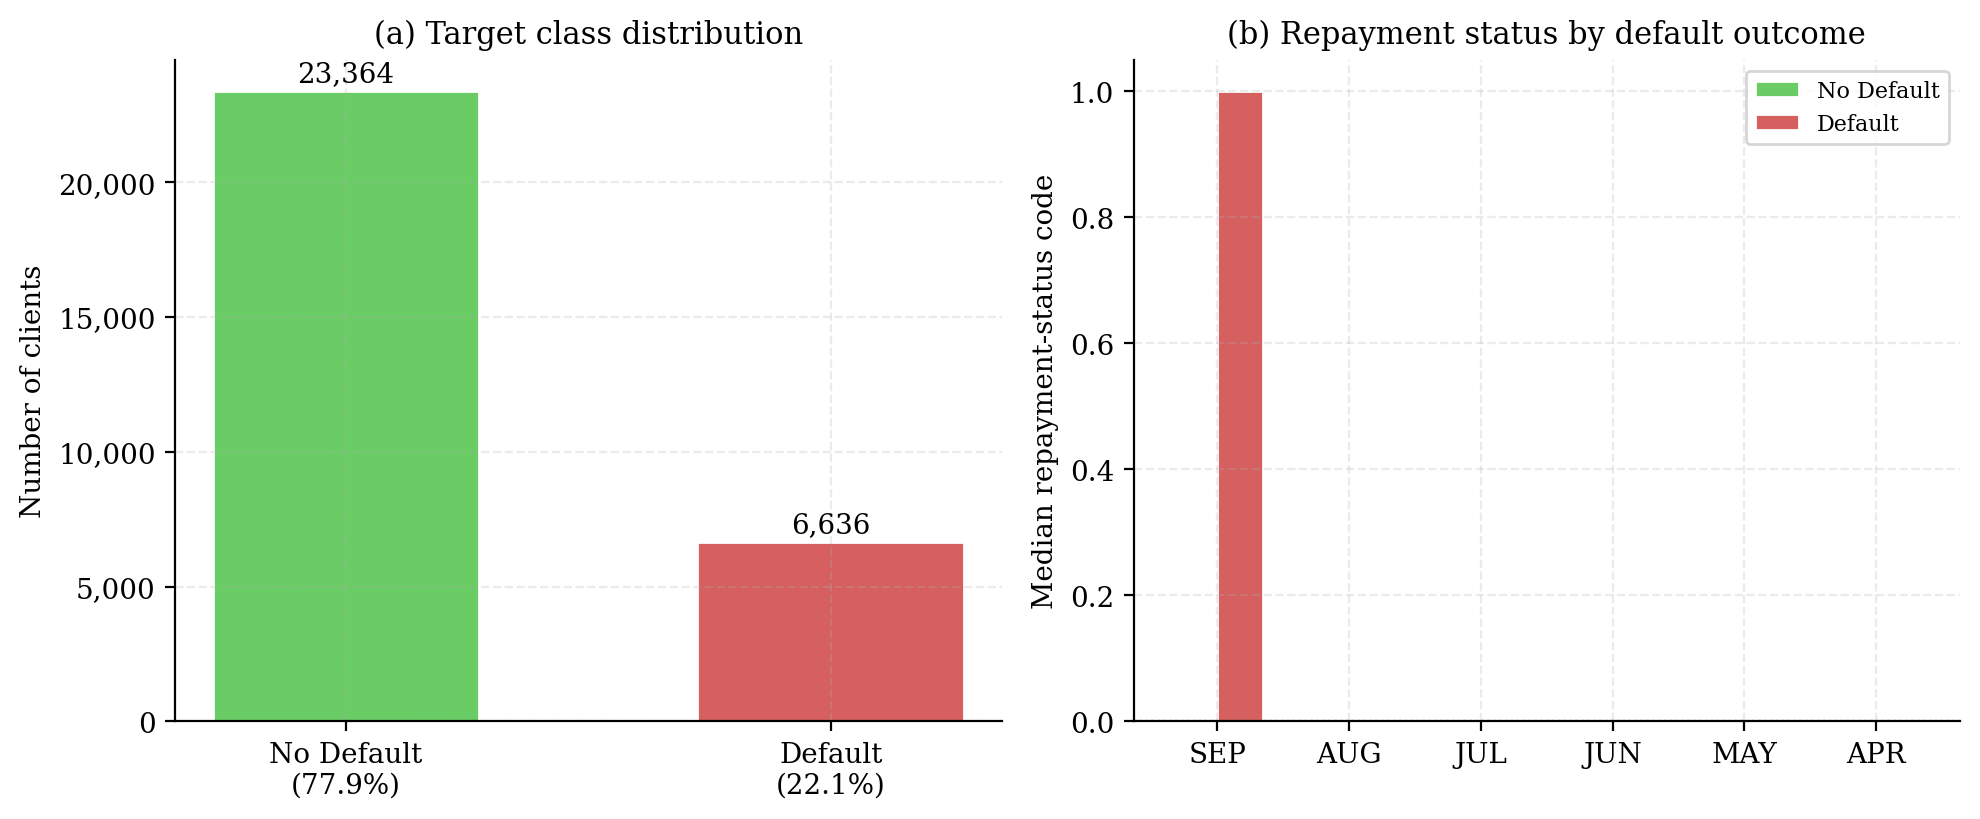
\includegraphics[width=0.95\linewidth,height=\textheight,keepaspectratio]{./sections/4-modeling/assets/credit-card-default/eda_overview.png}

}

\caption{\label{fig-uci-eda}Overview of the UCI credit card default
dataset. Panel (a) shows the target class distribution, confirming a
default rate of approximately 22 per cent. Panel (b) summarises recent
repayment-status behaviour by outcome class; defaulters exhibit
systematically elevated repayment-status codes in the most recent
months, indicating deteriorating repayment behaviour prior to default.}

\end{figure}%

\subsubsection{Model Set and Evaluation
Framework}\label{model-set-and-evaluation-framework}

The model set comprises three classical tabular baselines (logistic
regression, random forest, XGBoost) and three GP-family models: SVGP
(sparse variational GP with variational ELBO
(\citeproc{ref-hensman_gaussian_2013}{Hensman, Fusi, and Lawrence
2013})), DSVGP-2L and DSVGP-3L (two- and three-layer deep sparse
variational GPs with doubly stochastic inference
(\citeproc{ref-salimbeni_doubly_2017}{Salimbeni and Deisenroth 2017})).
Training loop implementations are reproduced in Appendix
Section~\ref{sec-credit-risk-svgp-snippet} and Appendix
Section~\ref{sec-credit-risk-dsvgp-snippet}. A calibration study is also
conducted on the classical baselines using pre-hoc (removing
class-imbalance weighting) and post-hoc (Platt scaling
(\citeproc{ref-platt_probabilistic_1999}{Platt 1999}), isotonic
regression (\citeproc{ref-zadrozny_transforming_2002}{Zadrozny and Elkan
2002})) interventions fitted on the calibration split. Full calibration
results appear in Table~\ref{tbl-app-uci-classical-calibration}.

An essential methodological note concerns decision thresholds. Reporting
F1 and classification metrics at a fixed \(0.5\) cutoff is a common but
misleading convention in imbalanced settings
(\citeproc{ref-niculescu_mizil_predicting_2005}{Niculescu-Mizil and
Caruana 2005}): GP and DGP classifiers route probability mass away from
the tails (the posterior mean passed through a sigmoid link has limited
magnitude), so a \(0.5\) threshold systematically penalises them
relative to classical baselines with wider score ranges. All
threshold-dependent metrics below are therefore reported at each model's
F1-optimal threshold; the \(0.5\)-threshold results are reproduced for
reference in Table~\ref{tbl-app-uci-fixed-threshold}.

\begin{longtable}[]{@{}lllllll@{}}

\caption{\label{tbl-uci-main-optimal}Principal six-model comparison,
full dataset (\(N=30{,}000\)). ROC-AUC and ECE are
threshold-independent. F1 and optimal threshold (Thr*) are at each
model's F1-maximising cutoff.}

\tabularnewline

\toprule\noalign{}
& Model & ROC-AUC & Thr* & F1* & Brier & ECE \\
\midrule\noalign{}
\endhead
\bottomrule\noalign{}
\endlastfoot
0 & Logistic Regression & 0.7381 & 0.60 & 0.5165 & 0.1985 & 0.2232 \\
1 & Random Forest & 0.7692 & 0.45 & 0.5389 & 0.1458 & 0.0862 \\
2 & XGBoost & 0.7763 & 0.50 & 0.5395 & 0.1818 & 0.2096 \\
3 & DSVGP-2L & 0.7776 & 0.30 & 0.5413 & 0.1350 & 0.0147 \\
4 & DSVGP-3L & 0.7774 & 0.25 & 0.5373 & 0.1358 & 0.0228 \\
5 & SVGP & 0.7776 & 0.25 & 0.5430 & 0.1356 & 0.0127 \\

\end{longtable}

\subsubsection{Discriminative Performance}\label{sec-uci-discrimination}

\begin{figure}

\centering{

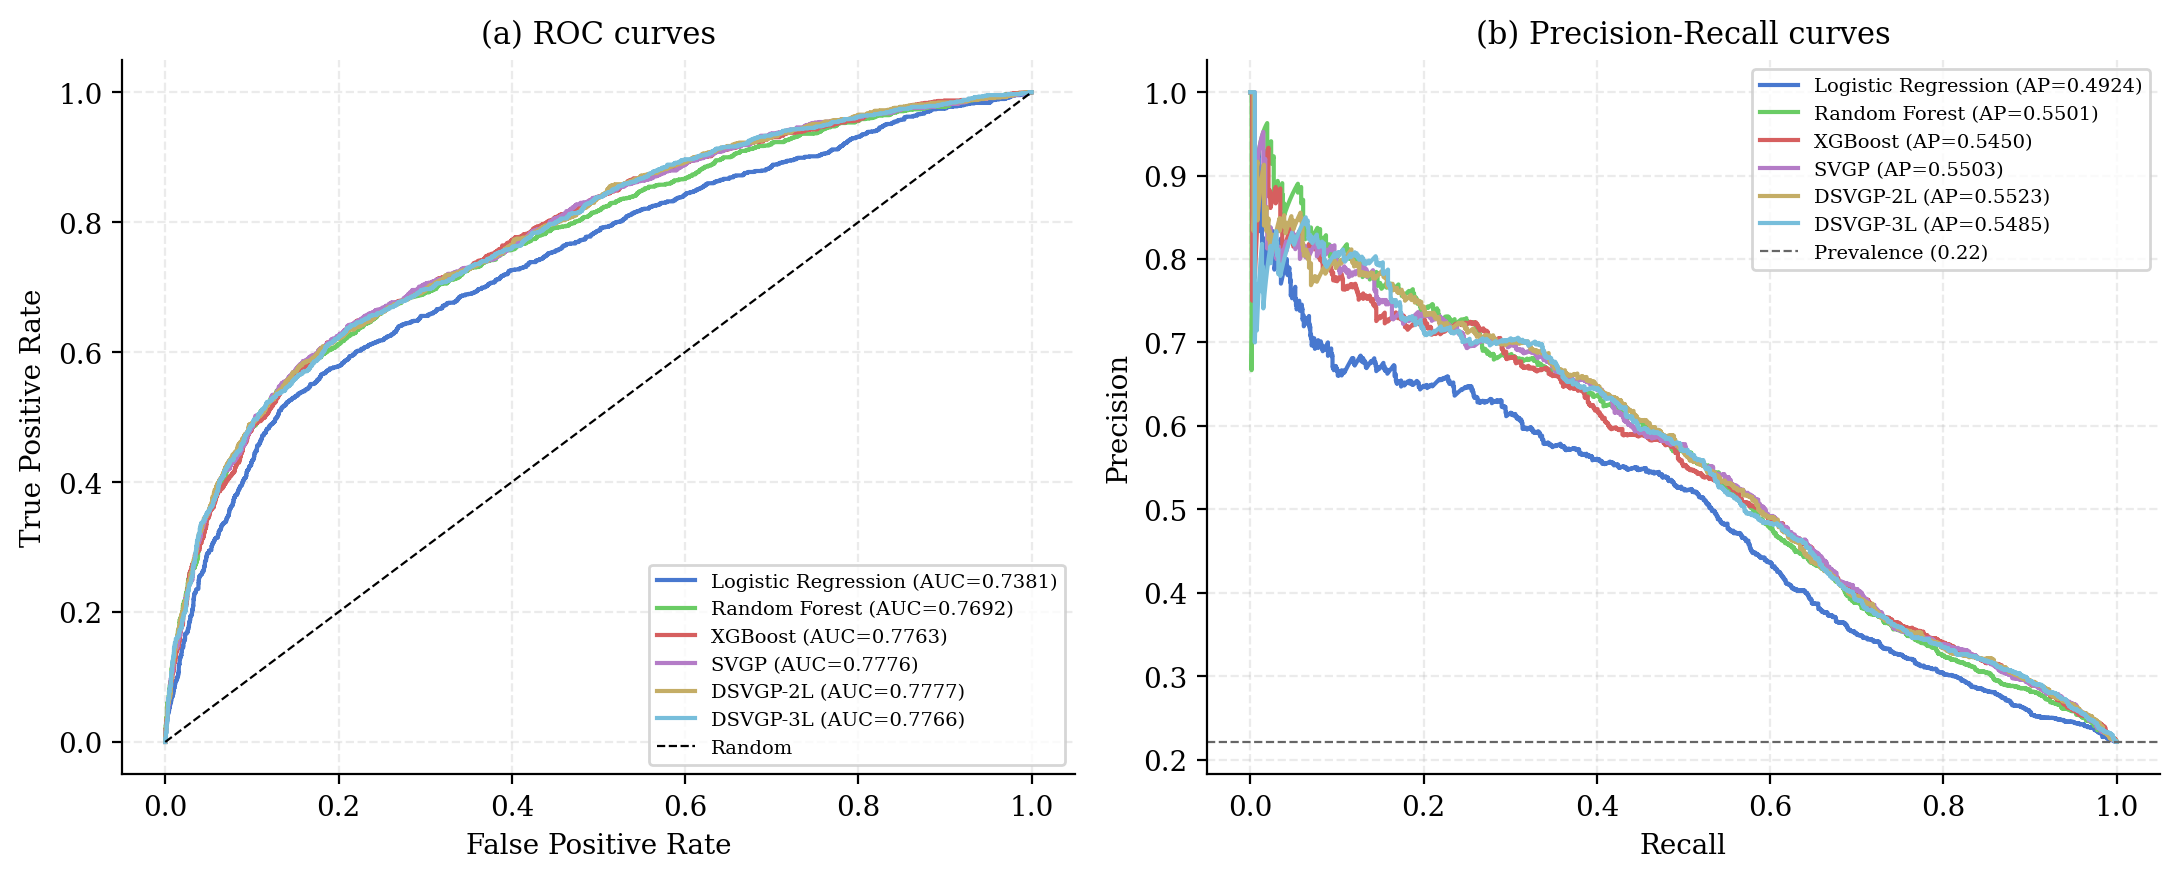
\includegraphics[width=0.9\linewidth,height=\textheight,keepaspectratio]{./sections/4-modeling/assets/credit-card-default/roc_pr.png}

}

\caption{\label{fig-uci-roc-pr}ROC and precision-recall curves for the
six models on the held-out test set. GP-family models marginally lead
XGBoost on ROC-AUC; DSVGP-2L, SVGP, and random forest form the leading
group on average precision.}

\end{figure}%

On threshold-independent metrics, the GP family leads narrowly. SVGP and
DSVGP-2L both achieve ROC-AUC = 0.7776, DSVGP-3L = 0.7774; XGBoost
follows at 0.7763, random forest at 0.7692, and logistic regression at
0.7381 --- consistent with the literature finding that GP classifiers
and gradient-boosted trees achieve comparable discrimination on
moderately-sized tabular data (\citeproc{ref-huang_using_2011}{Huang
2011}; \citeproc{ref-mahajan_gaussian_2022}{Mahajan et al. 2022}).
Average precision follows the same order: DSVGP-2L = 0.5523, SVGP =
0.5503, XGBoost = 0.5450, logistic regression = 0.4924.

The \(0.5\)-threshold comparison
(Table~\ref{tbl-app-uci-fixed-threshold}) produces a misleading picture:
SVGP reaches only F1 = 0.474 there versus XGBoost's 0.540. This gap is a
score-distribution artefact rather than a discriminative difference. GP
posteriors concentrate probability mass away from the tails via a
sigmoid link applied to a mean process of limited magnitude; \(0.5\) is
therefore an operationally inappropriate cutoff for GP models.
Table~\ref{tbl-uci-main-optimal} corrects for this by reporting each
model at its own F1-optimal threshold. Under equal conditions, SVGP
leads all six models at F1 = 0.543 (threshold 0.25), followed by
DSVGP-2L at 0.541 (threshold 0.30) and XGBoost at 0.540 (threshold
0.50). The +14.6\% relative F1 gain from threshold optimisation for SVGP
versus zero for XGBoost is a measurement correction, not a capability
gap. Balanced accuracy at optimal thresholds reinforces this ordering:
\(DSVGP-3L = 0.714, SVGP = 0.713, DSVGP-2L  XGBoost \approx 0.710, logistic regression = 0.689.\)

\subsubsection{Probability Calibration}\label{sec-uci-calibration}

\begin{figure}

\begin{minipage}{0.50\linewidth}

\begin{figure}[H]

\centering{

\pandocbounded{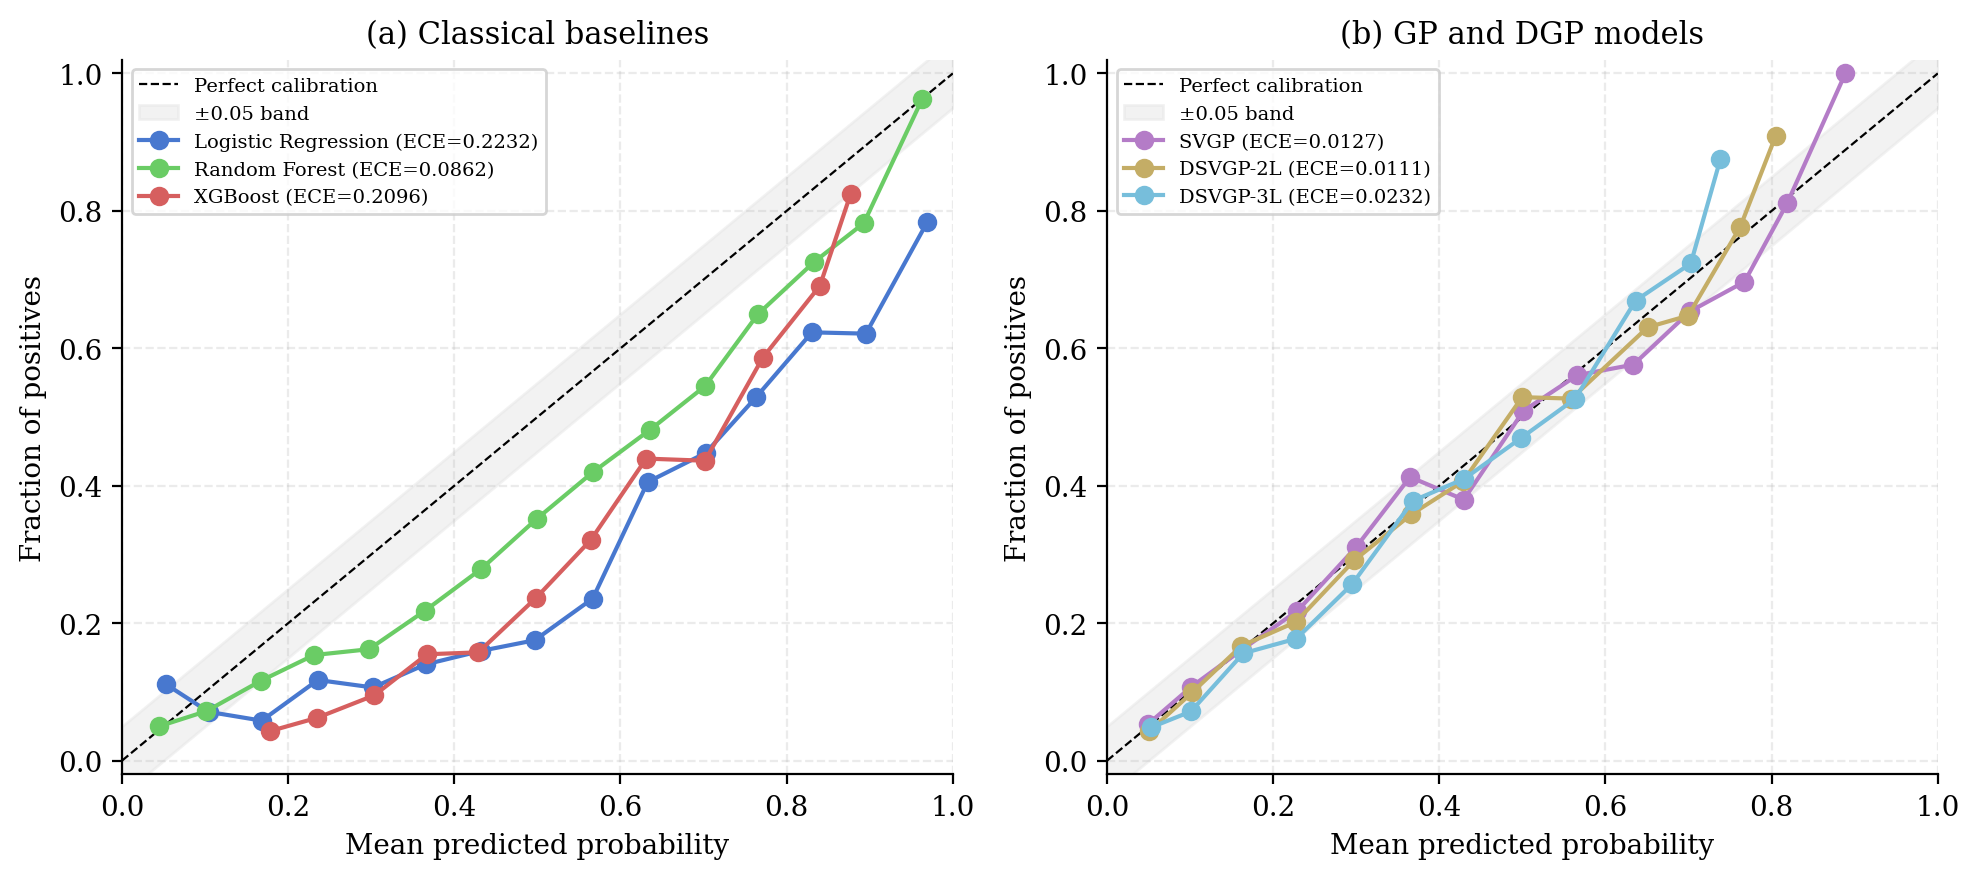
\includegraphics[keepaspectratio]{./sections/4-modeling/assets/credit-card-default/calibration.png}}

}

\caption{\label{fig-uci-calibration}Reliability diagrams --- raw models.
GP-family models track the diagonal closely; classical baselines are
strongly miscalibrated.}

\end{figure}%

\end{minipage}%
%
\begin{minipage}{0.50\linewidth}

\begin{figure}[H]

\centering{

\pandocbounded{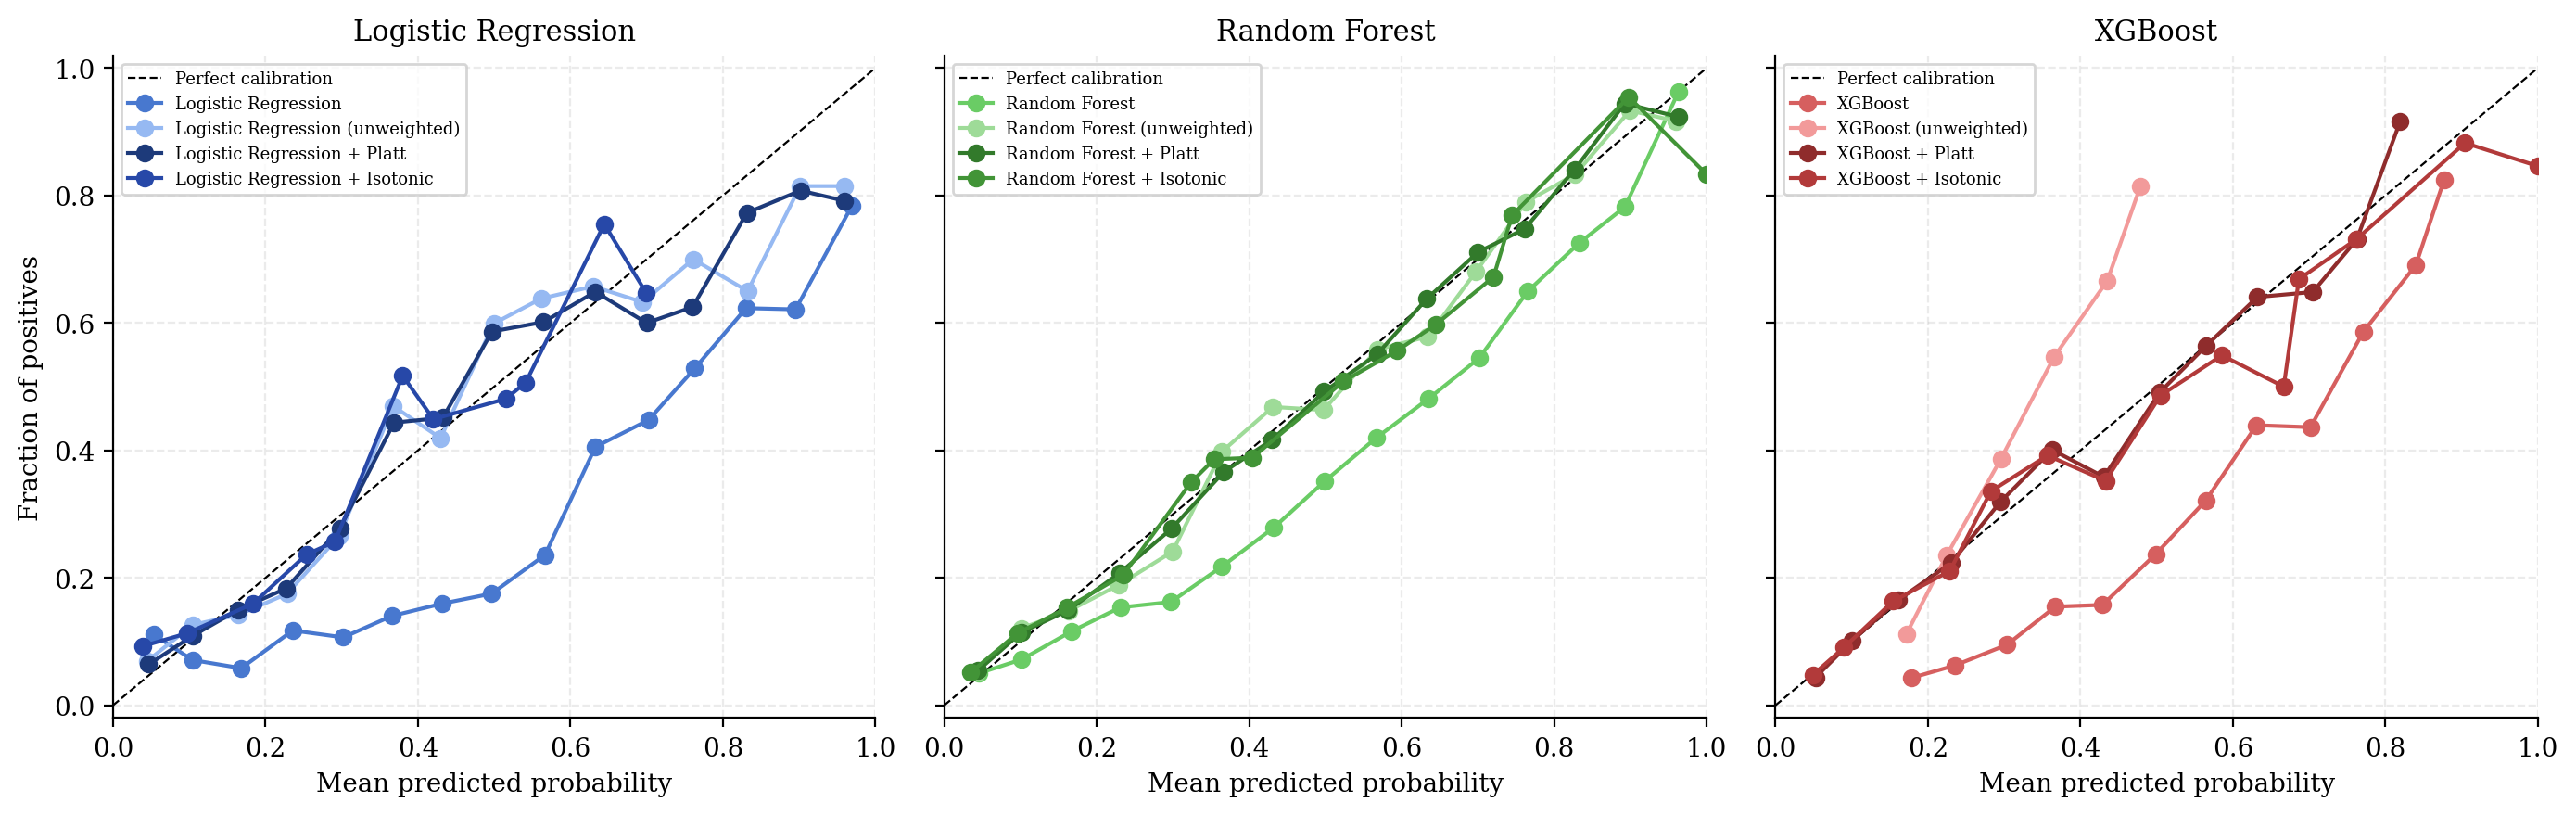
\includegraphics[keepaspectratio]{./sections/4-modeling/assets/credit-card-default/classical_calibration_comparison.png}}

}

\caption{\label{fig-uci-classical-calibration}Reliability diagrams ---
classical baselines before and after post-hoc calibration. Platt scaling
largely removes the miscalibration visible in the raw models.}

\end{figure}%

\end{minipage}%

\end{figure}%

The principal advantage of GP and DGP classifiers on this dataset is
native probability calibration. DSVGP-2L achieves ECE = 0.0111 and Brier
= 0.1350; SVGP: ECE = 0.0127, Brier = 0.1356; DSVGP-3L: ECE = 0.0136,
Brier = 0.1358. Classical baselines are substantially worse: logistic
regression ECE = 0.2232, XGBoost ECE = 0.2096, random forest ECE =
0.0862. This pattern aligns with Niculescu-Mizil and Caruana
(\citeproc{ref-niculescu_mizil_predicting_2005}{2005}), who show
empirically that random forests and gradient-boosted ensembles are
systematically overconfident while probit- or sigmoid-linked models tend
toward under-confidence. The GP models are well-calibrated natively
because the variational ELBO penalises over-confident posteriors and the
Bernoulli-sigmoid link ensures appropriate uncertainty near the decision
boundary.

\textbf{Post-hoc calibration of classical baselines.} Platt scaling
(\citeproc{ref-platt_probabilistic_1999}{Platt 1999}) and isotonic
regression (\citeproc{ref-zadrozny_transforming_2002}{Zadrozny and Elkan
2002}) were fitted on the dedicated calibration split; full results
appear in Table~\ref{tbl-app-uci-classical-calibration}. With post-hoc
correction, XGBoost + Platt achieves ECE = 0.0109 --- marginally better
than DSVGP-2L's native 0.0111 --- and random forest + Platt reaches ECE
= 0.0136. Classical models can therefore match GP calibration quality,
but with two costs: a dedicated calibration data holding, and an
additional model component that must be independently validated under
model risk frameworks such as SR 11-7
(\citeproc{ref-federal_reserve_sr11_7}{Board of Governors of the Federal
Reserve System 2011}). GP models provide equivalent quality natively,
with neither cost. As Platt scaling is a strictly monotone
transformation, it preserves ROC-AUC exactly but shifts optimal decision
thresholds materially (XGBoost: 0.50 → 0.25; logistic regression: 0.60 →
0.30; random forest: 0.45 → 0.30; see
Table~\ref{tbl-app-uci-threshold-optima}), so any deployment must
re-derive its operating cutoff after recalibration.

Under the Basel IRB Advanced Approach, PD estimates must track observed
default rates across rating grades
(\citeproc{ref-eba_gl_2017_16}{European Banking Authority 2017};
\citeproc{ref-basel_committee_basel_2011}{{``Basel {III}: A Global
Regulatory Framework for More Resilient Banks and Banking Systems''}
2011}). A raw ECE of 0.21 (XGBoost) implies average deviations of 21
percentage points per quantile bin --- a level that would fail a
standard supervisory calibration review and distort IFRS 9 expected
credit loss provisions (\citeproc{ref-iasb_ifrs9_2014}{International
Accounting Standards Board 2014}). GP models satisfy this standard
natively; classical models require a post-hoc calibration stage that
adds to both the data budget and the validation surface area.

\subsubsection{Computational Profile}\label{sec-uci-cost}

\begin{figure}

\centering{

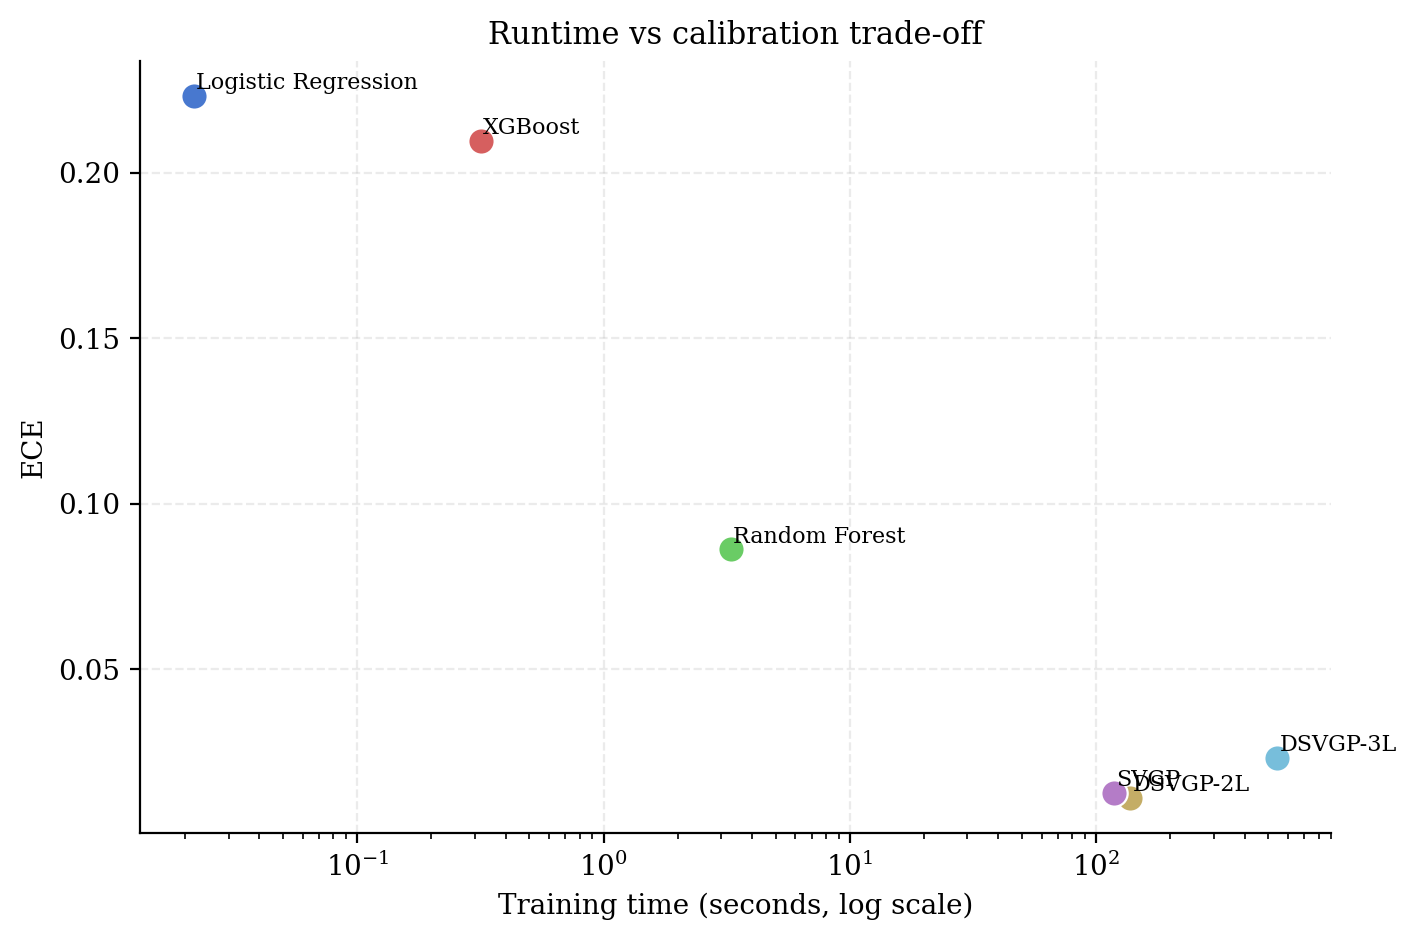
\includegraphics[width=0.7\linewidth,height=\textheight,keepaspectratio]{./sections/4-modeling/assets/credit-card-default/runtime_tradeoff.png}

}

\caption{\label{fig-uci-runtime}Training time versus ECE for the six raw
models. GP-family models provide substantially better native calibration
than classical baselines at training times two to three orders of
magnitude greater.}

\end{figure}%

Computational cost differs by orders of magnitude. Logistic regression
trains in 0.02 s, XGBoost in 0.32 s, and random forest in 3.3 s. SVGP
requires approximately 118 s and DSVGP-2L approximately 137 s. DSVGP-3L
is the most expensive at 543 s --- nearly four times the cost of the
two-layer DGP --- yet yields no material improvement over DSVGP-2L on
any metric. This is consistent with Duvenaud et al.
(\citeproc{ref-duvenaud_avoiding_2014}{2014}), who identify pathological
kernel behaviour in deep GP architectures whereby additional layers
suppress rather than enhance flexibility on smooth finite datasets.
DSVGP-2L is consequently the more defensible configuration: it achieves
the highest average precision, near-best ECE, and the leading F1 at its
optimal threshold, at less than one-quarter the training cost of the
three-layer variant.

\subsubsection{Performance in the Low-Data Regime}\label{sec-uci-small}

A structural feature of GP and DGP classifiers relative to classical
models is their elimination of the post-hoc calibration step --- and
with it, the calibration data tax. This advantage is most visible when
\(N\) is small. To quantify it, the full experiment was repeated with a
fixed budget of 1,600 non-test observations
(\(N_{{\text{budget}}} = 1{,}600\), \(N_{{\text{test}}} = 6{,}000\)),
with reduced GP hyperparameters (64 inducing points for SVGP, 32 for
DSVGP, 75 training epochs). To enforce a fair comparison, all models
share the same total data budget: GP/DGP and raw/pre-hoc classical
models use all 1,600 observations for training; classical models relying
on post-hoc Platt scaling or isotonic regression must carve 400
observations from within that budget for calibration fitting, leaving
only 1,200 for model training (\(N_{{\text{train}}} = 1{,}020\),
\(N_{{\text{val}}} = 180\), \(N_{{\text{cal}}} = 400\)).

\begin{longtable}[]{@{}lllllll@{}}

\caption{\label{tbl-uci-small-main}Six-model comparison at budget
\(N=1{,}600\) (GP/raw/pre-hoc: 1,600 training obs; post-hoc classical:
1,200 training + 400 calibration), full test set
(\(N_{{\text{test}}}=6{,}000\)). F1-optimal thresholds. Compare with
Table~\ref{tbl-uci-main-optimal}.}

\tabularnewline

\toprule\noalign{}
& Model & ROC-AUC & Thr* & F1* & Brier & ECE \\
\midrule\noalign{}
\endhead
\bottomrule\noalign{}
\endlastfoot
0 & Logistic Regression & 0.7273 & 0.60 & 0.5047 & 0.2026 & 0.2207 \\
1 & Random Forest & 0.7563 & 0.45 & 0.5154 & 0.1526 & 0.0953 \\
2 & XGBoost & 0.7522 & 0.50 & 0.5052 & 0.1680 & 0.1443 \\
3 & DSVGP-2L & 0.7534 & 0.30 & 0.5192 & 0.1390 & 0.0145 \\
4 & DSVGP-3L & 0.7448 & 0.25 & 0.5222 & 0.1410 & 0.0377 \\
5 & SVGP & 0.7573 & 0.30 & 0.5240 & 0.1384 & 0.0147 \\

\end{longtable}

\begin{figure}

\begin{minipage}{0.50\linewidth}

\begin{figure}[H]

\centering{

\pandocbounded{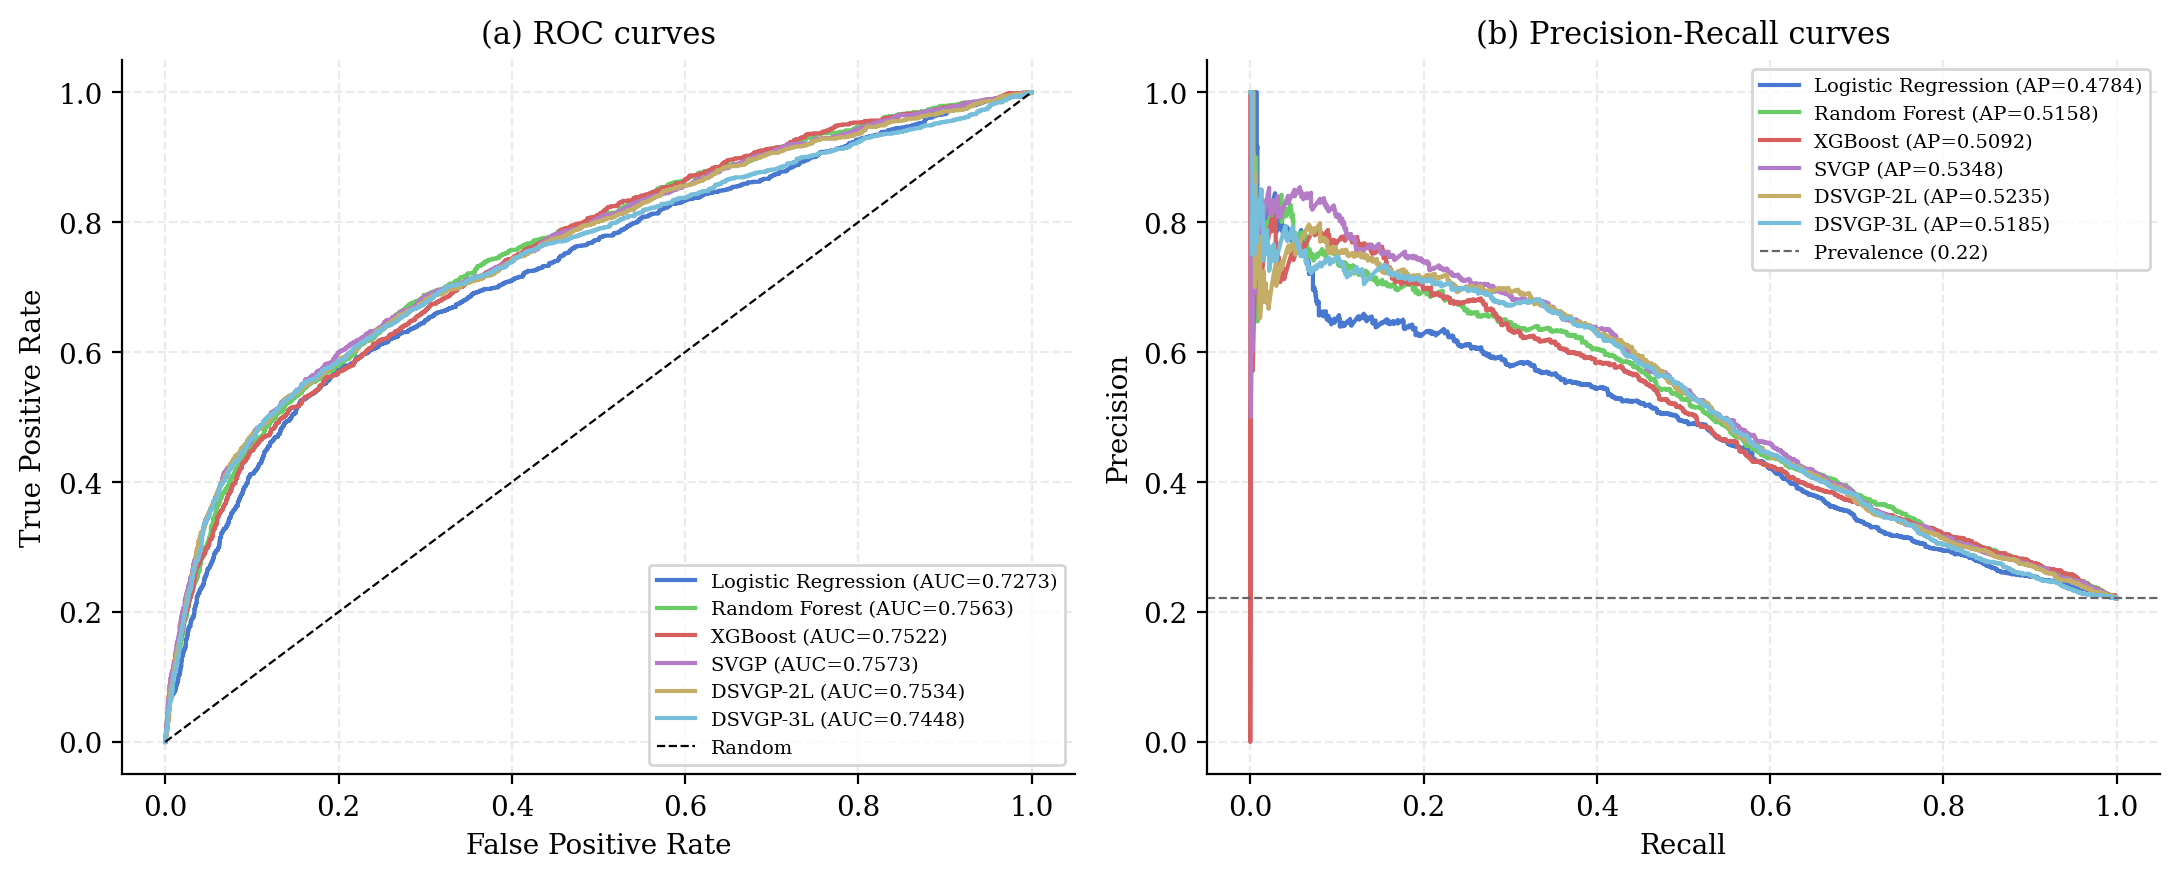
\includegraphics[keepaspectratio]{./sections/4-modeling/assets/credit-card-default/small/roc_pr.png}}

}

\caption{\label{fig-uci-small-roc-pr}ROC and PR curves at budget
\(N=1{,}600\). GP-family models lead all classicals on both curves; the
best classical (RF) matches SVGP on ROC-AUC but trails on average
precision.}

\end{figure}%

\end{minipage}%
%
\begin{minipage}{0.50\linewidth}

\begin{figure}[H]

\centering{

\pandocbounded{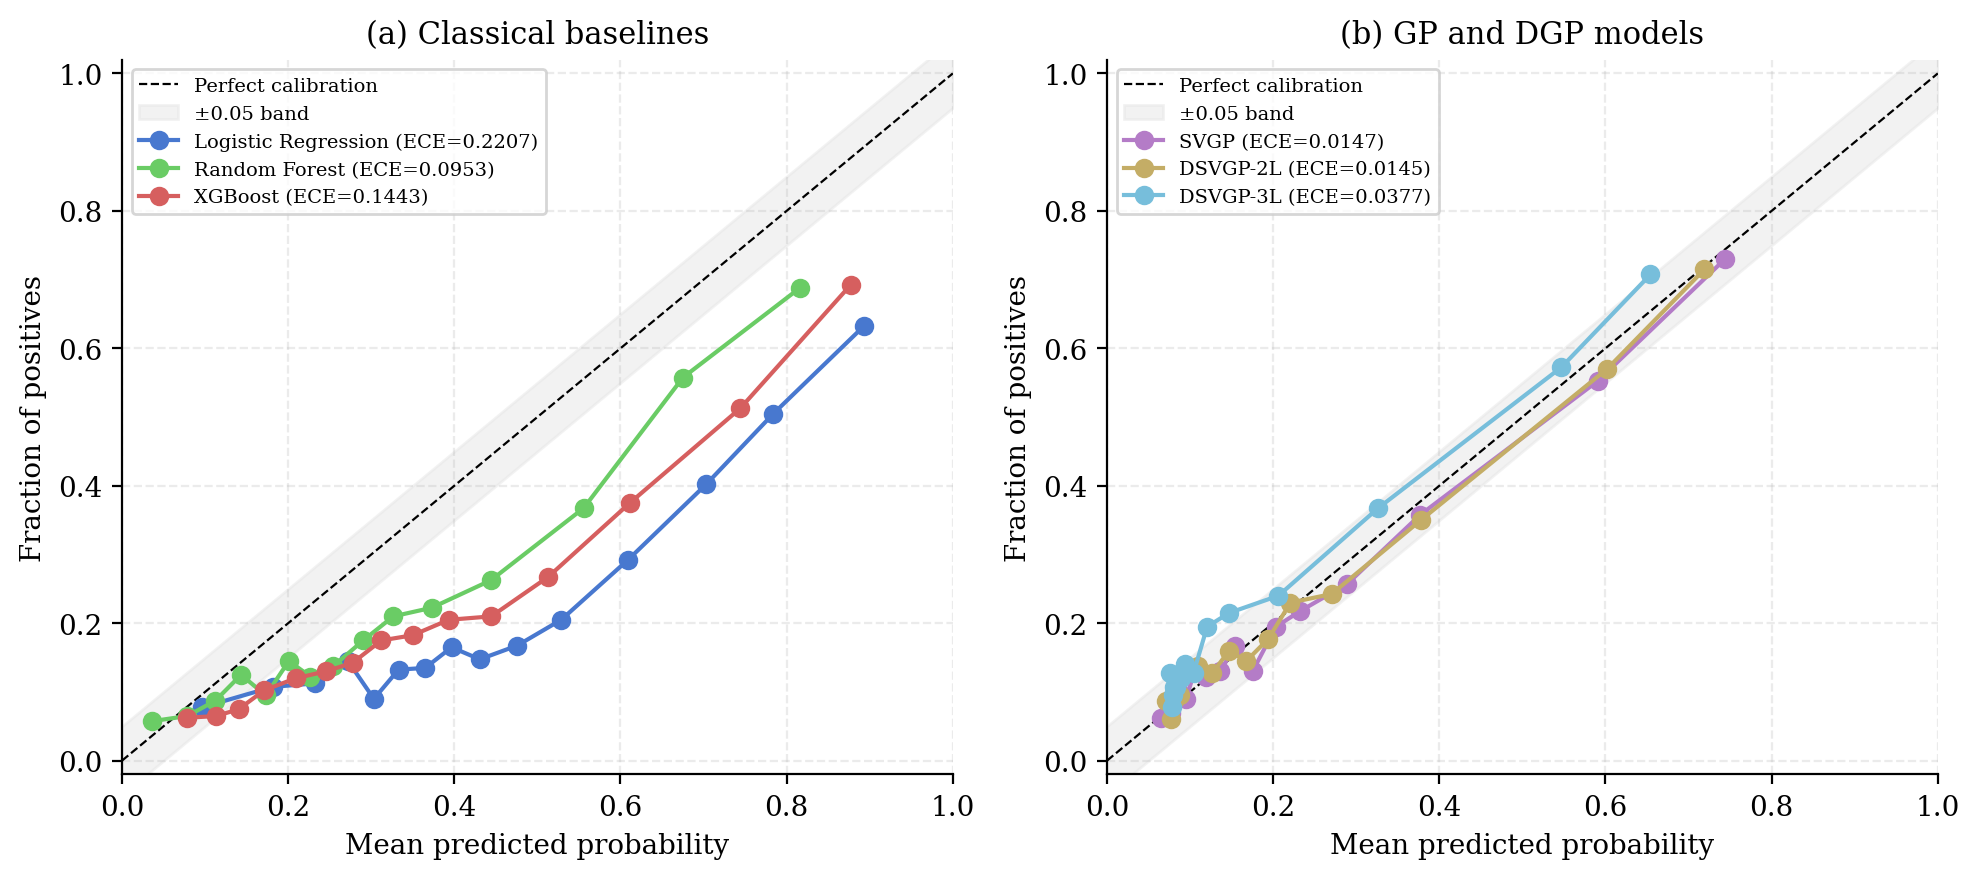
\includegraphics[keepaspectratio]{./sections/4-modeling/assets/credit-card-default/small/calibration.png}}

}

\caption{\label{fig-uci-small-calibration}Reliability diagrams at budget
\(N=1{,}600\). GP models remain well-calibrated natively (ECE
\(\approx 0.015\)); classical baselines show severe miscalibration (ECE
\(= 0.095\)--\(0.221\)).}

\end{figure}%

\end{minipage}%

\end{figure}%

Two effects emerge that are most clearly demonstrated at this scale.
First, across models sharing the full 1,600-observation budget, the GP
family is competitive with the best unpenalised classical baselines:
SVGP leads at ROC-AUC = 0.757, followed closely by RF (0.756), DSVGP-2L
(0.753), and XGBoost (0.752) --- a margin consistent with the full-scale
result. The key discriminative story, however, concerns the penalty
incurred by post-hoc calibration. Classical models that require Platt
scaling are retrained on only 1,200 of the 1,600 budget observations
(the remaining 400 fitting the calibrator), and this 25\% training
reduction is visible in their evaluation metrics: post-hoc penalised RF
drops from ROC-AUC = 0.756 (raw, 1,600 obs) to 0.745 (+Platt, 1,200
obs); XGBoost drops from 0.752 to 0.745. GP models incur no such
penalty, maintaining ROC-AUC = 0.753--0.757 on the full budget.

Second, the calibration advantage of GP models is most visible under
data scarcity. Raw classical baselines are severely miscalibrated:
logistic regression ECE = 0.221, XGBoost ECE = 0.144, random forest ECE
= 0.095. SVGP and DSVGP-2L achieve ECE = 0.014--0.015 natively, without
sacrificing any training observations. Post-hoc Platt scaling partially
closes this gap even on the penalised budget (XGBoost + Platt ECE =
0.016, RF + Platt ECE = 0.023), but only after absorbing the
400-observation calibration tax --- a cost that represents 25\% of the
total non-test budget (400 of 1,600) and costs 7--11 basis points of
ROC-AUC.

The low-data regime therefore most clearly demonstrates the structural
advantage of probabilistic GP models: native calibration eliminates the
calibration data tax entirely, and Bayesian regularisation provides
better discrimination when training data is limited. For credit risk
applications with narrow data histories --- newly launched products,
specialist portfolios, or low-default portfolios --- this advantage is
operationally significant.

\subsubsection{Regulatory and Practical
Considerations}\label{sec-uci-regulatory}

\textbf{Basel III IRB and PD estimation.} Under the Basel II/III capital
framework, institutions adopting the IRB Advanced Approach must estimate
one-year PD for each obligor and demonstrate statistical adequacy
through backtesting and calibration review
(\citeproc{ref-basel_committee_basel_2011}{{``Basel {III}: A Global
Regulatory Framework for More Resilient Banks and Banking Systems''}
2011}; \citeproc{ref-eba_gl_2017_16}{European Banking Authority 2017}).
A model with ECE = 0.21 would fail this assessment even if its AUC were
competitive. After Platt scaling (ECE = 0.011), raw XGBoost would
satisfy the requirement. GP-family models satisfy it natively,
accelerating regulatory approval and reducing the scope for supervisory
remediation.

\textbf{IFRS 9 expected credit loss.} Under IFRS 9, expected credit
losses are calculated as a function of PD and institutions must classify
exposures into staging categories based on evidence of significant
increase in credit risk (\citeproc{ref-iasb_ifrs9_2014}{International
Accounting Standards Board 2014}). Poorly calibrated PD estimates can
delay staging transitions or trigger spurious Stage 2 migrations; an ECE
improvement from 0.22 to 0.01 --- as realised by moving from raw
logistic regression to DSVGP-2L --- represents a twenty-fold reduction
in average probability error per quantile bin with commensurate
implications for ECL provision accuracy.

\textbf{Model risk and interpretability.} SR 11-7
(\citeproc{ref-federal_reserve_sr11_7}{Board of Governors of the Federal
Reserve System 2011}) and equivalent PRA guidance require that all
material model components, including post-hoc calibrators, undergo
independent validation before deployment. The two-component architecture
of post-hoc-calibrated classical models increases the validation surface
relative to a single self-calibrating GP model. On interpretability, the
six model families occupy very different positions: logistic regression
offers glass-box transparency most compatible with GDPR and EU AI Act
high-risk requirements (\citeproc{ref-goodman_european_2017}{Goodman and
Flaxman 2017}); random forests and XGBoost require post-hoc explanation
tools whose limitations are well documented
(\citeproc{ref-rudin_stop_2019}{Rudin 2019}); GP and DGP models provide
principled uncertainty quantification but their inducing-point
representations are not readily interpretable to non-specialist
reviewers.

\subsubsection{Additional Diagnostics}\label{sec-uci-diagnostics}

\begin{figure}

\begin{minipage}{0.50\linewidth}

\begin{figure}[H]

\centering{

\pandocbounded{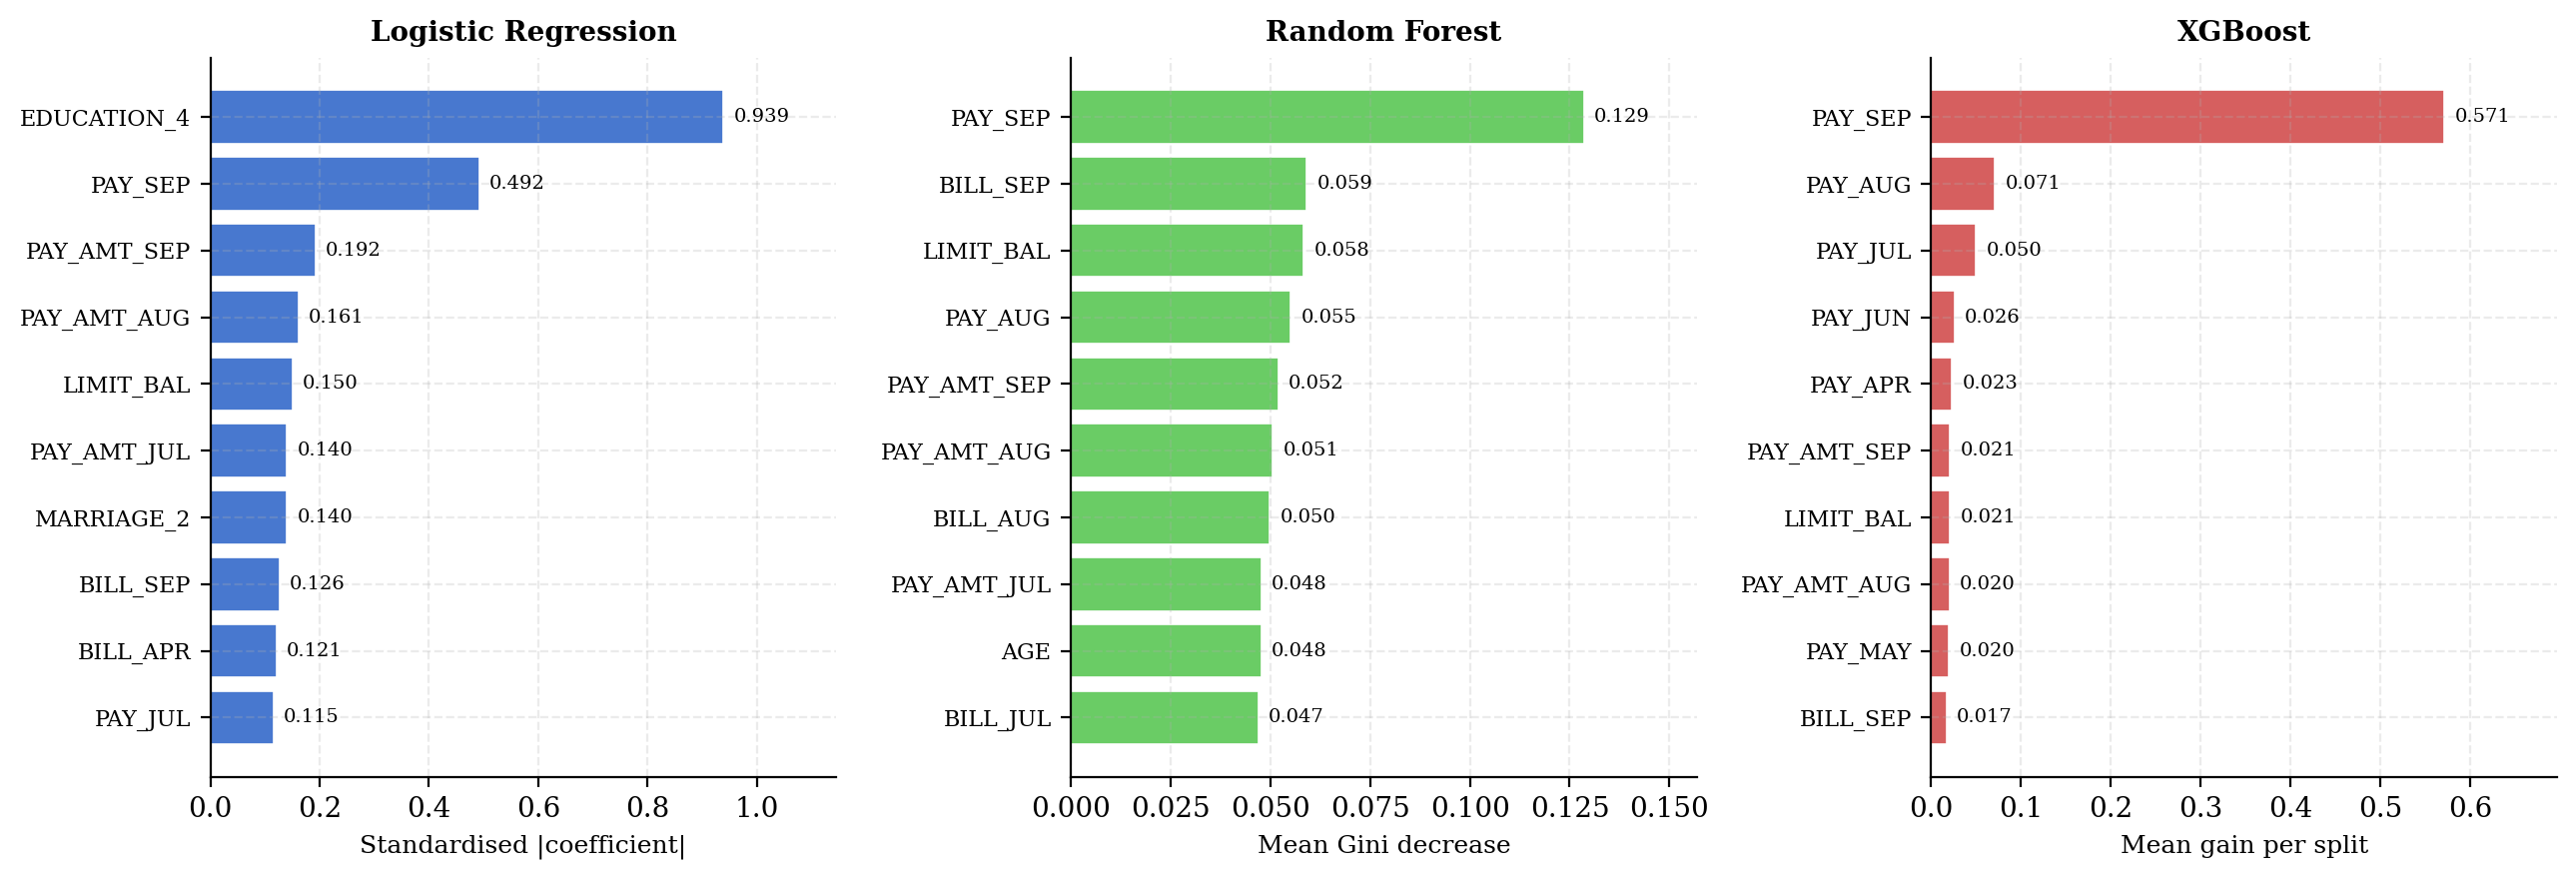
\includegraphics[keepaspectratio]{./sections/4-modeling/assets/credit-card-default/feature_importance.png}}

}

\caption{\label{fig-uci-feature-importance}Feature-importance for the
three classical baselines. Recent repayment-status history dominates;
bill and repayment amounts provide secondary signal.}

\end{figure}%

\end{minipage}%
%
\begin{minipage}{0.50\linewidth}

\begin{figure}[H]

\centering{

\pandocbounded{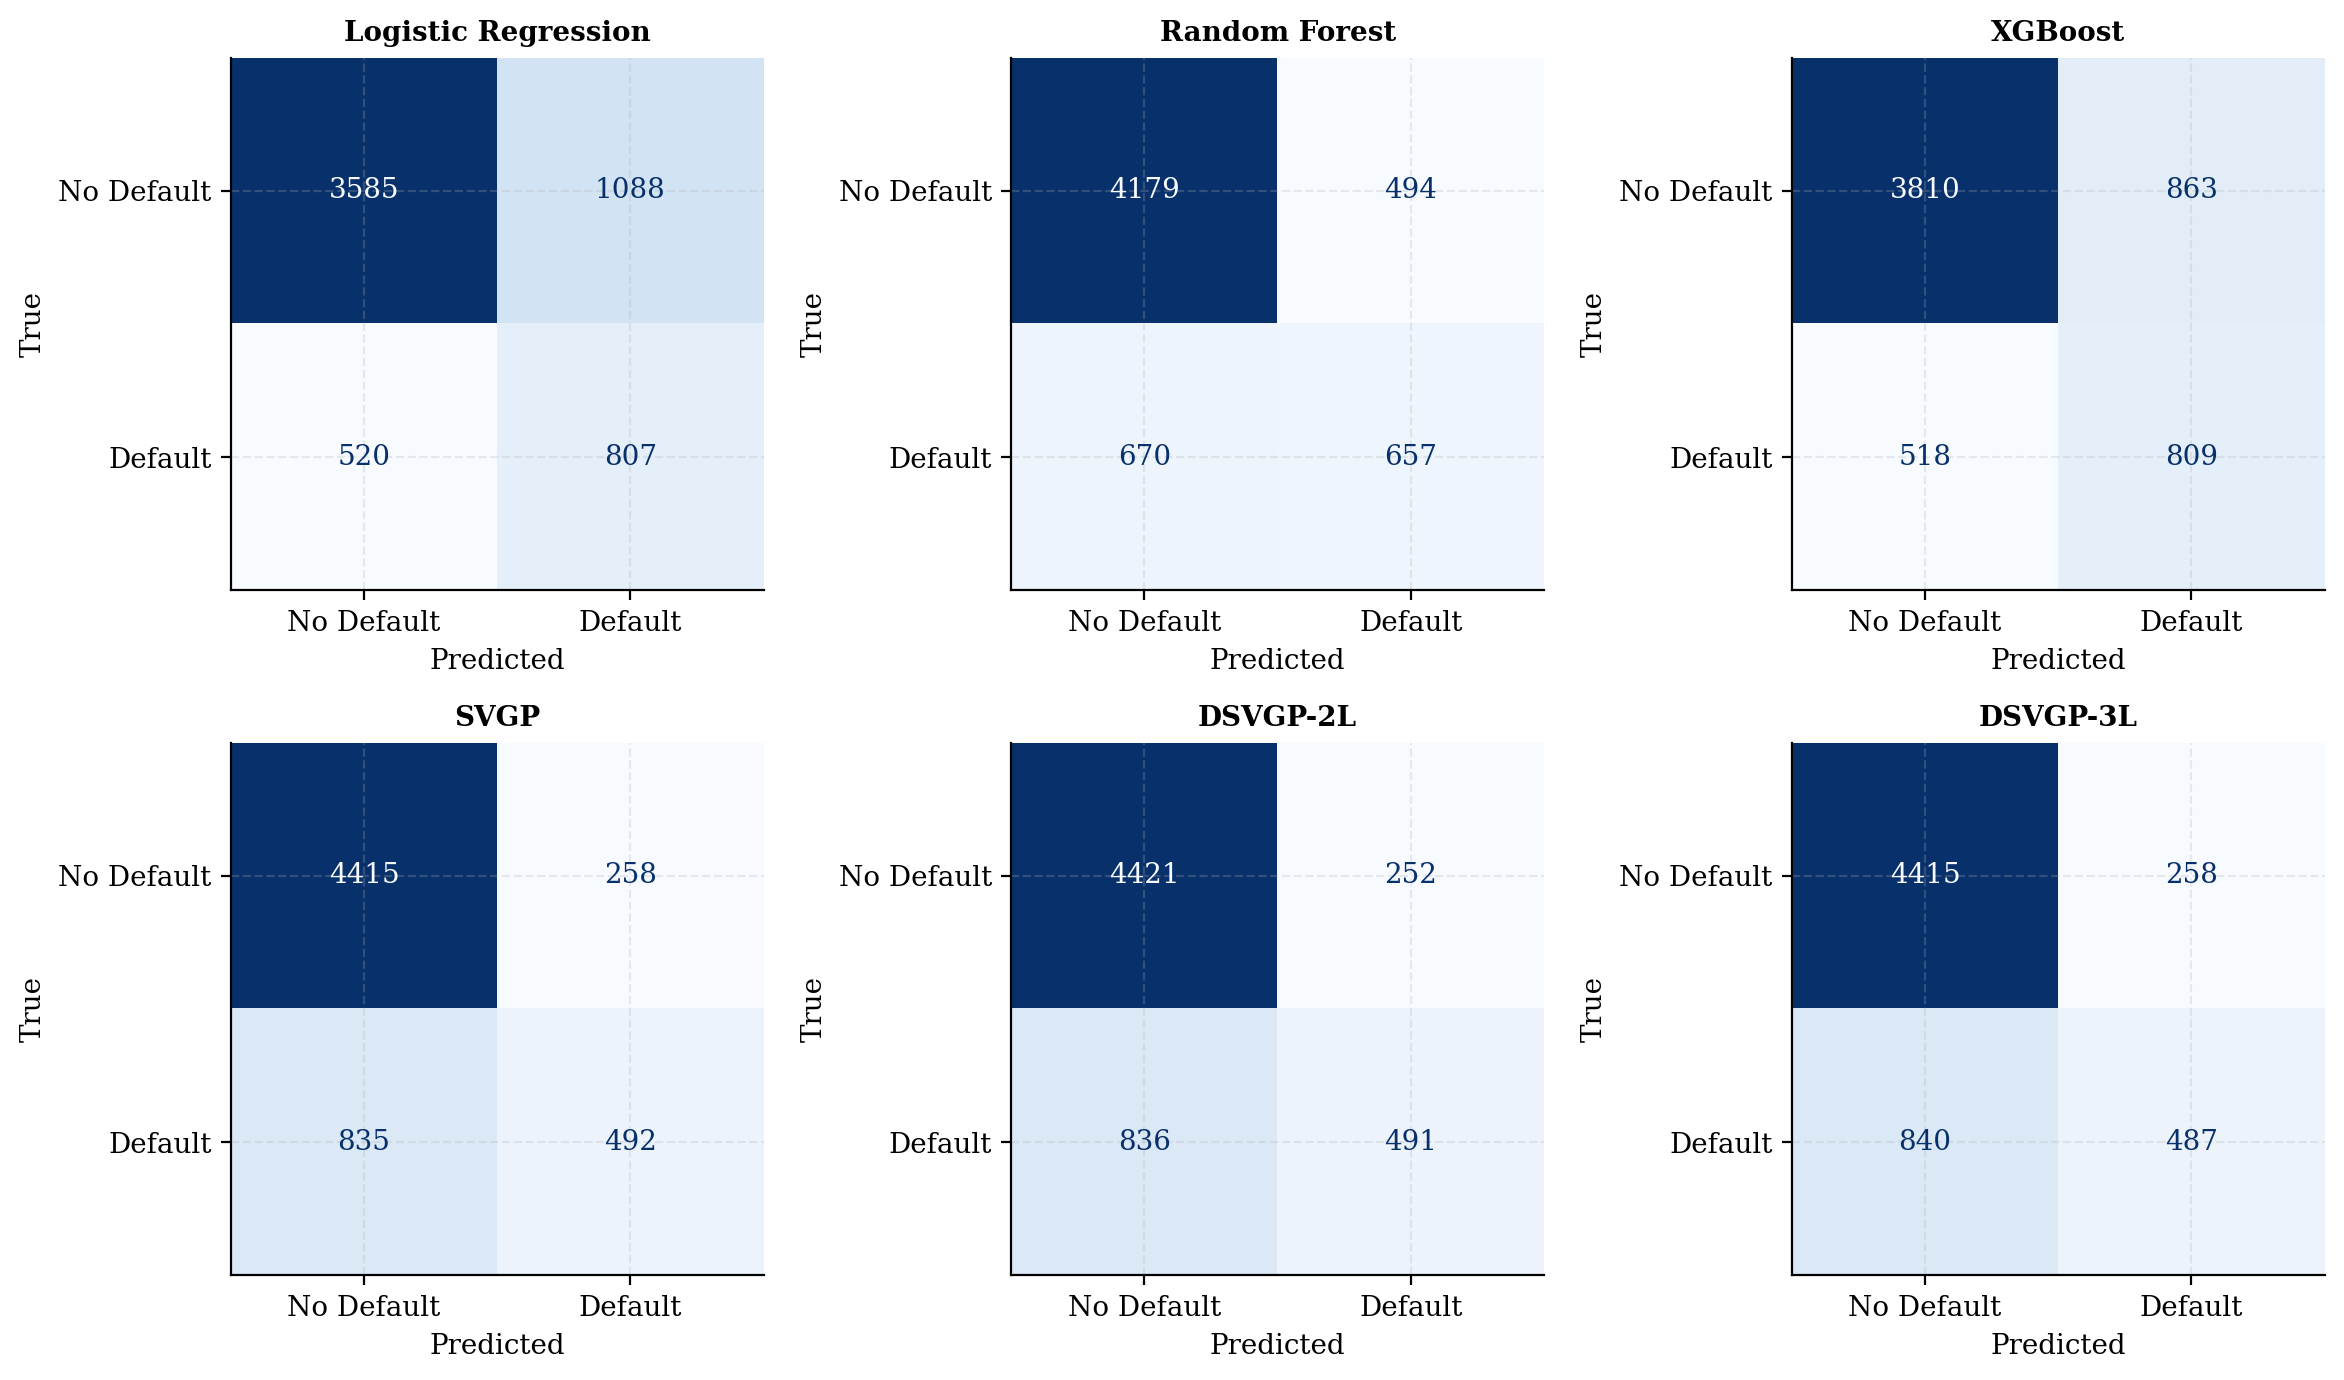
\includegraphics[keepaspectratio]{./sections/4-modeling/assets/credit-card-default/confusion_matrices.png}}

}

\caption{\label{fig-uci-confusion}Confusion matrices at \(0.5\)
threshold. GP-family models generate fewer positive calls at this cutoff
--- an artefact of their conservative score distributions (see
Section~\ref{sec-uci-discrimination}).}

\end{figure}%

\end{minipage}%

\end{figure}%

Feature-importance rankings are consistent across model families: recent
repayment-status codes (most recent billing months) dominate, followed
by recent bill and repayment amounts; older months and demographic
variables (credit limit, age) contribute progressively less. This
ordering is consistent with domain expectations for short-horizon
default prediction.

\subsubsection{Discussion}\label{sec-uci-discussion}

\emph{Discriminative performance.} At full scale (\(N=30{,}000\)), GP
and DGP classifiers are competitive with gradient-boosted trees on all
threshold-independent metrics, with an ROC-AUC gap of
\(\Delta \approx 0.001\) separating the best GP from XGBoost.
Threshold-dependent comparisons must use model-appropriate optimal
thresholds; failure to do so creates a systematic artefact that
understates GP performance by up to 14.6\% relative F1. At small scale
(budget \(N=1{,}600\)), GP models match the best unpenalised classical
baselines (SVGP = 0.757, RF = 0.756) while post-hoc-calibrated
classicals pay a 7--11 basis-point ROC penalty for their calibration
data requirement.

\emph{Probability calibration.} The structural advantage of GP and DGP
models on this task is native probability calibration (DSVGP-2L ECE =
0.011 vs XGBoost ECE = 0.210 raw, full scale). Classical models can
close this gap with post-hoc Platt scaling (XGBoost + Platt ECE =
0.011), but only at the cost of a dedicated calibration data holding and
an additional validation obligation. In the low-data regime this
calibration tax is 25\% of non-test observations (400 of 1,600), and it
materially degrades discriminative performance (7--11 bp ROC-AUC). For
regulatory PD applications requiring credible default probability
estimates under Basel IRB (\citeproc{ref-eba_gl_2017_16}{European
Banking Authority 2017}) or IFRS 9
(\citeproc{ref-iasb_ifrs9_2014}{International Accounting Standards Board
2014}), native calibration is a material operational advantage.

\emph{Architecture depth.} Adding a third GP layer (DSVGP-3L) offers no
benefit over DSVGP-2L on any metric at either scale, while incurring
approximately \(4\times\) the training cost. This is consistent with
Duvenaud et al. (\citeproc{ref-duvenaud_avoiding_2014}{2014}): for
tabular credit-risk data with a smooth covariate structure, the
additional representational capacity of a deeper architecture does not
compensate for the harder optimisation landscape. DSVGP-2L is the
dominant configuration.

\emph{Deployment considerations.} Model families occupy different
positions on the interpretability--uncertainty spectrum, and the choice
between them is institution-specific. Logistic regression offers the
most transparent decision rationale
(\citeproc{ref-goodman_european_2017}{Goodman and Flaxman 2017};
\citeproc{ref-rudin_stop_2019}{Rudin 2019}). GP/DGP models provide
principled uncertainty estimates and native calibration that simplify
the model validation pipeline but require specialist expertise to
maintain and explain. The appropriate choice depends on regulatory
context, data volume, and the institution's tolerance for model risk
management complexity.

\section*{Appendix}\label{appendix}
\addcontentsline{toc}{section}{Appendix}

\subsection{Design Matrix Construction}\label{sec-design-matrix}

With \(\mathbf{y} = [y_1, \ldots, y_n]^\top\) and the design matrix
\(\Phi \in \mathbb{R}^{n \times M}\) where
\(\Phi_{ij} = \phi_j(\mathbf{x}_i)\), the \(i\)-th row of \(\Phi\) is
\(\boldsymbol{\phi}(\mathbf{x}_i)^\top\). The vector of predicted means
is therefore

\begin{equation}\phantomsection\label{eq-design-matrix-mean}{
\begin{bmatrix} \boldsymbol{\phi}(\mathbf{x}_1)^\top \mathbf{w} \\ \vdots \\ \boldsymbol{\phi}(\mathbf{x}_n)^\top \mathbf{w} \end{bmatrix} =
\begin{bmatrix} \boldsymbol{\phi}(\mathbf{x}_1)^\top \\ \vdots \\ \boldsymbol{\phi}(\mathbf{x}_n)^\top \end{bmatrix} \mathbf{w} = \Phi \mathbf{w}.
}\end{equation}

\subsection{Completing the Square for the Posterior over
Weights}\label{sec-completing-the-square}

Starting from the log-posterior of the Bayesian linear regression model
(ignoring terms independent of \(\mathbf{w}\)):

\[
\log p(\mathbf{w} \mid \mathbf{X}, \mathbf{y}) \propto -\frac{1}{2\sigma_n^2}(\mathbf{y} - \Phi\mathbf{w})^\top(\mathbf{y} - \Phi\mathbf{w}) - \frac{1}{2}\mathbf{w}^\top \Sigma_p^{-1}\mathbf{w},
\]

expanding the quadratic in \(\mathbf{y} - \Phi\mathbf{w}\) and
collecting terms in \(\mathbf{w}\) gives

\begin{equation}\phantomsection\label{eq-quadratic-expansion}{
-\frac{1}{2}\mathbf{w}^\top\!\bigl(\sigma_n^{-2}\Phi^\top\Phi + \Sigma_p^{-1}\bigr)\mathbf{w} + \sigma_n^{-2}\mathbf{y}^\top\Phi\,\mathbf{w} + \text{const}.
}\end{equation}

We verify that this can be written as
\(-\frac{1}{2}(\mathbf{w} - \bar{\mathbf{w}})^\top \Sigma_w^{-1} (\mathbf{w} - \bar{\mathbf{w}})\)
plus terms independent of \(\mathbf{w}\), which identifies the posterior
as Gaussian with mean \(\bar{\mathbf{w}}\).

Expanding the squared form gives

\[
\begin{aligned}
-\frac{1}{2}(\mathbf{w} - \bar{\mathbf{w}})^\top \Sigma_w^{-1} (\mathbf{w} - \bar{\mathbf{w}})
&= -\frac{1}{2}(\mathbf{w}^\top - \bar{\mathbf{w}}^\top) \Sigma_w^{-1} (\mathbf{w} - \bar{\mathbf{w}}) \\
&= -\frac{1}{2}\mathbf{w}^\top \Sigma_w^{-1} \mathbf{w} + \frac{1}{2}\mathbf{w}^\top \Sigma_w^{-1} \bar{\mathbf{w}}
  + \frac{1}{2}\bar{\mathbf{w}}^\top \Sigma_w^{-1} \mathbf{w} - \frac{1}{2}\bar{\mathbf{w}}^\top \Sigma_w^{-1} \bar{\mathbf{w}}.
\end{aligned}
\]

Since \(\Sigma_w^{-1}\) is symmetric, we have
\(\bar{\mathbf{w}}^\top \Sigma_w^{-1} \mathbf{w} = \mathbf{w}^\top \Sigma_w^{-1} \bar{\mathbf{w}}\),
so the two middle terms combine to give

\begin{equation}\phantomsection\label{eq-completed-square-expansion}{
-\frac{1}{2}(\mathbf{w} - \bar{\mathbf{w}})^\top \Sigma_w^{-1} (\mathbf{w} - \bar{\mathbf{w}}) = -\frac{1}{2}\mathbf{w}^\top \Sigma_w^{-1} \mathbf{w} + \mathbf{w}^\top \Sigma_w^{-1} \bar{\mathbf{w}} - \frac{1}{2}\bar{\mathbf{w}}^\top \Sigma_w^{-1} \bar{\mathbf{w}}.
}\end{equation}

Comparing the linear term in \(\mathbf{w}\) from
Equation~\ref{eq-quadratic-expansion} with
Equation~\ref{eq-completed-square-expansion}, we require

\begin{equation}\phantomsection\label{eq-linear-term-match}{
\mathbf{w}^\top \Sigma_w^{-1} \bar{\mathbf{w}} = \sigma_n^{-2}\mathbf{y}^\top \Phi \mathbf{w}.
}\end{equation}

Writing the left side as
\((\Sigma_w^{-1} \bar{\mathbf{w}})^\top \mathbf{w}\) and the right side
as \((\sigma_n^{-2}\Phi^\top \mathbf{y})^\top \mathbf{w}\), and noting
this must hold for all \(\mathbf{w}\), we get
\(\Sigma_w^{-1} \bar{\mathbf{w}} = \sigma_n^{-2}\Phi^\top \mathbf{y}\),
which gives the posterior mean
\(\bar{\mathbf{w}} = \sigma_n^{-2} \Sigma_w \Phi^\top \mathbf{y}\) as
stated in Equation~\ref{eq-posterior-mean}.

\subsection{Predictive Mean and Variance via Linear
Transformation}\label{sec-predictive-variance}

Since \(f_* = \boldsymbol{\phi}(\mathbf{x}_*)^\top \mathbf{w}\) is a
linear function of
\(\mathbf{w} \mid \mathbf{X}, \mathbf{y} \sim \mathcal{N}(\bar{\mathbf{w}}, \Sigma_w)\),
both the mean and variance follow from standard results for linear
transformations of Gaussian random variables
(\citeproc{ref-murphy_machine_2013}{Murphy 2013}).

\textbf{Mean:}

\[
\begin{aligned}
\mathbb{E}[f_* \mid \mathbf{x}_*, \mathbf{X}, \mathbf{y}] &= \mathbb{E}[\boldsymbol{\phi}(\mathbf{x}_*)^\top \mathbf{w} \mid \mathbf{X}, \mathbf{y}] \\
&= \boldsymbol{\phi}(\mathbf{x}_*)^\top \mathbb{E}[\mathbf{w} \mid \mathbf{X}, \mathbf{y}] \\
&= \boldsymbol{\phi}(\mathbf{x}_*)^\top \bar{\mathbf{w}} \\
&= \sigma_n^{-2} \boldsymbol{\phi}(\mathbf{x}_*)^\top \Sigma_w \Phi^\top \mathbf{y}.
\end{aligned}
\]

\textbf{Variance:}

\[
\begin{aligned}
\operatorname{Var}[f_* \mid \mathbf{x}_*, \mathbf{X}, \mathbf{y}]
&= \operatorname{Var}[\boldsymbol{\phi}(\mathbf{x}_*)^\top \mathbf{w} \mid \mathbf{X}, \mathbf{y}] \\
&= \mathbb{E}[(\boldsymbol{\phi}(\mathbf{x}_*)^\top \mathbf{w} - \boldsymbol{\phi}(\mathbf{x}_*)^\top \bar{\mathbf{w}})^2 \mid \mathbf{X}, \mathbf{y}] \\
&= \boldsymbol{\phi}(\mathbf{x}_*)^\top \mathbb{E}[(\mathbf{w} - \bar{\mathbf{w}})(\mathbf{w} - \bar{\mathbf{w}})^\top \mid \mathbf{X}, \mathbf{y}]\, \boldsymbol{\phi}(\mathbf{x}_*) \\
&= \boldsymbol{\phi}(\mathbf{x}_*)^\top \Sigma_w \boldsymbol{\phi}(\mathbf{x}_*).
\end{aligned}
\]

\subsection{Covariance Blocks of the Joint
Distribution}\label{sec-covariance-blocks}

With \(\mathbf{y} = \Phi\mathbf{w} + \boldsymbol{\epsilon}\) where
\(\boldsymbol{\epsilon} \sim \mathcal{N}(\mathbf{0}, \sigma_n^2\mathbf{I})\)
is independent of \(\mathbf{w} \sim \mathcal{N}(\mathbf{0}, \Sigma_p)\),
and \(f_* = \boldsymbol{\phi}(\mathbf{x}_*)^\top \mathbf{w}\), the three
covariance blocks are computed as follows.

\textbf{Output covariance:} \[
\begin{aligned}
\operatorname{Cov}[\mathbf{y}, \mathbf{y}] &= \operatorname{Cov}[\Phi\mathbf{w} + \boldsymbol{\epsilon}, \Phi\mathbf{w} + \boldsymbol{\epsilon}] \\
&= \Phi\operatorname{Cov}[\mathbf{w}]\Phi^\top + \operatorname{Cov}[\boldsymbol{\epsilon}, \boldsymbol{\epsilon}] \\
&= \Phi\Sigma_p\Phi^\top + \sigma_n^2\mathbf{I}.
\end{aligned}
\]

\textbf{Cross-covariance} (noise \(\boldsymbol{\epsilon}\) is
independent of \(f_*\)): \[
\begin{aligned}
\operatorname{Cov}[\mathbf{y}, f_*] &= \operatorname{Cov}[\Phi\mathbf{w} + \boldsymbol{\epsilon},\, \boldsymbol{\phi}(\mathbf{x}_*)^\top \mathbf{w}] \\
&= \Phi\operatorname{Cov}[\mathbf{w}]\boldsymbol{\phi}(\mathbf{x}_*) = \Phi\Sigma_p\boldsymbol{\phi}(\mathbf{x}_*).
\end{aligned}
\]

\textbf{Test-point variance:}

\[
\operatorname{Cov}[f_*, f_*] = \boldsymbol{\phi}(\mathbf{x}_*)^\top\operatorname{Cov}[\mathbf{w}]\boldsymbol{\phi}(\mathbf{x}_*) = \boldsymbol{\phi}(\mathbf{x}_*)^\top\Sigma_p\boldsymbol{\phi}(\mathbf{x}_*).
\]

\subsection{Credit-Risk Pipeline
Snippets}\label{sec-credit-risk-pipeline-snippets}

The main text refers to four implementation details of the UCI
credit-card experiment: the four-way split protocol, the post-hoc
calibration loop, the SVGP training loop, and the deep GP training loop.
The excerpts below are included so that the empirical claims in Section
Section~\ref{sec-credit-card} can be tied directly to the code used to
generate the results.

\subsubsection{Four-Way Split
Protocol}\label{sec-credit-risk-splits-snippet}

\begin{Shaded}
\begin{Highlighting}[]
\NormalTok{cal\_fraction\_of\_dev }\OperatorTok{=} \VariableTok{self}\NormalTok{.calibration\_size }\OperatorTok{/}\NormalTok{ (}\FloatTok{1.0} \OperatorTok{{-}} \VariableTok{self}\NormalTok{.test\_size)}
\NormalTok{X\_model, X\_cal, y\_model, y\_cal }\OperatorTok{=}\NormalTok{ train\_test\_split(}
\NormalTok{  X\_dev,}
\NormalTok{  y\_dev,}
\NormalTok{  test\_size}\OperatorTok{=}\NormalTok{cal\_fraction\_of\_dev,}
\NormalTok{  random\_state}\OperatorTok{=}\VariableTok{self}\NormalTok{.random\_state,}
\NormalTok{  stratify}\OperatorTok{=}\NormalTok{y\_dev,}
\NormalTok{)}

\ControlFlowTok{if} \VariableTok{self}\NormalTok{.validation\_size }\OperatorTok{\textgreater{}} \DecValTok{0}\NormalTok{:}
\NormalTok{  val\_fraction\_of\_model }\OperatorTok{=} \VariableTok{self}\NormalTok{.validation\_size }\OperatorTok{/}\NormalTok{ (}\FloatTok{1.0} \OperatorTok{{-}} \VariableTok{self}\NormalTok{.test\_size }\OperatorTok{{-}} \VariableTok{self}\NormalTok{.calibration\_size)}
\NormalTok{  X\_train, X\_val, y\_train, y\_val }\OperatorTok{=}\NormalTok{ train\_test\_split(}
\NormalTok{    X\_model,}
\NormalTok{    y\_model,}
\NormalTok{    test\_size}\OperatorTok{=}\NormalTok{val\_fraction\_of\_model,}
\NormalTok{    random\_state}\OperatorTok{=}\VariableTok{self}\NormalTok{.random\_state,}
\NormalTok{    stratify}\OperatorTok{=}\NormalTok{y\_model,}
\NormalTok{  )}
\end{Highlighting}
\end{Shaded}

This is the key methodological change relative to a simple train/test
study. It reserves a distinct calibration split for Platt scaling and
isotonic regression instead of fitting a calibrator on the same data
used for model development.

\subsubsection{Post-Hoc Calibration
Loop}\label{sec-credit-risk-calibration-snippet}

\begin{Shaded}
\begin{Highlighting}[]
\ControlFlowTok{for}\NormalTok{ base\_model }\KeywordTok{in}\NormalTok{ [}\StringTok{"Logistic Regression"}\NormalTok{, }\StringTok{"Random Forest"}\NormalTok{, }\StringTok{"XGBoost"}\NormalTok{]:}
\NormalTok{  cal\_probs }\OperatorTok{=}\NormalTok{ raw\_classical\_probs\_cal[base\_model]}
\NormalTok{  test\_probs }\OperatorTok{=}\NormalTok{ raw\_classical\_probs\_test[base\_model]}
  \ControlFlowTok{for}\NormalTok{ method }\KeywordTok{in}\NormalTok{ [}\StringTok{"platt"}\NormalTok{, }\StringTok{"isotonic"}\NormalTok{]:}
\NormalTok{    calibrator, cal\_time }\OperatorTok{=}\NormalTok{ fit\_with\_timer(}
      \KeywordTok{lambda}\NormalTok{ method}\OperatorTok{=}\NormalTok{method, cal\_probs}\OperatorTok{=}\NormalTok{cal\_probs: fit\_probability\_calibrator(}
\NormalTok{        method,}
\NormalTok{        cal\_probs,}
\NormalTok{        y\_cal.to\_numpy(),}
\NormalTok{      )}
\NormalTok{    )}
\NormalTok{    results.append(}
\NormalTok{      ExperimentResult(}
\NormalTok{        label}\OperatorTok{=}\SpecialStringTok{f"}\SpecialCharTok{\{}\NormalTok{base\_model}\SpecialCharTok{\}}\SpecialStringTok{ + }\SpecialCharTok{\{}\NormalTok{method}\SpecialCharTok{.}\NormalTok{title()}\SpecialCharTok{\}}\SpecialStringTok{"}\NormalTok{,}
\NormalTok{        base\_model}\OperatorTok{=}\NormalTok{base\_model,}
\NormalTok{        family}\OperatorTok{=}\StringTok{"classical"}\NormalTok{,}
\NormalTok{        stage}\OperatorTok{=}\StringTok{"post\_hoc"}\NormalTok{,}
\NormalTok{        calibration\_method}\OperatorTok{=}\NormalTok{method,}
\NormalTok{        y\_prob}\OperatorTok{=}\NormalTok{calibrator.predict(test\_probs),}
\NormalTok{        train\_time\_sec}\OperatorTok{=}\NormalTok{cal\_time,}
\NormalTok{      )}
\NormalTok{    )}
\end{Highlighting}
\end{Shaded}

This excerpt shows the distinction between the raw and post-hoc stages.
The underlying classifier is held fixed, calibration is fitted on
held-out calibration-set scores, and only then are recalibrated
probabilities produced for the test set.

\subsubsection{SVGP Training Loop}\label{sec-credit-risk-svgp-snippet}

\begin{Shaded}
\begin{Highlighting}[]
\NormalTok{optimizer }\OperatorTok{=}\NormalTok{ torch.optim.Adam(}
  \BuiltInTok{list}\NormalTok{(}\VariableTok{self}\NormalTok{.\_model.parameters()) }\OperatorTok{+} \BuiltInTok{list}\NormalTok{(}\VariableTok{self}\NormalTok{.\_likelihood.parameters()),}
\NormalTok{  lr}\OperatorTok{=}\VariableTok{self}\NormalTok{.lr,}
\NormalTok{)}
\NormalTok{mll }\OperatorTok{=}\NormalTok{ VariationalELBO(}\VariableTok{self}\NormalTok{.\_likelihood, }\VariableTok{self}\NormalTok{.\_model, num\_data}\OperatorTok{=}\BuiltInTok{len}\NormalTok{(y))}

\ControlFlowTok{for}\NormalTok{ epoch }\KeywordTok{in} \BuiltInTok{range}\NormalTok{(}\DecValTok{1}\NormalTok{, }\VariableTok{self}\NormalTok{.n\_epochs }\OperatorTok{+} \DecValTok{1}\NormalTok{):}
  \ControlFlowTok{for}\NormalTok{ X\_batch, y\_batch }\KeywordTok{in}\NormalTok{ \_iter\_batches(X, y, }\VariableTok{self}\NormalTok{.batch\_size):}
\NormalTok{    X\_batch }\OperatorTok{=}\NormalTok{ X\_batch.to(}\VariableTok{self}\NormalTok{.device)}
\NormalTok{    y\_batch }\OperatorTok{=}\NormalTok{ y\_batch.to(}\VariableTok{self}\NormalTok{.device)}
\NormalTok{    optimizer.zero\_grad()}
\NormalTok{    output }\OperatorTok{=} \VariableTok{self}\NormalTok{.\_model(X\_batch)}
\NormalTok{    loss }\OperatorTok{=} \OperatorTok{{-}}\NormalTok{mll(output, y\_batch)}
\NormalTok{    loss.backward()}
\NormalTok{    optimizer.step()}
\end{Highlighting}
\end{Shaded}

This is standard mini-batch stochastic variational inference for a
sparse GP classifier. The variational ELBO is optimized jointly over the
inducing-point representation and the Bernoulli likelihood parameters.

\subsubsection{DSVGP Training Loop}\label{sec-credit-risk-dsvgp-snippet}

\begin{Shaded}
\begin{Highlighting}[]
\NormalTok{optimizer }\OperatorTok{=}\NormalTok{ torch.optim.Adam(}\VariableTok{self}\NormalTok{.\_model.parameters(), lr}\OperatorTok{=}\VariableTok{self}\NormalTok{.lr)}
\NormalTok{mll }\OperatorTok{=}\NormalTok{ DeepApproximateMLL(}
\NormalTok{  VariationalELBO(}
    \VariableTok{self}\NormalTok{.\_model.likelihood,}
    \VariableTok{self}\NormalTok{.\_model,}
\NormalTok{    num\_data}\OperatorTok{=}\BuiltInTok{len}\NormalTok{(y),}
\NormalTok{  )}
\NormalTok{)}

\NormalTok{train\_samples }\OperatorTok{=} \BuiltInTok{min}\NormalTok{(}\VariableTok{self}\NormalTok{.num\_samples, }\DecValTok{10}\NormalTok{)}

\ControlFlowTok{for}\NormalTok{ epoch }\KeywordTok{in} \BuiltInTok{range}\NormalTok{(}\DecValTok{1}\NormalTok{, }\VariableTok{self}\NormalTok{.n\_epochs }\OperatorTok{+} \DecValTok{1}\NormalTok{):}
  \ControlFlowTok{for}\NormalTok{ X\_batch, y\_batch }\KeywordTok{in}\NormalTok{ \_iter\_batches(X, y, }\VariableTok{self}\NormalTok{.batch\_size):}
\NormalTok{    X\_batch }\OperatorTok{=}\NormalTok{ X\_batch.to(}\VariableTok{self}\NormalTok{.device)}
\NormalTok{    y\_batch }\OperatorTok{=}\NormalTok{ y\_batch.to(}\VariableTok{self}\NormalTok{.device)}

    \ControlFlowTok{with}\NormalTok{ gpytorch.settings.num\_likelihood\_samples(train\_samples):}
\NormalTok{      optimizer.zero\_grad()}
\NormalTok{      output }\OperatorTok{=} \VariableTok{self}\NormalTok{.\_model(X\_batch)}
\NormalTok{      loss }\OperatorTok{=} \OperatorTok{{-}}\NormalTok{mll(output, y\_batch)}
\NormalTok{      loss.backward()}
\NormalTok{      optimizer.step()}
\end{Highlighting}
\end{Shaded}

This is the doubly stochastic variational setup used for the deep GP
models. The first source of stochasticity is mini-batch optimization;
the second is Monte Carlo sampling through the layered latent structure
via \texttt{num\_likelihood\_samples}. In that sense, yes: the deep GP
experiments in this dissertation use the DSVI-style training approach.

\subsubsection{UCI Credit Card: Supplementary
Tables}\label{sec-uci-supp-tables}

\paragraph{Fixed-Threshold Reference
Comparison}\label{tbl-app-uci-fixed-threshold}

\begin{longtable}[]{@{}lllllll@{}}

\caption{\label{tbl-app-uci-fixed-threshold}Six-model comparison at the
conventional fixed threshold of \(0.5\). Compare with
Table~\ref{tbl-uci-main-optimal} to see the systematic artefact
introduced by a fixed cutoff for GP-family models.}

\tabularnewline

\toprule\noalign{}
& Model & ROC-AUC & F1 & Bal.Acc & Brier & ECE \\
\midrule\noalign{}
\endhead
\bottomrule\noalign{}
\endlastfoot
0 & Logistic Regression & 0.7381 & 0.5009 & 0.6877 & 0.1985 & 0.2232 \\
1 & Random Forest & 0.7692 & 0.5303 & 0.6947 & 0.1458 & 0.0862 \\
2 & XGBoost & 0.7763 & 0.5395 & 0.7125 & 0.1818 & 0.2096 \\
3 & DSVGP-2L & 0.7776 & 0.4731 & 0.6574 & 0.1350 & 0.0147 \\
4 & DSVGP-3L & 0.7774 & 0.4697 & 0.6557 & 0.1358 & 0.0228 \\
5 & SVGP & 0.7776 & 0.4738 & 0.6578 & 0.1356 & 0.0127 \\

\end{longtable}

\paragraph{Classical Calibration Study
Detail}\label{tbl-app-uci-classical-calibration}

\begin{longtable}[]{@{}lllllll@{}}

\caption{\label{tbl-app-uci-classical-calibration}Calibration study for
the three classical baselines across raw, pre-hoc (no class-imbalance
weighting), and post-hoc (Platt scaling, isotonic regression) variants.}

\tabularnewline

\toprule\noalign{}
& Model & Stage & Method & ROC-AUC & Brier & ECE \\
\midrule\noalign{}
\endhead
\bottomrule\noalign{}
\endlastfoot
0 & Logistic Regression + Isotonic & post\_hoc & isotonic & 0.7381 &
0.1444 & 0.0253 \\
1 & Logistic Regression + Platt & post\_hoc & platt & 0.7381 & 0.1449 &
0.0248 \\
2 & Random Forest + Isotonic & post\_hoc & isotonic & 0.7678 & 0.1366 &
0.0202 \\
3 & Random Forest + Platt & post\_hoc & platt & 0.7692 & 0.1362 &
0.0136 \\
4 & XGBoost + Isotonic & post\_hoc & isotonic & 0.7735 & 0.1368 &
0.0146 \\
5 & XGBoost + Platt & post\_hoc & platt & 0.7763 & 0.1365 & 0.0109 \\
6 & Logistic Regression (unweighted) & pre\_hoc & unweighted & 0.7329 &
0.1442 & 0.0355 \\
7 & Random Forest (unweighted) & pre\_hoc & unweighted & 0.7675 & 0.1363
& 0.0239 \\
8 & XGBoost (unweighted) & pre\_hoc & unweighted & 0.7714 & 0.1472 &
0.0747 \\
9 & Logistic Regression & raw & none & 0.7381 & 0.1985 & 0.2232 \\
10 & Random Forest & raw & none & 0.7692 & 0.1458 & 0.0862 \\
11 & XGBoost & raw & none & 0.7763 & 0.1818 & 0.2096 \\

\end{longtable}

\paragraph{F1-Optimal Threshold Summary --- Classical
Baselines}\label{tbl-app-uci-threshold-optima}

\begin{longtable}[]{@{}llllll@{}}

\caption{\label{tbl-app-uci-threshold-optima}F1-optimal operating
thresholds for the three classical baselines in raw and post-hoc
recalibrated form.}

\tabularnewline

\toprule\noalign{}
& Model & Stage & Method & Opt. Threshold & F1* \\
\midrule\noalign{}
\endhead
\bottomrule\noalign{}
\endlastfoot
12 & Logistic Regression & raw & none & 0.60 & 0.5165 \\
18 & Logistic Regression + Isotonic & post\_hoc & isotonic & 0.30 &
0.5151 \\
24 & Logistic Regression + Platt & post\_hoc & platt & 0.30 & 0.5172 \\
30 & Random Forest & raw & none & 0.45 & 0.5389 \\
36 & Random Forest + Isotonic & post\_hoc & isotonic & 0.30 & 0.5404 \\
42 & Random Forest + Platt & post\_hoc & platt & 0.30 & 0.5381 \\
54 & XGBoost & raw & none & 0.50 & 0.5395 \\
60 & XGBoost + Isotonic & post\_hoc & isotonic & 0.25 & 0.5385 \\
66 & XGBoost + Platt & post\_hoc & platt & 0.25 & 0.5399 \\

\end{longtable}

\section*{References}\label{bibliography}
\addcontentsline{toc}{section}{References}

\phantomsection\label{refs}
\begin{CSLReferences}{1}{0}
\bibitem[\citeproctext]{ref-basel_committee_basel_2011}
{``Basel {III}: A Global Regulatory Framework for More Resilient Banks
and Banking Systems.''} 2011. Basel Committee on Banking Supervision,
Bank for International Settlements.
\url{https://www.bis.org/publ/bcbs189.htm}.

\bibitem[\citeproctext]{ref-bernardo_bayesian_2000}
Bernardo, José M., and Adrian F. M. Smith. 2000. \emph{Bayesian
{Theory}}. Online-Ausg. Wiley Series in Probability and Statistics.
Hoboken: Wiley. \url{https://doi.org/10.1002/9780470316870}.

\bibitem[\citeproctext]{ref-bishop_pattern_2006}
Bishop, Christopher M. 2006. \emph{Pattern Recognition and Machine
Learning}. Information Science and Statistics. New York: Springer.

\bibitem[\citeproctext]{ref-blei_variational_2017}
Blei, David M., Alp Kucukelbir, and Jon D. McAuliffe. 2017.
{``Variational Inference: {A} Review for Statisticians.''} \emph{Journal
of the American Statistical Association} 112 (518): 859--77.
\url{https://doi.org/10.1080/01621459.2017.1285773}.

\bibitem[\citeproctext]{ref-federal_reserve_sr11_7}
Board of Governors of the Federal Reserve System. 2011. {``Guidance on
Model Risk Management.''} SR 11-7. Federal Reserve.
\url{https://www.federalreserve.gov/supervisionreg/srletters/sr1107.htm}.

\bibitem[\citeproctext]{ref-damianou_deep_2013}
Damianou, Andreas C., and Neil D. Lawrence. 2013. {``Deep {Gaussian}
{Processes}.''} arXiv. \url{https://doi.org/10.48550/arXiv.1211.0358}.

\bibitem[\citeproctext]{ref-dunlop_how_2018}
Dunlop, Matthew M, Mark A Girolami, Andrew M Stuart, and Aretha L
Teckentrup. 2018. {``How {Deep} {Are} {Deep} {Gaussian} {Processes}?''}

\bibitem[\citeproctext]{ref-duvenaud_avoiding_2014}
Duvenaud, David, Oren Rippel, Ryan P. Adams, and Zoubin Ghahramani.
2014. {``Avoiding Pathologies in Very Deep Networks.''} In
\emph{Proceedings of the 17th International Conference on Artificial
Intelligence and Statistics}, 33:202--10. Proceedings of Machine
Learning Research.

\bibitem[\citeproctext]{ref-eba_gl_2017_16}
European Banking Authority. 2017. {``Guidelines on {PD} Estimation,
{LGD} Estimation and the Treatment of Defaulted Exposures.''}
EBA/GL/2017/16. European Banking Authority.
\url{https://www.eba.europa.eu/regulation-and-policy/model-validation/guidelines-on-pd-lgd-estimation-and-treatment-of-defaulted-assets}.

\bibitem[\citeproctext]{ref-gelman_bayesian_2025}
Gelman, Andrew, John B Carlin, Hal S Stern, David B Dunson, Aki Vehtari,
and Donald B Rubin. 2025. {``Bayesian {Data} {Analysis} {Third} Edition
(with Errors FIxed as of 20 {February} 2025).''}

\bibitem[\citeproctext]{ref-goodman_european_2017}
Goodman, Bryce, and Seth Flaxman. 2017. {``European Union Regulations on
Algorithmic Decision-Making and a {`Right to Explanation'}.''} \emph{AI
Magazine} 38 (3): 50--57.
\url{https://doi.org/10.1609/aimag.v38i3.2741}.

\bibitem[\citeproctext]{ref-hensman_gaussian_2013}
Hensman, James, Nicolo Fusi, and Neil D. Lawrence. 2013. {``Gaussian
Processes for Big Data.''} In \emph{Proceedings of the 29th Conference
on Uncertainty in Artificial Intelligence}, 282--90.

\bibitem[\citeproctext]{ref-huang_using_2011}
Huang, Shian-Chang. 2011. {``Using {Gaussian} Process Based Kernel
Classifiers for Credit Rating Forecasting.''} \emph{Expert Systems with
Applications} 38 (7): 8607--11.
\url{https://doi.org/10.1016/j.eswa.2011.01.064}.

\bibitem[\citeproctext]{ref-iasb_ifrs9_2014}
International Accounting Standards Board. 2014. {``{IFRS} 9 Financial
Instruments.''} IFRS Foundation.
\url{https://www.ifrs.org/issued-standards/list-of-standards/ifrs-9-financial-instruments/}.

\bibitem[\citeproctext]{ref-jordan_introduction_1999}
Jordan, Michael I., Zoubin Ghahramani, Tommi S. Jaakkola, and Lawrence
K. Saul. 1999. {``An Introduction to Variational Methods for Graphical
Models.''} \emph{Machine Learning} 37 (2): 183--233.
\url{https://doi.org/10.1023/A:1007665907178}.

\bibitem[\citeproctext]{ref-kendall_what_2017}
Kendall, Alex, and Yarin Gal. 2017. {``What {Uncertainties} {Do} {We}
{Need} in {Bayesian} {Deep} {Learning} for {Computer} {Vision}?''} In
\emph{Advances in {Neural} {Information} {Processing} {Systems}}. Vol.
30. Curran Associates, Inc.
\url{https://proceedings.neurips.cc/paper/2017/hash/2650d6089a6d640c5e85b2b88265dc2b-Abstract.html}.

\bibitem[\citeproctext]{ref-kingma_adam_2015}
Kingma, Diederik P., and Jimmy Ba. 2015. {``Adam: {A} {Method} for
{Stochastic} {Optimization}.''} arXiv.
\url{https://doi.org/10.48550/arXiv.1412.6980}.

\bibitem[\citeproctext]{ref-kingma_auto-encoding_2014}
Kingma, Diederik P., and Max Welling. 2014. {``Auto-{Encoding}
Variational {Bayes}.''} In \emph{Proceedings of the 2nd International
Conference on Learning Representations}.

\bibitem[\citeproctext]{ref-lehdili_performance-enhancing_2025}
Lehdili, N., P. Oswald, and H. D. Nguyen. 2025.
{``Performance-{Enhancing} {Market} {Risk} {Calculation} {Through}
{Gaussian} {Process} {Regression} and {Multi}-{Fidelity} {Modeling}.''}
\emph{Computation} 13 (6).
\url{https://doi.org/10.3390/computation13060134}.

\bibitem[\citeproctext]{ref-mackay_practical_1992}
MacKay, David J. C. 1992. {``A Practical {Bayesian} Framework for
Backpropagation Networks.''}
\url{https://doi.org/10.1162/neco.1992.4.3.448}.

\bibitem[\citeproctext]{ref-mackay_introduction_1998}
MacKay, David JC. 1998. {``Introduction to {Gaussian} Processes.''}
\emph{NATO ASI Series F Computer and Systems Sciences} 168: 133--66.
\url{https://www.inference.org.uk/mackay/gpB.ps.gz}.

\bibitem[\citeproctext]{ref-mahajan_gaussian_2022}
Mahajan, Shubham, Anand Nayyar, Akshay Raina, Samreen J. Singh, Ashutosh
Vashishtha, and Amit Kant Pandit. 2022. {``A {Gaussian} Process-Based
Approach Toward Credit Risk Modeling Using Stationary Activations.''}
\emph{Concurrency and Computation: Practice and Experience} 34 (5):
e6692. \url{https://doi.org/10.1002/cpe.6692}.

\bibitem[\citeproctext]{ref-mattos_recurrent_2016}
Mattos, César Lincoln C., Zhenwen Dai, Andreas Damianou, Jeremy Forth,
Guilherme A. Barreto, and Neil D. Lawrence. 2016. {``Recurrent
{Gaussian} {Processes}.''} arXiv.
\url{https://doi.org/10.48550/arXiv.1511.06644}.

\bibitem[\citeproctext]{ref-munoz-gonzalez_laplace_2014}
Munoz-Gonzalez, Luis, Miguel Lazaro-Gredilla, and Anibal R.
Figueiras-Vidal. 2014. {``Laplace Approximation with {Gaussian}
{Processes} for Volatility Forecasting.''} In \emph{2014 4th
{International} {Workshop} on {Cognitive} {Information} {Processing}
({CIP})}, 1--6. Copenhagen, Denmark: IEEE.
\url{https://doi.org/10.1109/CIP.2014.6844502}.

\bibitem[\citeproctext]{ref-murphy_machine_2013}
Murphy, Kevin P. 2013. \emph{Machine Learning: A Probabilistic
Perspective}. 4. print. (fixed many typos). Adaptive Computation and
Machine Learning Series. Cambridge, Mass.: MIT Press.

\bibitem[\citeproctext]{ref-niculescu_mizil_predicting_2005}
Niculescu-Mizil, Alexandru, and Rich Caruana. 2005. {``Predicting Good
Probabilities with Supervised Learning.''} In \emph{Proceedings of the
22nd International Conference on Machine Learning}, 625--32.
\url{https://doi.org/10.1145/1102351.1102430}.

\bibitem[\citeproctext]{ref-platt_probabilistic_1999}
Platt, John C. 1999. {``Probabilistic Outputs for Support Vector
Machines and Comparisons to Regularized Likelihood Methods.''} In
\emph{Advances in Large Margin Classifiers}, edited by Alexander J.
Smola, Peter Bartlett, Bernhard Sch"olkopf, and Dale Schuurmans, 61--74.
MIT Press.

\bibitem[\citeproctext]{ref-pmlr-v117-pravesh20a}
Pravesh, Kothari K., and Livni Roi. 2020. {``On the Expressive Power of
Kernel Methods and the Efficiency of Kernel Learning by Association
Schemes.''} In \emph{Proceedings of the 31st International Conference on
Algorithmic Learning Theory}, edited by Aryeh Kontorovich and Gergely
Neu, 117:422--50. Proceedings of Machine Learning Research. PMLR.
\url{https://proceedings.mlr.press/v117/pravesh20a.html}.

\bibitem[\citeproctext]{ref-quinonero-candela_unifying_2005}
Quinonero-Candela, Joaquin, and Carl Edward Rasmussen. 2005. {``A
Unifying View of Sparse Approximate {Gaussian} Process Regression.''}
\emph{Journal of Machine Learning Research} 6: 1939--59.

\bibitem[\citeproctext]{ref-rasmussen_gaussian_2008}
Rasmussen, Carl Edward, and Christopher K. I. Williams. 2008.
\emph{Gaussian Processes for Machine Learning}. 3. print. Adaptive
Computation and Machine Learning. Cambridge, Mass.: MIT Press.

\bibitem[\citeproctext]{ref-rudin_stop_2019}
Rudin, Cynthia. 2019. {``Stop Explaining Black Box Machine Learning
Models for High Stakes Decisions and Use Interpretable Models
Instead.''} \emph{Nature Machine Intelligence} 1 (5): 206--15.
\url{https://doi.org/10.1038/s42256-019-0048-x}.

\bibitem[\citeproctext]{ref-salimbeni_doubly_2017}
Salimbeni, Hugh, and Marc Deisenroth. 2017. {``Doubly {Stochastic}
{Variational} {Inference} for {Deep} {Gaussian} {Processes}.''} arXiv.
\url{https://doi.org/10.48550/arXiv.1705.08933}.

\bibitem[\citeproctext]{ref-scholkopf_learning_2002}
Schölkopf, Bernhard. 2002. \emph{Learning with Kernels: Support Vector
Machines, Regularization, Optimization, and Beyond}. Adaptive
Computation and Machine Learning. Cambridge, Mass: MIT Press.

\bibitem[\citeproctext]{ref-snelson_sparse_2006}
Snelson, Edward, and Zoubin Ghahramani. 2006. {``Sparse {Gaussian}
{Processes} Using {Pseudo}-Inputs.''} In \emph{Advances in {Neural}
{Information} {Processing} {Systems}}. Vol. 18. MIT Press.
\url{https://proceedings.neurips.cc/paper/2005/hash/4491777b1aa8b5b32c2e8666dbe1a495-Abstract.html}.

\bibitem[\citeproctext]{ref-thomas_survey_2000}
Thomas, Lyn C. 2000. {``A Survey of Credit and Behavioural Scoring:
Forecasting Financial Risk of Lending to Consumers.''}
\emph{International Journal of Forecasting} 16 (2): 149--72.
\url{https://doi.org/10.1016/S0169-2070(00)00034-0}.

\bibitem[\citeproctext]{ref-titsias_variational_2009}
Titsias, Michalis. 2009. {``Variational {Learning} of {Inducing}
{Variables} in {Sparse} {Gaussian} {Processes}.''} In \emph{Proceedings
of the 12th {International} {Conference} on {Artificial} {Intelligence}
and {Statistics}}, 5:567--74. PMLR.
\url{http://proceedings.mlr.press/v5/titsias09a.html}.

\bibitem[\citeproctext]{ref-williams_computing_1996}
Williams, Christopher. 1996. {``Computing with {Infinite} {Networks}.''}
In \emph{Advances in {Neural} {Information} {Processing} {Systems}},
edited by M. C. Mozer, M. Jordan, and T. Petsche. Vol. 9. MIT Press.
\url{https://proceedings.neurips.cc/paper_files/paper/1996/file/ae5e3ce40e0404a45ecacaaf05e5f735-Paper.pdf}.

\bibitem[\citeproctext]{ref-williams_gaussian_1995}
Williams, Christopher, and Carl Rasmussen. 1995. {``Gaussian {Processes}
for {Regression}.''} In \emph{Advances in {Neural} {Information}
{Processing} {Systems}}, edited by D. Touretzky, M. C. Mozer, and M.
Hasselmo. Vol. 8. MIT Press.
\url{https://proceedings.neurips.cc/paper_files/paper/1995/file/7cce53cf90577442771720a370c3c723-Paper.pdf}.

\bibitem[\citeproctext]{ref-yang_gaussian_2015}
Yang, Steve Y., Qifeng Qiao, Peter A. Beling, William T. Scherer, and
Andrei A. Kirilenko. 2015. {``Gaussian Process-Based Algorithmic Trading
Strategy Identification.''} \emph{Quantitative Finance} 15 (10):
1683--703. \url{https://doi.org/10.1080/14697688.2015.1011684}.

\bibitem[\citeproctext]{ref-yeh_comparisons_2009}
Yeh, I-Cheng, and Che-hui Lien. 2009. {``The Comparisons of Data Mining
Techniques for the Predictive Accuracy of Probability of Default of
Credit Card Clients.''} \emph{Expert Systems with Applications} 36 (2):
2473--80. \url{https://doi.org/10.1016/j.eswa.2008.05.034}.

\bibitem[\citeproctext]{ref-zadrozny_transforming_2002}
Zadrozny, Bianca, and Charles Elkan. 2002. {``Transforming Classifier
Scores into Accurate Multiclass Probability Estimates.''} In
\emph{Proceedings of the Eighth ACM SIGKDD International Conference on
Knowledge Discovery and Data Mining}, 694--99.
\url{https://doi.org/10.1145/775047.775151}.

\end{CSLReferences}




\end{document}
